%Version 3.1 December 2024
\documentclass[pdflatex,sn-mathphys-num]{sn-jnl}

%%%% Standard Packages
\usepackage{graphicx}%
\usepackage{multirow}%
\usepackage{amsmath,amssymb,amsfonts}%
\usepackage{amsthm}%
\usepackage{mathrsfs}%
\usepackage[title]{appendix}%
\usepackage{xcolor}%
\usepackage{textcomp}%
\usepackage{manyfoot}%
\usepackage{booktabs}%
\usepackage{algorithm}%
\usepackage{algorithmicx}%
\usepackage{algpseudocode}%
\usepackage{listings}%

\usepackage{geometry}
\geometry{
    a4paper,
    top=20mm,        % margine superiore (default ~26mm)
    bottom=20mm,     % margine inferiore
    left=20mm,       % margine sinistro (default con bindingoffset ~31mm)
    right=20mm,      % margine destro
    bindingoffset=0mm, % rimuovi offset rilegatura
    headheight=12pt,
    headsep=5mm,
    footskip=10mm
}

\usepackage{tabularx}%
\usepackage{array}%
\newcolumntype{L}{>{\raggedright\arraybackslash}X}

%% Theorem styles
\theoremstyle{thmstyleone}%
\newtheorem{theorem}{Theorem}%
\newtheorem{proposition}[theorem]{Proposition}%

\theoremstyle{thmstyletwo}%
\newtheorem{example}{Example}%
\newtheorem{remark}{Remark}%

\theoremstyle{thmstylethree}%
\newtheorem{definition}{Definition}%

\raggedbottom

\begin{document}

\title[HandVerify: Handwriting Verification]{HandVerify: A Comparative Study of Deep Learning Architectures for Writer Verification}

\author*[1]{\fnm{Lorenzo} \sur{Arcioni}}\email{arcioni.1885377@studenti.uniroma1.it}
\equalcont{These authors contributed equally to this work.}

\author[1]{\fnm{Enrico} \sur{Giordani}}\email{giordani.2143412@studenti.uniroma1.it}
\equalcont{These authors contributed equally to this work.}

\affil*[1]{\orgdiv{Department of Computer Science}, \orgname{Sapienza University of Rome}, \orgaddress{\street{Via Salaria 113}, \city{Rome}, \postcode{00198}, \state{Italy}}}

\abstract{Writer verification is a critical biometric task with applications 
in forensic document analysis, security systems, and authentication. 
This paper presents HandVerify, a modular framework for offline handwriting 
verification using deep Siamese neural networks. We systematically evaluate 
three training objectives---Binary Cross-Entropy (BCE) classification, Contrastive 
Loss and Triplet Loss---across six ImageNet-pretrained CNN backbones drawn from 
the ResNet, EfficientNet and MobileNetV3 families, on two benchmark datasets: IAM 
(English) and RIMES (French). We train and evaluate all 72 (backbone, loss, 
dataset-pairing) combinations over two within-dataset and two cross-dataset 
pairings, reporting EER, AUC, decidability and genuine acceptance rate at fixed 
low false-acceptance rates. The two metric-learning objectives consistently outperform 
BCE, with Contrastive the most consistent across backbones and splits (paired Wilcoxon 
signed-rank, $p<10^{-6}$). The best same-dataset configuration reaches an EER of 3.1\% 
(IAM$\to$IAM) and the best cross-dataset configuration 8.2\% (RIMES$\to$IAM), while 
genuine acceptance degrades sharply at FAR $=0.1\%$---showing that a low EER does not 
imply usable operation under strict false-acceptance constraints. Each configuration 
was trained once, with a single random seed and a single writer-disjoint split; the 
reported figures are therefore point estimates. All code and experimental protocols 
are publicly available.} 

\keywords{Handwriting Verification, Siamese Networks, Contrastive Learning, Triplet Loss, Computer Vision, Deep Learning, Biometric Authentication, Transfer Learning}

\maketitle

\section{Introduction}\label{sec:introduction}

Handwriting is a widely studied behavioral biometric, relevant to forensic document examination, signature authentication, and manuscript attribution. As a learned motor skill rather than a fixed physiological trait, it combines strong inter-writer distinctiveness with non-trivial intra-writer variability, making automated \emph{writer verification} -- deciding whether two handwriting samples share an author -- both valuable and challenging.

Verification differs from identification in that it is formulated as a one-to-one comparison between a probe sample and a claimed identity, rather than as a one-to-many search over a fixed set of enrolled identities. In writer-independent settings, the system must therefore generalize to writers not observed during training, making conventional closed-set identity classification unsuitable as the primary decision mechanism. This motivates pairwise and metric-learning formulations, with Siamese\cite{koch2015siamese} architectures representing a widely adopted paradigm for biometric verification, including face and signature verification.

Despite this maturity, applications to \emph{offline} (image-based) handwriting verification remain fragmented: prior studies typically fix a single backbone or a single training objective, rarely test cross-dataset generalization -- arguably the most operationally relevant scenario -- and seldom compare loss functions under controlled conditions, even though binary cross-entropy, contrastive, and triplet formulations encode substantially different notions of embedding-space structure.

We address these gaps with \textbf{HandVerify}, a modular Siamese framework enabling a systematic comparison along two axes: backbone encoder and training objective. We evaluate six CNN backbones across three families -- ResNet\cite{he2016resnet}-18/34, EfficientNet\cite{tan2019efficientnet}-B0/B1, MobileNetV3\cite{howard2019mobilenetv3}-Small/Large -- all ImageNet\cite{deng2009imagenet}-pretrained and adapted to grayscale input via channel-averaging of the first convolutional layer, preserving pretrained knowledge despite the RGB-to-grayscale modality shift. We compare three training paradigms: BCE, which frames verification as direct pairwise classification; Contrastive Loss\cite{hadsell2006contrastive}, which pulls genuine pairs together and separates impostor pairs by a margin; and Triplet Loss\cite{schroff2015facenet}, which enforces relative anchor-positive/anchor-negative separation. We further introduce two tailored training strategies: \emph{epoch-wise dynamic negative resampling}, addressing the combinatorial imbalance between scarce genuine pairs and abundant impostor pairs while exposing the model to diverse negatives; and \emph{selective backbone-layer freezing}, balancing retention of pretrained features against task-specific adaptation on limited data.

The framework is evaluated on IAM\cite{iam} and RIMES\cite{rimes} under four train$\to$test pairings -- two within-dataset (IAM$\to$IAM, RIMES$\to$RIMES) and two cross-dataset (IAM$\to$RIMES, RIMES$\to$IAM) -- for 72 trained (backbone, loss, pairing) configurations in total. This design lets us assess not only the best-performing combination, but also how consistently a loss function's advantage holds across backbones and domain shift. Performance is measured via EER, AUC, the decidability index $d'$, and fixed-operating-point classification metrics, complemented by paired Wilcoxon signed-rank testing for statistical consistency.

The paper is organized as follows. Section~\ref{sec:methodology} presents the architecture, loss formulations, and training strategies. Section~\ref{sec:experiments} describes datasets, preprocessing, and experimental protocol. Section~\ref{sec:results} reports the 72-configuration sweep, including same- and cross-dataset performance, significance analysis, and failure-case inspection. Section~\ref{sec:conclusion} summarizes findings, practical implications, limitations, and future directions.
\section{Related Work}
\label{sec:related}

\subsection{Traditional Handwriting Verification}
Early writer verification relied on handcrafted descriptors extracted from
the handwritten trace. Three families dominated: \emph{grapheme-based}
methods, which model the statistical distribution of elementary stroke
shapes~\cite{bensefia2005}; \emph{texture-based} methods, which treat
handwriting as an oriented texture and encode it with Gabor filters or
grey-level co-occurrence statistics~\cite{said2000}; and
\emph{contour-based} methods, which measure slant, curvature and shape
along ink boundaries~\cite{schomaker2004}. Textural and
allographic features were combined into strong text-independent baselines by
Bulacu and Schomaker~\cite{bulacu2007}, within the broader framing of the
handwriting-recognition problem surveyed by Plamondon and
Srihari~\cite{plamondon2000}. These approaches perform well in controlled
settings but degrade under writing variabilityand noise and
require expert feature engineering that transfers poorly across datasets.

\subsection{Deep Learning for Writer Analysis}
Convolutional Neural Networks (CNNs) replaced hand-designed descriptors with
hierarchical features learned directly from pixels. In writer identification,
Fiel and Sablatnig~\cite{fiel2015} used CNN activations as a per-writer
feature vector, while Christlein et al.~\cite{christlein2015} employed
penultimate-layer activations as local descriptors aggregated into a global
GMM supervector; the same group subsequently removed the need for writer
labels altogether, learning descriptors by unsupervised training on
surrogate classes~\cite{christlein2017}. Later work moved to deeper,
fragment-level representations, as in FragNet~\cite{he2020fragnet}. These
systems, however, target \emph{closed-set identification}: they assign a
probe to one of a fixed set of enrolled writers and are evaluated with
top-$k$ accuracy or mean average precision (mAP).

They do not
address the \emph{open-set verification} question—whether two arbitrary
samples share an author—which requires an explicit similarity model and a
decision threshold rather than a closed classifier, and which is the setting
targeted here.

\subsection{Siamese Networks and Metric Learning}
Verification is naturally cast as metric learning: a Siamese architecture
applies two weight-sharing encoders to an input pair and learns an embedding
in which same-writer samples are close and different-writer samples are far
apart. The paradigm originates with Bromley et al.~\cite{bromley1994siamese},
who introduced twin networks for signature verification, and was later
popularised for one-shot recognition by Koch et al.~\cite{koch2015siamese}.
Two metric objectives shape the embedding geometry explicitly: the Contrastive
Loss of Hadsell et al.~\cite{hadsell2006contrastive}, which pulls genuine
pairs together and pushes impostor pairs beyond a margin, and the Triplet Loss
of Schroff et al. ~\cite{schroff2015facenet}, which enforces a \emph{relative}
constraint—an anchor must be closer to a positive than to a negative by a
margin—yielding embeddings well suited to open-set biometrics. In handwriting,
triplet CNNs were applied to writer retrieval by
Keglevic et al.~\cite{keglevic2018}. A third, non-metric option keeps the
Siamese encoder but trains a decision head directly on the pair with Binary
Cross-Entropy (BCE), as in the one-shot formulation of Koch et
al.~\cite{koch2015siamese}; this remains the conventional
pairwise-classification baseline. The three objectives therefore compete for
the same architecture, each structuring the embedding space differently: BCE
optimises a decision head without explicitly constraining the space, whereas
the two metric losses act on pairwise geometry directly. To the best of our
knowledge, no prior study compares these three objectives under a single
fixed training recipe across a shared set of modern backbones on handwriting
data, and that is the gap this work addresses.

\subsection{Backbone Architectures and Transfer Learning}
The encoder choice governs the quality of the learned representation. Residual
connections~\cite{he2016resnet} enabled very deep networks;
EfficientNet~\cite{tan2019efficientnet} reached comparable accuracy at a
fraction of the parameters through compound scaling; and
MobileNetV3~\cite{howard2019mobilenetv3} prioritised efficiency via
depthwise-separable convolutions. Fine-tuning
ImageNet-pretrained~\cite{deng2009imagenet} backbones is now standard, but the
domain gap between natural images and near-binary handwriting makes the
optimal backbone and transfer strategy for verification non-obvious—motivating
the controlled backbone sweep reported here.

\subsection{Evaluation of Biometric Verification}
As a biometric authentication task, writer verification must be evaluated with
detection-oriented metrics rather than plain accuracy. The Equal Error Rate
(EER), the operating point at which the False Acceptance Rate equals the False
Rejection Rate, provides a single-number, threshold-independent summary, while
the ROC curve and its area (AUC) characterise performance across all
thresholds; decidability ($d'$) quantifies the separation between the genuine
and impostor score distributions~\cite{mansfield2002}. We adopt this protocol
throughout and additionally report operation at fixed low-FAR points, the
regime relevant to deployed systems and not captured by the EER alone.
\section{Methodology}\label{sec:methodology}

\subsection{Problem Formulation}

Writer verification is formulated as a binary classification problem operating on pairs of handwriting images. Given two grayscale handwriting samples $\mathbf{x}_1, \mathbf{x}_2 \in \mathbb{R}^{H \times W}$, the objective is to determine whether they originate from the same writer. Formally, we seek to learn a function $f: \mathbb{R}^{H \times W} \times \mathbb{R}^{H \times W} \rightarrow \{0,1\}$ that maps image pairs to binary labels, where 1 indicates a genuine pair (same writer) and 0 indicates an impostor pair (different writers).

Siamese architectures address this problem by learning an embedding function $g_\theta: \mathbb{R}^{H \times W} \rightarrow \mathbb{R}^d$ parametrized by neural network weights $\theta$, which projects images into a $d$-dimensional embedding space where similarity can be assessed. The verification decision is then based on comparing embeddings $\mathbf{e}_1 = g_\theta(\mathbf{x}_1)$ and $\mathbf{e}_2 = g_\theta(\mathbf{x}_2)$ using an appropriate distance or similarity metric.

\subsection{Architecture Overview}

\begin{figure}[h!]
    \centering
    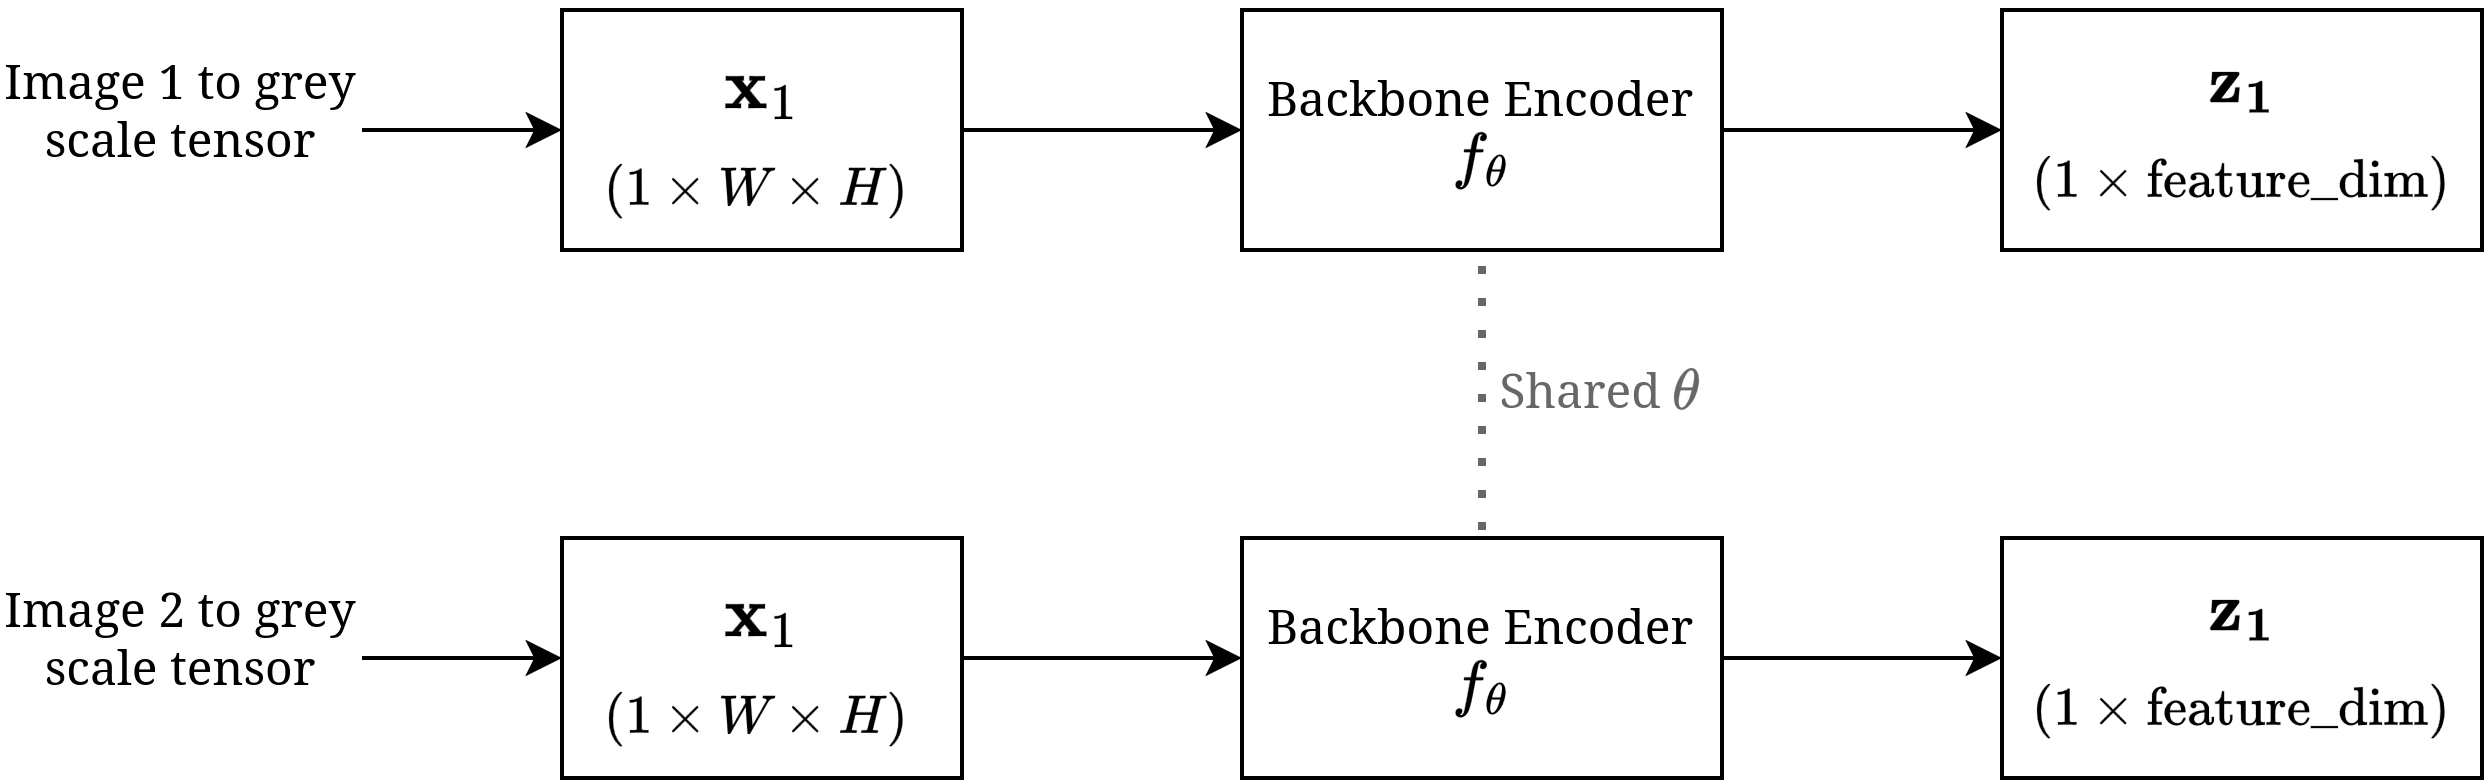
\includegraphics[width=0.8\textwidth]{images/siamese-architecture.drawio.png}
    \caption{Overview of the encoder architecture up to the feature dimension.}
    \label{fig:encoder-architecture}
\end{figure}
% 


Our framework implements a modular Siamese architecture composed of three main components: the backbone encoder, the projection head, and the decision mechanism. All components utilize shared weights between the twin networks to ensure symmetric feature extraction.

\subsubsection{Backbone Encoder}

The backbone encoder extracts high-level discriminative features from input handwriting images. We systematically evaluate six state-of-the-art convolutional neural network architectures organized into three architectural families:

\begin{itemize}
\item \textbf{ResNet family:} ResNet18 and ResNet34 with residual connections for deep feature learning
\item \textbf{EfficientNet family:} EfficientNet-B0 and EfficientNet-B1 employing compound scaling strategies
\item \textbf{MobileNet family:} MobileNetV3-Small and MobileNetV3-Large utilizing depthwise separable convolutions for efficiency
\end{itemize}

All backbones are initialized with ImageNet pre-trained weights to leverage transfer learning from large-scale visual recognition tasks. To adapt RGB-pretrained models to grayscale handwriting inputs while preserving the learned representations, the first convolutional layer is not reinitialized. Instead, the pretrained convolutional filters corresponding to the three RGB input channels are aggregated into a single-channel representation.

Specifically, given the original first convolutional layer:

\begin{equation}
\text{Conv2d}(3, C_{\text{out}}, \text{kernel\_size}, \text{stride}, \text{padding}, \text{bias}=\text{False}),
\end{equation}

the weights of the three input channels are averaged to produce a single-channel kernel:

\begin{equation}
W_{\text{gray}} = \frac{1}{3} \sum_{c=1}^{3} W_c,
\end{equation}

where $W_c$ denotes the pretrained weights associated with the $c$-th RGB channel.  
The resulting weights are then used to define a grayscale-compatible convolutional layer:

\begin{equation}
\text{Conv2d}(1, C_{\text{out}}, \text{kernel\_size}, \text{stride}, \text{padding}, \text{bias}=\text{False}),
\end{equation}

thereby retaining the pretrained knowledge of the original model while enabling processing of single-channel input images.

\subsubsection{Head Networks}

Depending on the training objective, different head architectures are employed on top of the shared backbone encoder.

\paragraph{Similarity (Decision) Head for BCE Models}

For BCE-based Siamese models, verification is formulated as a binary classification problem. Given two input images, the encoder produces two feature embeddings:

\begin{equation}
\mathbf{z}_1,\mathbf{z}_2 \in \mathbb{R}^{D}
\end{equation}

where $D$ denotes the embedding dimensionality. The two embeddings are concatenated to form the input representation of the decision head:

\begin{equation}
\mathbf{h}^{(0)}
=
[\mathbf{z}_1;\mathbf{z}_2]
\in
\mathbb{R}^{2D}
\end{equation}

The decision head is implemented as a fully connected network with progressively reduced dimensionality:

\begin{equation}
\mathbb{R}^{2D}
\rightarrow
\mathbb{R}^{32}
\rightarrow
\mathbb{R}^{16}
\rightarrow
\mathbb{R}^{8}
\rightarrow
\mathbb{R}^{4}
\rightarrow
\mathbb{R}^{2}
\rightarrow
[0,1]
\end{equation}

Each hidden layer applies a linear transformation followed by batch normalization\cite{ioffe2015batchnorm}, ReLU activation, and dropout regularization. The generic transformation is defined as:

\begin{equation}
\mathbf{h}^{(l+1)}
=
\mathrm{Dropout}_{p_l}
\left(
\mathrm{ReLU}
\left(
\mathrm{BN}
\left(
\mathbf{W}^{(l)}\mathbf{h}^{(l)}
+
\mathbf{b}^{(l)}
\right)
\right)
\right)
\end{equation}

where:

\begin{equation}
\mathbf{W}^{(l)}
\in
\mathbb{R}^{d_{l+1}\times d_l},
\qquad
\mathbf{b}^{(l)}
\in
\mathbb{R}^{d_{l+1}}
\end{equation}

and $d_l$ and $d_{l+1}$ denote the input and output dimensionalities of the $l$-th fully connected layer.

The dropout probabilities applied after each hidden layer are:

\begin{equation}
p_l \in \{0.20,0.20,0.18,0.16,0.12\}
\end{equation}

After the final hidden representation:

\begin{equation}
\mathbf{h}^{(5)}\in\mathbb{R}^{2}
\end{equation}

the last linear layer produces a scalar logit:
\begin{equation}
a
=
\mathbf{W}^{(5)}\mathbf{h}^{(5)}
+
b^{(5)}
\end{equation}
where:
\begin{equation}
\mathbf{W}^{(5)}\in\mathbb{R}^{1\times2},
\qquad
b^{(5)}\in\mathbb{R}
\end{equation}

The final similarity score is obtained through a sigmoid activation:

\begin{equation}
\hat{y}
=
\sigma(a)
=
\frac{1}{1+e^{-a}}
\end{equation}

where:

\begin{equation}
\hat{y}\in(0,1)
\end{equation}

represents the predicted probability that the two input images belong to the same writer.

Unlike metric-learning approaches, this BCE-based decision head does not explicitly
enforce geometric constraints on the embedding space. Instead, it learns a discriminative
similarity function directly from the concatenated encoder representations, as illustrated
in Figure~\ref{fig:bce-architecture}.

\begin{figure}[h!]
    \centering
    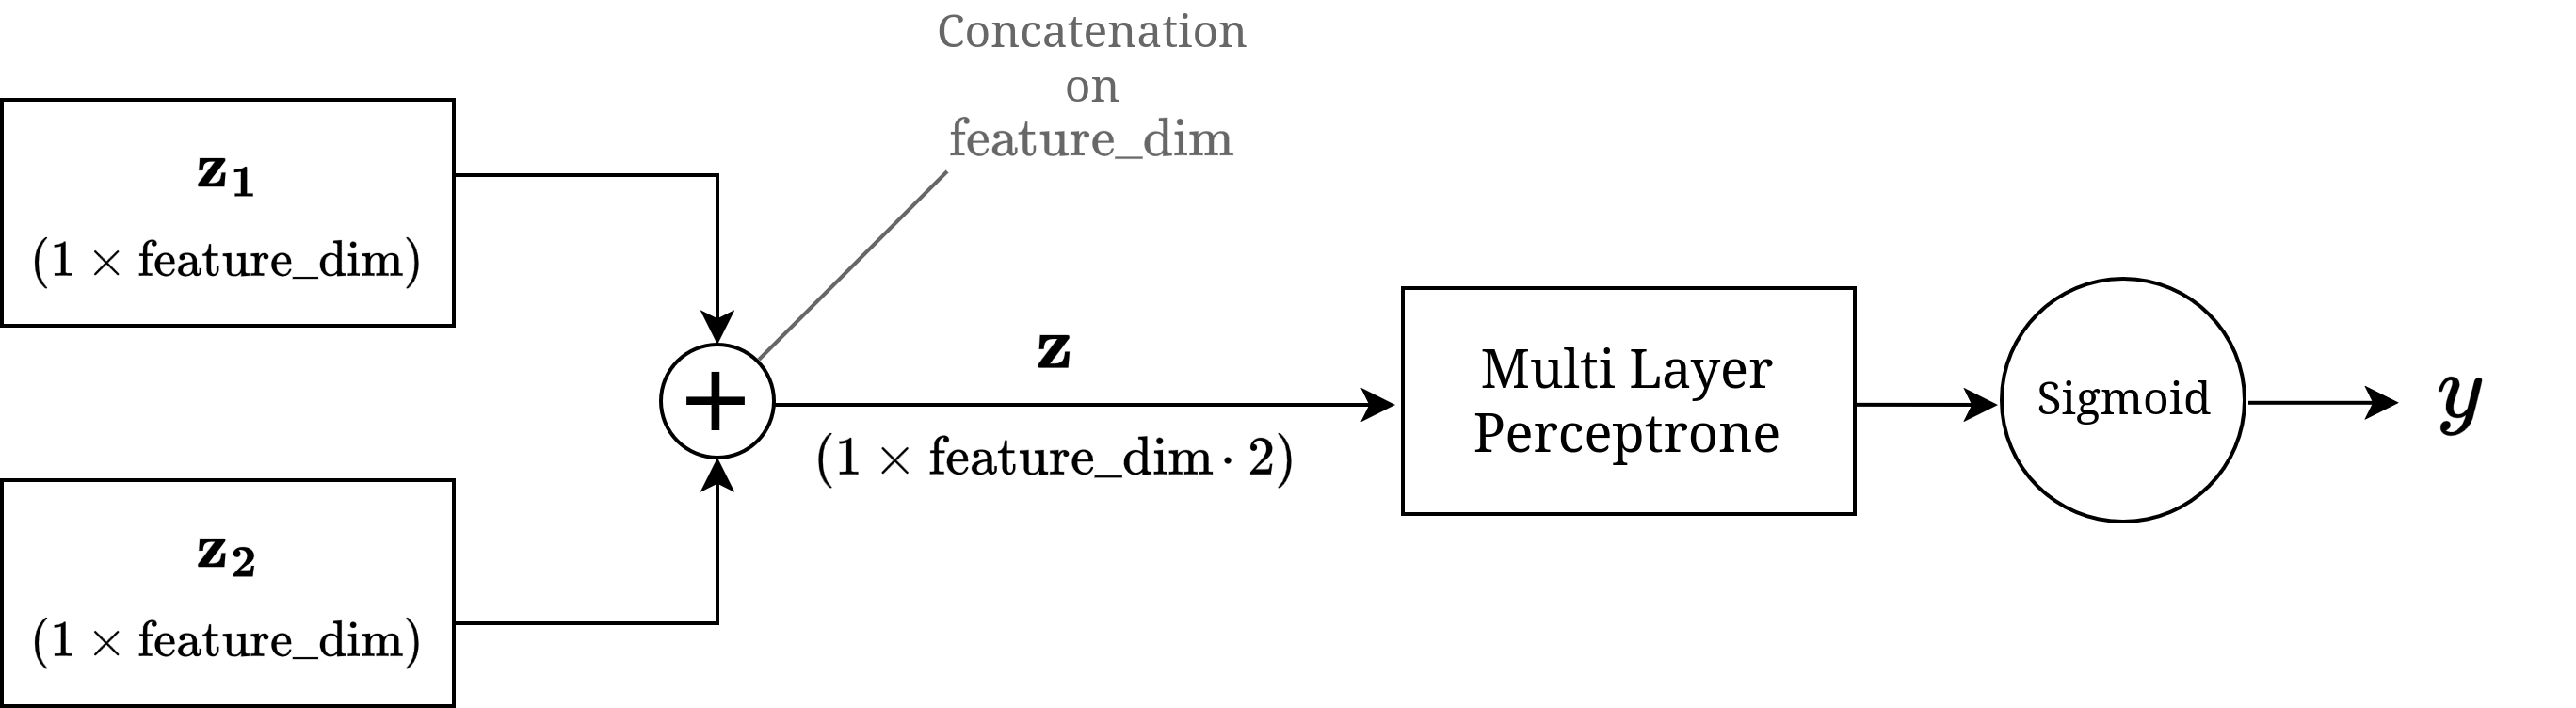
\includegraphics[width=1.0\textwidth]{images/bce-architecture.drawio.png}
    \caption{Similarity (decision) head for BCE-based models. The concatenated
    embeddings $\mathbf{z}_1$ and $\mathbf{z}_2$ are processed by a multi-layer
    perceptron followed by a sigmoid activation, producing a similarity score
    $\hat{y} \in (0,1)$.}
    \label{fig:bce-architecture}
\end{figure}

\paragraph{Projection Head for Contrastive and Triplet Models}

For contrastive and triplet learning objectives, the shared encoder extracts feature representations from two input images:

\begin{equation}
\mathbf{z}_1,\mathbf{z}_2\in\mathbb{R}^{D}
\end{equation}

where $D$ denotes the dimensionality of the backbone features. The two feature vectors are independently processed by the same projection head with shared parameters:

\begin{equation}
\mathbf{e}_1=g_{\phi}(\mathbf{z}_1),
\qquad
\mathbf{e}_2=g_{\phi}(\mathbf{z}_2)
\end{equation}

where $g_{\phi}$ denotes the MLP projection head and $\phi$ represents its learnable
parameters, as depicted in Figure~\ref{fig:contrastive-architecture}.

\begin{figure}[h!]
    \centering
    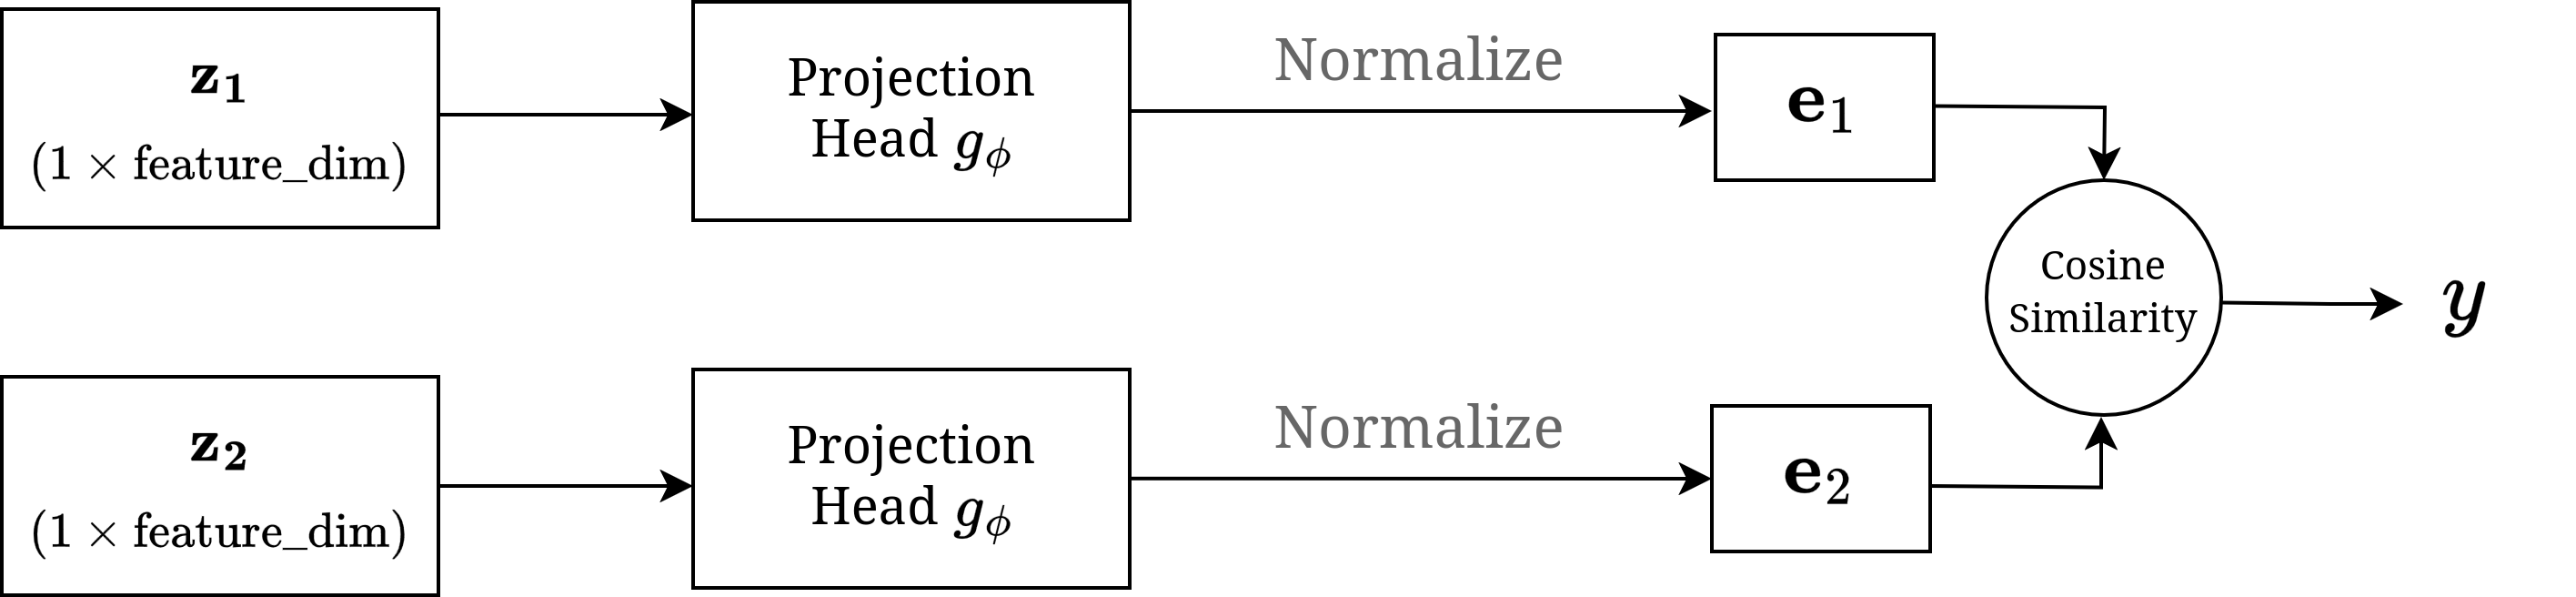
\includegraphics[width=1.0\textwidth]{images/contrastive-architecture.drawio.png}
    \caption{Projection head for contrastive and triplet learning models. Backbone
    features $\mathbf{z}_1$ and $\mathbf{z}_2$ are independently mapped by the shared
    projection head $g_\phi$, $\ell_2$-normalized, and compared via cosine similarity.}
    \label{fig:contrastive-architecture}
\end{figure}

The projection network maps the backbone features into a lower-dimensional embedding space according to:

\begin{equation}
\mathbb{R}^{D}
\rightarrow
\mathbb{R}^{1024}
\rightarrow
\mathbb{R}^{512}
\rightarrow
\mathbb{R}^{256}
\rightarrow
\mathbb{R}^{32}
\end{equation}

Each hidden layer applies a linear transformation followed by batch normalization, 
ReLU activation, and dropout regularization:

\begin{equation}
\mathbf{h}^{(l+1)}
=
\mathrm{Dropout}_{p_l}
\left(
\mathrm{ReLU}
\left(
\mathrm{BN}
\left(
\mathbf{W}^{(l)}
\mathbf{h}^{(l)}
+
\mathbf{b}^{(l)}
\right)
\right)
\right)
\end{equation}

where:

\begin{equation}
\mathbf{W}^{(l)}
\in
\mathbb{R}^{d_{l+1}\times d_l},
\qquad
\mathbf{b}^{(l)}
\in
\mathbb{R}^{d_{l+1}}
\end{equation}

The final projection layer produces the 32-dimensional embedding without applying any non-linear activation:

\begin{equation}
\mathbf{e}_i
=
\mathbf{W}^{(3)}
\mathbf{h}^{(3)}_i
+
\mathbf{b}^{(3)},
\qquad i\in\{1,2\}
\end{equation}

The resulting embeddings are normalized independently using $\ell_2$ normalization:

\begin{equation}
\hat{\mathbf{e}}_i
=
\frac{\mathbf{e}_i}
{\|\mathbf{e}_i\|_2},
\qquad i\in\{1,2\}
\end{equation}

obtaining unit-length embeddings:

\begin{equation}
\hat{\mathbf{e}}_1,\hat{\mathbf{e}}_2\in\mathbb{R}^{32},
\qquad
\|\hat{\mathbf{e}}_1\|_2=\|\hat{\mathbf{e}}_2\|_2=1
\end{equation}

The dropout probabilities applied after the hidden layers are:

\begin{equation}
p_l\in\{0.20,0.20,0.16\}
\end{equation}

The two normalized embeddings are then compared through cosine similarity:

\begin{equation}
s_{12}
=
\frac{\hat{\mathbf{e}}_1^T\hat{\mathbf{e}}_2}
{\|\hat{\mathbf{e}}_1\|_2\|\hat{\mathbf{e}}_2\|_2}
\end{equation}

Since the embeddings are normalized:

\begin{equation}
s_{12}=\hat{\mathbf{e}}_1^T\hat{\mathbf{e}}_2
\end{equation}

For contrastive learning, the similarity score is optimized directly by minimizing the distance between genuine pairs and enforcing a margin separation between impostor pairs.

For triplet learning, the same shared embedding function is applied to additional samples during training. The resulting embeddings are compared through relative similarities, enforcing that the anchor-positive similarity is larger than the anchor-negative similarity by a margin:

\begin{equation}
s_{ap}>s_{an}+m
\end{equation}

Therefore, both approaches use the same shared projection architecture and produce normalized embeddings suitable for metric comparison. The difference lies only in the optimization objective: contrastive learning operates on pairs of embeddings, whereas triplet learning optimizes relative relationships among anchor, positive, and negative samples.

\subsection{Loss Functions}

We investigate three loss formulations representing different approaches to the verification problem:

\subsubsection{Binary Cross-Entropy Loss}

BCE treats verification as direct similarity classification:
\begin{equation}
\mathcal{L}_{\text{BCE}} = -\frac{1}{N}\sum_{i=1}^{N} \left[y_i \log(\hat{y}_i) + (1-y_i)\log(1-\hat{y}_i)\right]
\end{equation}

where $\hat{y}_i \in [0,1]$ is the predicted similarity score and $y_i \in \{0,1\}$ is the ground truth label. This formulation provides stable gradients and reliable convergence but does not explicitly structure the embedding space according to metric properties.

\subsubsection{Contrastive Loss}

Contrastive Loss explicitly optimizes pairwise distances with margin-based separation:
\begin{equation}
\mathcal{L}_{\text{Contrastive}} =
\frac{1}{N}\sum_{i=1}^{N}
\left[
y_i d_i^2 +
(1-y_i)\max(m-d_i,0)^2
\right]
\end{equation}

where $d_i = 1-s_i$ represents the cosine-based distance derived from the cosine similarity $s_i$, and $m$ is the margin hyperparameter. The cosine similarity is computed between L2-normalized feature embeddings, resulting in $s_i \in [-1,1]$ and $d_i \in [0,2]$. Genuine pairs ($y_i=1$) minimize the distance between embeddings, while impostor pairs ($y_i=0$) are penalized when their distance falls below the margin threshold $m$, encouraging separation in the embedding space. We set $m=1.0$ based on preliminary experiments.

\subsubsection{Triplet Loss}

Triplet Loss enforces relative distance constraints by optimizing the separation between anchor-positive and anchor-negative pairs. Given a triplet composed of an anchor sample, a positive sample from the same writer, and a negative sample from a different writer, the loss is defined as:

\begin{equation}
\mathcal{L}_{\text{Triplet}} =
\frac{1}{N}\sum_{i=1}^{N}
\max\left(d_{ap}^{(i)} - d_{an}^{(i)} + m, 0\right)
\end{equation}

where $d_{ap}$ and $d_{an}$ denote the cosine distances between the anchor-positive and anchor-negative embeddings, respectively. The cosine distance is defined as:

\begin{equation}
d(x,y)=1-\cos(x,y)
\end{equation}

where cosine similarity is computed between L2-normalized embeddings, resulting in $d(x,y) \in [0,2]$. The loss encourages the distance between samples from the same writer to be smaller than the distance between samples from different writers by at least a margin $m$. When the constraint

\begin{equation}
d_{ap} + m < d_{an}
\end{equation}

is satisfied, the contribution to the loss becomes zero, meaning that the triplet already satisfies the desired separation. We set $m=0.5$ based on preliminary experiments, providing a balance between intra-class compactness and inter-class separation.

\subsection{Training Strategies}

\subsubsection{Dynamic Negative Sampling}

Class imbalance poses a significant challenge in writer verification \cite{he2009imbalanced}.
Given $W$ writers with $N_w$ samples each, the number of genuine pairs scales as
$O(W \cdot N_w^2)$ while impostor pairs scale as $O(W^2 \cdot N_w^2)$, creating severe
imbalance with impostor pairs vastly outnumbering genuine pairs.

We address this through epoch-wise dynamic negative resampling, a random undersampling
strategy applied to the majority class \cite{he2009imbalanced}. All genuine pairs are
preserved (being the minority class), while impostor pairs are randomly resampled each
epoch to maintain a target positive ratio. This strategy exposes the model to diverse
negative examples across epochs while maintaining balanced training signals:

\begin{algorithm}[H]
\caption{Dynamic Negative Sampling Strategy}
\begin{algorithmic}[1]
\State Generate all genuine pairs $\mathcal{P}_{\text{genuine}}$ from same-writer samples
\State Generate complete pool of impostor pairs $\mathcal{P}_{\text{impostor}}$
\State Compute required impostor count: $N_{\text{imp}} = \lfloor N_{\text{gen}} \cdot (1-r)/r \rfloor$
\For{epoch $e = 1$ to $E$}
    \State Sample $\mathcal{P}_{\text{impostor}}^{(e)} \subset \mathcal{P}_{\text{impostor}}$ with $|\mathcal{P}_{\text{impostor}}^{(e)}| = N_{\text{imp}}$
    \State $\mathcal{D}^{(e)} = \mathcal{P}_{\text{genuine}} \cup \mathcal{P}_{\text{impostor}}^{(e)}$
    \State Shuffle $\mathcal{D}^{(e)}$
    \State Train on $\mathcal{D}^{(e)}$
\EndFor
\end{algorithmic}
\end{algorithm}

where $r$ is the target positive ratio (set to 0.5 for balanced training).

\subsubsection{Selective Layer Freezing}

To prevent overfitting on limited handwriting data while maintaining transfer learning benefits, 
we implement selective layer freezing in the backbone encoder. The first $L_f$ convolutional 
layers remain frozen with gradients disabled, preserving generic low-level features learned from ImageNet, 
while deeper layers undergo fine-tuning for task-specific adaptation:

\begin{equation}
\theta = \{\theta_{\text{frozen}}, \theta_{\text{trainable}}\}, \quad \text{where} \quad \frac{\partial \mathcal{L}}{\partial \theta_{\text{frozen}}} = 0
\end{equation}

We freeze $L_f = 3$ initial layers for all backbone architectures trained, striking a balance between preserving pretrained knowledge and allowing 
domain adaptation.

\subsubsection{Regularization Techniques}

To prevent overfitting, we employ a comprehensive regularization strategy:

\begin{itemize}
\item \textbf{Graduated Dropout:} Starting from a base rate of $0.2$, dropout is scaled by a per-layer factor (1.0, 1.0, 0.9, 0.8, 0.6) so that deeper layers retain more expressiveness. This yields rates of $\{0.20,0.20,0.18,0.16,0.12\}$ for the five-layer BCE decision head and $\{0.20,0.20,0.16\}$ for the three-layer contrastive/triplet projection head.
\item \textbf{Weight Decay:} Decoupled weight decay (as implemented by AdamW) with coefficient $\lambda = 10^{-4}$ applied to all trainable parameters prevents weight magnitude explosion.
\item \textbf{Batch Normalization:} Applied after each linear transformation to stabilize training dynamics and provide implicit regularization through mini-batch statistics.

\item \textbf{Data Augmentation:} Training images undergo random transformations including rotation ($\pm15°$) and random resized crops (90-110\% of original size) to simulate natural writing variations while preserving character structure.
\end{itemize}

\subsection{Optimization}

We employ the AdamW\cite{loshchilov2019adamw} optimizer with hyperparameters adapted to model capacity:

\begin{equation}
\text{lr} = \begin{cases}
5 \times 10^{-5} & \text{if } |\theta| > 15 \times 10^6 \\
1 \times 10^{-4} & \text{otherwise}
\end{cases}
\end{equation}

where $|\theta|$ denotes the total number of trainable parameters. Additional optimizer parameters are set to $\beta_1 = 0.9$, $\beta_2 = 0.999$, $\epsilon = 10^{-8}$, and weight decay $\lambda = 10^{-4}$.

Learning rate scheduling employs ReduceLROnPlateau with factor 0.5 and patience 2 epochs, monitoring validation loss for dynamic adaptation. Early stopping with patience 5 epochs prevents overfitting while allowing sufficient convergence time, terminating training when validation loss fails to improve for the patience period.
%============================================================
% SEZIONE: Experimental Setup
%============================================================
\section{Experimental Setup}\label{sec:experiments}

\subsection{Datasets}

We evaluate our framework on two standard handwriting verification datasets. Due to the modular design, the framework supports any dataset organized with writer subdirectories containing handwriting samples. For this study, we use datasets with varying numbers of writers and samples per writer to assess generalization across different data scales.

Images are preprocessed to grayscale and resized to 448×448 pixels, balancing computational efficiency with fine detail preservation. This resolution is sufficient to capture stroke characteristics while remaining manageable for modern GPUs.

\subsection{Data Preprocessing}

All datasets undergo a rigorous preprocessing pipeline to normalize images while preserving handwriting characteristics. 
The pipeline combines Otsu's binarization, morphological operations, and adaptive cropping strategies 
tailored to each dataset's structure. Binarization is used exclusively as an auxiliary guide to \emph{compute} 
crop coordinates and content masks; the pixel values that are ultimately cropped, resized, and saved to disk 
always come from the original \emph{grayscale} image, never from the binary mask itself.

In brief: each grayscale image is Otsu-thresholded to obtain a binary mask, which is used to (i) detect IAM guide 
lines, (ii) locate left-margin and top/bottom black regions, and (iii) compute tight-crop bounding boxes 
via axial projections. These coordinates are then applied to the grayscale image, which is cropped, centered on 
a square canvas, and resized to 448×448 with area interpolation. IAM full-form images additionally undergo guide-line 
detection and removal via morphological opening, with the handwritten region extracted according to the number of 
detected lines (falling back to a fixed region when detection is unreliable). RIMES text lines are instead 
height-normalized per writer and vertically stacked into groups of 5 to form 448×448 batches.

The full mathematical formulation of these steps (Otsu thresholding, projection-based tight cropping, IAM guide-line 
detection rules, RIMES height normalization and batching, visual examples, and associated fallback/safeguard conditions) 
is provided in Appendix~\ref{app:preprocessing}, together with the exact parameter values used ($\rho = 0.018$ for 
RIMES, $\rho = 0.02$ for IAM, padding, trim, and batching constants). All these seemingly arbitrary configuration 
choices are carefully designed with the final dataset in mind, in particular to avoid issues with the models or 
loss functions such as having too few positive/negative pairs or too few triplets, which could make training more 
difficult.

\subsection{Dataset Statistics Analysis}
\label{subsec:dataset-stats}

After preprocessing, we analyze the distribution of images per author across the two resulting datasets, as this directly informs downstream design choices such as batching strategy and writer-level splitting. Table~\ref{tab:dataset-stats} summarizes the key statistics computed on the preprocessed IAM and RIMES datasets.

\begin{table}[h]
\centering
\caption{Summary statistics of images per author for the preprocessed IAM and RIMES datasets.}
\label{tab:dataset-stats}
\begin{tabular}{lrrrrrr}
\toprule
\textbf{Dataset} & \textbf{Authors} & \textbf{Tot. Images} & \textbf{Mean/Author} & \textbf{Median/Author} & \textbf{Std/Author} & \textbf{Min/Max} \\
\midrule
IAM   & 657  & 1539 & 2.34 & 1.0 & 3.03 & 1 / 59 \\
RIMES & 1500 & 5046 & 3.36 & 3.0 & 1.27 & 1 / 10 \\
\bottomrule
\end{tabular}
\end{table}

IAM comprises 657 authors contributing a total of 1539 processed images, with a mean of 2.34 images per author but a median of only 1.0, indicating a strongly right-skewed distribution; this is confirmed by the high standard deviation (3.03) relative to the mean, and by the presence of an extreme outlier author with 59 images, more than an order of magnitude above the median. RIMES, in contrast, comprises 1500 authors and 5046 total processed images (batches), with mean and median again fairly close (3.36 and 3.0 respectively) and a moderate standard deviation (1.27), with a maximum of 10 images per author. The corresponding per-author histograms and boxplot comparison, which visually confirm this asymmetry (IAM dominated by a large spike at 1--2 images per author with a long sparse tail, RIMES broader and more centrally distributed), are reported in Appendix~\ref{app:dataset-stats-figures}.

This asymmetry has practical implications for the training pipeline: since IAM images already correspond to full, variable-length handwritten samples (one 448×448 image per crop), no further batching is applied, and the heavy-tailed per-author distribution is instead handled through a writer-level (rather than image-level) train/validation/test split, preventing data leakage across sets. For RIMES, the "images" counted here correspond to the stacked 448×448 batches produced by the line-grouping procedure (Appendix~\ref{app:preprocessing}); the broader spread around 3 batches per author, compared to IAM, reflects the larger and more variable number of lines each RIMES writer contributed, combined with the fixed batch size $N_{\text{batch}}=5$.

\subsection{Experimental Protocol}

\subsubsection{Train/Validation/Test Splitting and Dataset Pairings}
\label{subsubsec:dataset-pairings}

Each candidate backbone/loss configuration is evaluated on four
train$\to$evaluation dataset pairings (IAM$\to$IAM, IAM$\to$RIMES,
RIMES$\to$IAM, RIMES$\to$RIMES), for $6(backbones)\times3(losses)\times4(pairings)=72$ trained
models in total.

For the two \textbf{within-dataset} pairings (IAM$\to$IAM,
RIMES$\to$RIMES), the source dataset is writer-disjointly split into
three subsets: 70\% training, 10\% validation (\texttt{val\_size}
$=0.1$, used for model selection / early-stopping monitoring), and
20\% test (\texttt{test\_size} $=0.2$, held out and used only for the
final comprehensive evaluation), with a fixed random seed of 42.

For the two \textbf{cross-dataset} pairings (IAM$\to$RIMES,
RIMES$\to$IAM), the model is trained on the \emph{entire} source
dataset (all of its writers), while the target dataset is itself split
writer-disjointly into a 10\% validation subset (monitoring/early
stopping) and a 90\% test subset, the latter used for the final
evaluation reported throughout this paper. This setting assesses the
ability of a model trained on one handwriting dataset to generalize to
a different handwriting domain and data-collection protocol.

Exact writer and pair counts per split are given in
Table~\ref{tab:protocol} (Section~\ref{sec:protocol}); these counts are
confirmed identical across all backbone/loss combinations within a
given split, since the writer-level split depends only on the fixed
random seed and dataset identity, not on backbone or loss.

For all training configurations, negative samples are resampled every epoch, since the number of possible negative pairs is substantially larger than the number of positive pairs. Resampling therefore allows the model to observe a wider variety of negative examples throughout training, rather than repeatedly using the same subset of negative pairs.

This choice is also motivated by the intended real-world application: in forensic handwriting and signature examination, cases are not submitted to an examiner at random, but precisely because the authenticity of a signature or document is already in question---an instance of what is known in the forensic statistics literature as an \emph{ascertainment} (or \emph{selection}) bias effect on casework composition \cite{rosenblum2024incorrect}\footnote{The cited work discusses this effect in the context of firearms examiner casework; we adopt it here as a conceptually analogous argument, as no equivalent study (at the best of our knowledge) specifically quantifying casework composition exists for forensic handwriting/signature examination.}. As a result, the population of samples an examiner actually evaluates is skewed toward disputed, and often forged, material relative to the general population of signatures. Exposing the model to a wide and varied set of negative examples during training is therefore consistent with this real-world prior: a system intended to support forgery detection should be robust across a broad range of negative (forged) cases, rather than a narrow, fixed subset.

No resampling is applied to the validation or test sets, which remain fixed throughout each experiment. Each model is trained from scratch for every architecture/loss/dataset-pairing combination, with early stopping monitored using the corresponding validation set.

\subsubsection{Hyperparameters}

All 72 configurations of the main sweep share a single uniform
hyperparameter configuration: batch size 16, 3 frozen backbone encoder
layers, dropout 0.2, and margins 0.5 (Contrastive) / 0.3 (Triplet), matching
the values introduced in Section~\ref{sec:methodology}.
A complete list of representative hyperparameters, including values not
otherwise discussed in the main text (maximum epochs, embedding
dimension, data-loading workers, etc), is given in
Appendix~\ref{app:hyperparams}.
\section{Results}
\label{sec:results}

\subsection{Evaluation protocol} \label{sec:protocol}

We evaluate six backbones (EfficientNet-B0/B1, MobileNetV3-Small/Large, ResNet-18/34) trained under three losses (BCE, Contrastive, Triplet) on four train$\to$test dataset pairings (Section~\ref{subsubsec:dataset-pairings}), resulting in 72 trained configurations in total.

For all configurations, pair generation follows the same procedure. Genuine pairs are generated once and kept fixed throughout training, while impostor pairs are drawn from a larger candidate pool and resampled every epoch. The target positive ratio is set to 50\%, so that the number of impostor pairs sampled at each epoch equals the number of available genuine pairs. This produces balanced epoch datasets while allowing the model to observe different negative pairs across epochs. The same pair-generation and resampling strategy is used independently of the backbone, loss function, or dataset split.

\begin{table}[htbp]
\centering
\caption{Evaluation protocol and pair counts for each dataset split. Writer counts refer to the train, validation, and test partitions. For each partition, the number of genuine and impostor pairs is equal, corresponding to the 50\% positive-ratio setting. Genuine pairs are fixed, whereas impostor pairs are sampled from a larger candidate pool and resampled every epoch. The same pair-generation procedure is used across all backbone/loss configurations, so pair counts are identical across the 18 configurations within each split.}
\label{tab:protocol}
\begin{tabular}{lrrrccc}
\toprule
Split & Train w. & Val w. & Test w. &
Gen/Imp (train) &
Gen/Imp (val) &
Gen/Imp (test) \\
\midrule
IAM $\to$ IAM
& 459 & 66 & 132
& 3{,}262 / 3{,}262
& 310 / 310
& 479 / 479 \\

IAM $\to$ RIMES
& 657 & 150 & 1{,}350
& 4{,}051 / 4{,}051
& 746 / 746
& 6{,}429 / 6{,}429 \\

RIMES $\to$ IAM
& 1{,}500 & 65 & 592
& 7{,}175 / 7{,}175
& 207 / 207
& 3{,}844 / 3{,}844 \\

RIMES $\to$ RIMES
& 1{,}049 & 150 & 301
& 5{,}023 / 5{,}023
& 625 / 625
& 1{,}527 / 1{,}527 \\
\bottomrule
\end{tabular}
\end{table}

For the IAM$\to$IAM split, the pair-generation procedure produces 3,262 fixed genuine training pairs and 310 fixed genuine validation pairs. The corresponding impostor candidate pools contain 589,154 and 12,251 possible pairs, respectively. At each epoch, 3,262 impostors are sampled for training and 310 for validation, yielding 6,524 and 620 pairs per epoch, respectively, with an actual positive ratio of 50\%. On the test set, 479 genuine and 479 impostor pairs are evaluated, resulting in 958 evaluation pairs. The same generation and resampling procedure is applied to the other three dataset splits; therefore, the pair counts reported in Table~\ref{tab:protocol} are shared by all 18 backbone/loss configurations within each split.

IAM$\to$IAM is the smallest-identity split (132 test writers, 958 evaluation pairs) and therefore likely carries the widest evaluation uncertainty among the same-dataset splits below; RIMES contributes $\sim2.3\times$ more writers than IAM overall (1{,}500 vs.\ 657), a plausible contributing factor to the asymmetry between the two cross-dataset performances (Section~\ref{sec:cross-dataset}).

Metrics follow the classical FAR/FRR convention. Classification metrics (accuracy/precision/recall/F1) are computed at the EER threshold, not an independently calibrated one.

As only a single seed is trained per configuration, all figures below are point estimates from a single trained model per (backbone, loss, split); no per-model bootstrap confidence intervals were available for this revision (Section~\ref{sec:limitations}). Mean $\pm$ std figures in Tables~\ref{tab:same-dataset}--\ref{tab:cross-dataset} are across-backbone summary statistics (Table~5), not evaluation-set confidence intervals.


\subsection{Same-dataset performance}
\label{sec:same-dataset}

\begin{table}[htbp]
  \centering
  \caption{Same-dataset verification performance (mean $\pm$ std across
  6 backbones; Table~5).}
  \label{tab:same-dataset}
  \small
  \begin{tabular}{llccc}
    \toprule
    Loss & Split & AUC & EER (\%) & $d'$ \\
    \midrule
    BCE         & IAM$\to$IAM     & 0.956 $\pm$ 0.025 & 9.0 $\pm$ 4.0  & 3.10 \\
    Contrastive & IAM$\to$IAM     & \textbf{0.990} $\pm$ 0.004 & \textbf{4.9} $\pm$ 1.3 & \textbf{3.64} \\
    Triplet     & IAM$\to$IAM     & 0.924 $\pm$ 0.029 & 15.3 $\pm$ 3.6 & 1.84 \\
    \midrule
    BCE         & RIMES$\to$RIMES & 0.734 $\pm$ 0.180 & 30.9 $\pm$ 15.3 & 1.03 \\
    Contrastive & RIMES$\to$RIMES & \textbf{0.927} $\pm$ 0.007 & \textbf{12.9} $\pm$ 1.1 & \textbf{2.12} \\
    Triplet     & RIMES$\to$RIMES & 0.888 $\pm$ 0.014 & 18.3 $\pm$ 1.1 & 1.69 \\
    \bottomrule
  \end{tabular}
\end{table}

Contrastive is the best-performing loss by a wide margin on both
same-dataset splits, and has the smallest across-backbone variance of
the three losses. BCE shows by far the largest across-backbone spread
on RIMES$\to$RIMES ($\sigma_{\text{AUC}}=0.180$ vs.\ $0.007$ for
Contrastive), directly attributable to the collapsed-model instability
documented in Section~\ref{sec:per-backbone}. The single best
configuration per split (Table~4) is MobileNetV3-Large + Contrastive
on IAM$\to$IAM (AUC $=0.995$, EER $=3.1\%$), and ResNet-18 +
Contrastive on RIMES$\to$RIMES (AUC $=0.934$, EER $=11.5\%$):
Contrastive wins both at the aggregate and the best-single-model
level.

\subsection{Cross-dataset generalization}
\label{sec:cross-dataset}

\begin{table}[htbp]
  \centering
  \caption{Cross-dataset verification performance (mean $\pm$ std
  across 6 backbones; Table~5).}
  \label{tab:cross-dataset}
  \small
  \begin{tabular}{llccc}
    \toprule
    Loss & Split & AUC & EER (\%) & $d'$ \\
    \midrule
    BCE         & IAM$\to$RIMES   & 0.621 $\pm$ 0.082 & 40.2 $\pm$ 6.9  & 0.50 \\
    Contrastive & IAM$\to$RIMES   & \textbf{0.738} $\pm$ 0.032 & \textbf{32.2} $\pm$ 2.4 & 0.77 \\
    Triplet     & IAM$\to$RIMES   & 0.699 $\pm$ 0.034 & 35.5 $\pm$ 2.5 & 0.64 \\
    \midrule
    BCE         & RIMES$\to$IAM   & 0.715 $\pm$ 0.133 & 32.9 $\pm$ 12.8 & 0.90 \\
    Contrastive & RIMES$\to$IAM   & \textbf{0.950} $\pm$ 0.014 & \textbf{11.7} $\pm$ 2.3 & 2.13 \\
    Triplet     & RIMES$\to$IAM   & 0.869 $\pm$ 0.048 & 20.4 $\pm$ 4.9 & 1.31 \\
    \bottomrule
  \end{tabular}
\end{table}

Contrastive again dominates both cross-dataset splits. RIMES$\to$IAM
(training on the larger, 1{,}500-writer pool) clearly outperforms
IAM$\to$RIMES under every loss -- for Contrastive, AUC $0.950$ vs.\
$0.738$ -- consistent with source writer-pool size
(Table~\ref{tab:protocol}) as a contributing factor. Best individual
configurations (Table~4): EfficientNet-B1 + Contrastive on
IAM$\to$RIMES (AUC $=0.772$, EER $=29.6\%$), EfficientNet-B0 +
Contrastive on RIMES$\to$IAM (AUC $=0.967$, EER $=8.2\%$).

Figure~\ref{fig:same-vs-cross} summarizes the same-vs-cross
generalization gap aggregated across all 6 backbones: BCE shows the
largest AUC drop, Contrastive an intermediate one, and Triplet the
smallest but also the lowest absolute same-dataset AUC among the
three losses.

\begin{figure}[htbp]
  \centering
  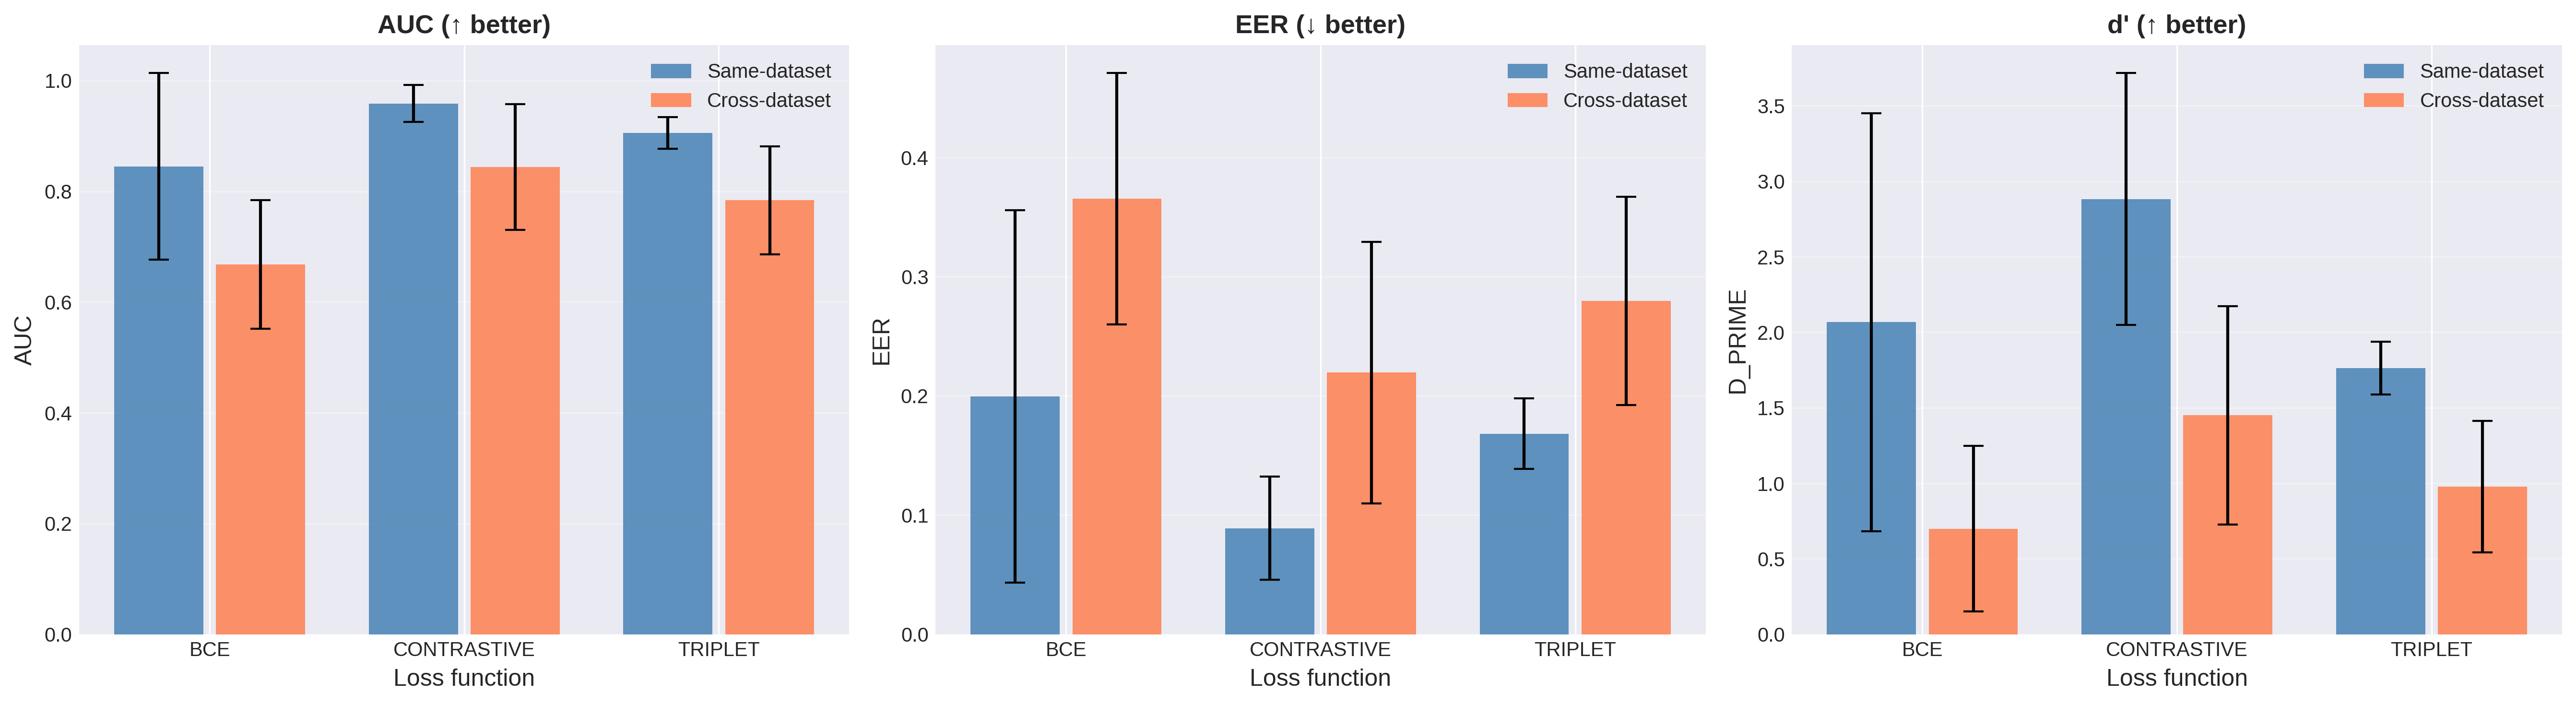
\includegraphics[width=\textwidth]{images/same_vs_cross_comparison_aggregated.png}
  \caption{AUC, EER and $d'$, same-dataset vs.\ cross-dataset,
  aggregated per loss (mean $\pm$ std across 6 backbones).}
  \label{fig:same-vs-cross}
\end{figure}

\subsection{Fixed operating points (FAR/FRR trade-off)}
\label{sec:operating-points}

Fixed operating points provide a complementary view of verification performance by quantifying the proportion of genuine pairs correctly accepted (GAR) under stringent false-acceptance constraints. In particular, FAR values of 1\% and 0.1\% represent increasingly conservative operating conditions, making the corresponding GAR values informative of how well a model maintains genuine-user acceptance while limiting false matches. The results also highlight the substantial impact of the dataset shift: while the best same-dataset configuration maintains relatively high GAR at both operating points, cross-dataset performance deteriorates markedly, especially at FAR$=0.1\%$. This indicates that a high overall discrimination capability does not necessarily translate into robust performance in low-FAR operating regimes, which are particularly relevant for practical biometric verification systems.

\begin{table}[htbp]
  \centering
  \caption{GAR at fixed FAR, best (backbone, loss) per split
  (Table~\ref{tab:ours-best}).}
  \label{tab:operating-points}
  \small
  \begin{tabular}{lcc}
    \toprule
    Split & GAR@FAR1\% & GAR@FAR0.1\% \\
    \midrule
    IAM$\to$IAM (MobileNetV3-Large, Contr.)     & 87.5\% & 72.4\% \\
    IAM$\to$RIMES (EfficientNet-B1, Contr.)     & 15.9\% & 4.6\%  \\
    RIMES$\to$IAM (EfficientNet-B0, Contr.)     & 62.6\% & 13.0\% \\
    RIMES$\to$RIMES (ResNet-18, Contr.)         & 53.9\% & 11.5\% \\
    \bottomrule
  \end{tabular}
\end{table}

EER can hide substantial performance differences at strict operating points. For example, the best same-dataset configuration achieves a GAR of 87.5\% at FAR $=1\%$ on IAM$\to$IAM, corresponding to a genuine rejection rate of 12.5\%. On RIMES$\to$RIMES, the GAR decreases from 53.9\% at FAR $=1\%$ to only 11.5\% at FAR $=0.1\%$, corresponding to genuine rejection rates of 46.1\% and 88.5\%, respectively. Cross-dataset performance is markedly worse, with GAR falling to the single-digit range at FAR $=0.1\%$ for IAM$\to$RIMES (4.6\%), corresponding to a genuine rejection rate of 95.4\%. These results illustrate that good overall discrimination, as reflected by EER, does not necessarily translate into effective operation under stringent false-acceptance constraints.

\subsection{Per-backbone analysis}
\label{sec:per-backbone}

\textbf{Collapsed models.} Four (backbone, loss, split) configurations
are collapsed (AUC $\approx$ chance), all under BCE:
\begin{itemize}
  \item MobileNetV3-Large / IAM$\to$RIMES: AUC $=0.528$
  \item MobileNetV3-Small / IAM$\to$RIMES: AUC $=0.516$
  \item MobileNetV3-Small / RIMES$\to$IAM: AUC $=0.540$
  \item EfficientNet-B1 / RIMES$\to$RIMES: AUC $=0.468$
\end{itemize}
This explains BCE's large across-backbone variance in
Sections~\ref{sec:same-dataset}--\ref{sec:cross-dataset}.

\textbf{Contrastive-over-BCE AUC gain}, averaged across all four
splits per backbone: MobileNetV3-Small ($+0.241$), EfficientNet-B1
($+0.190$), ResNet-34 ($+0.163$), EfficientNet-B0 ($+0.122$),
MobileNetV3-Large ($+0.093$), ResNet-18 ($+0.061$). ResNet-18 is the
only backbone with zero collapsed BCE configurations and benefits
least from switching losses.

\begin{figure}[htbp]
  \centering
  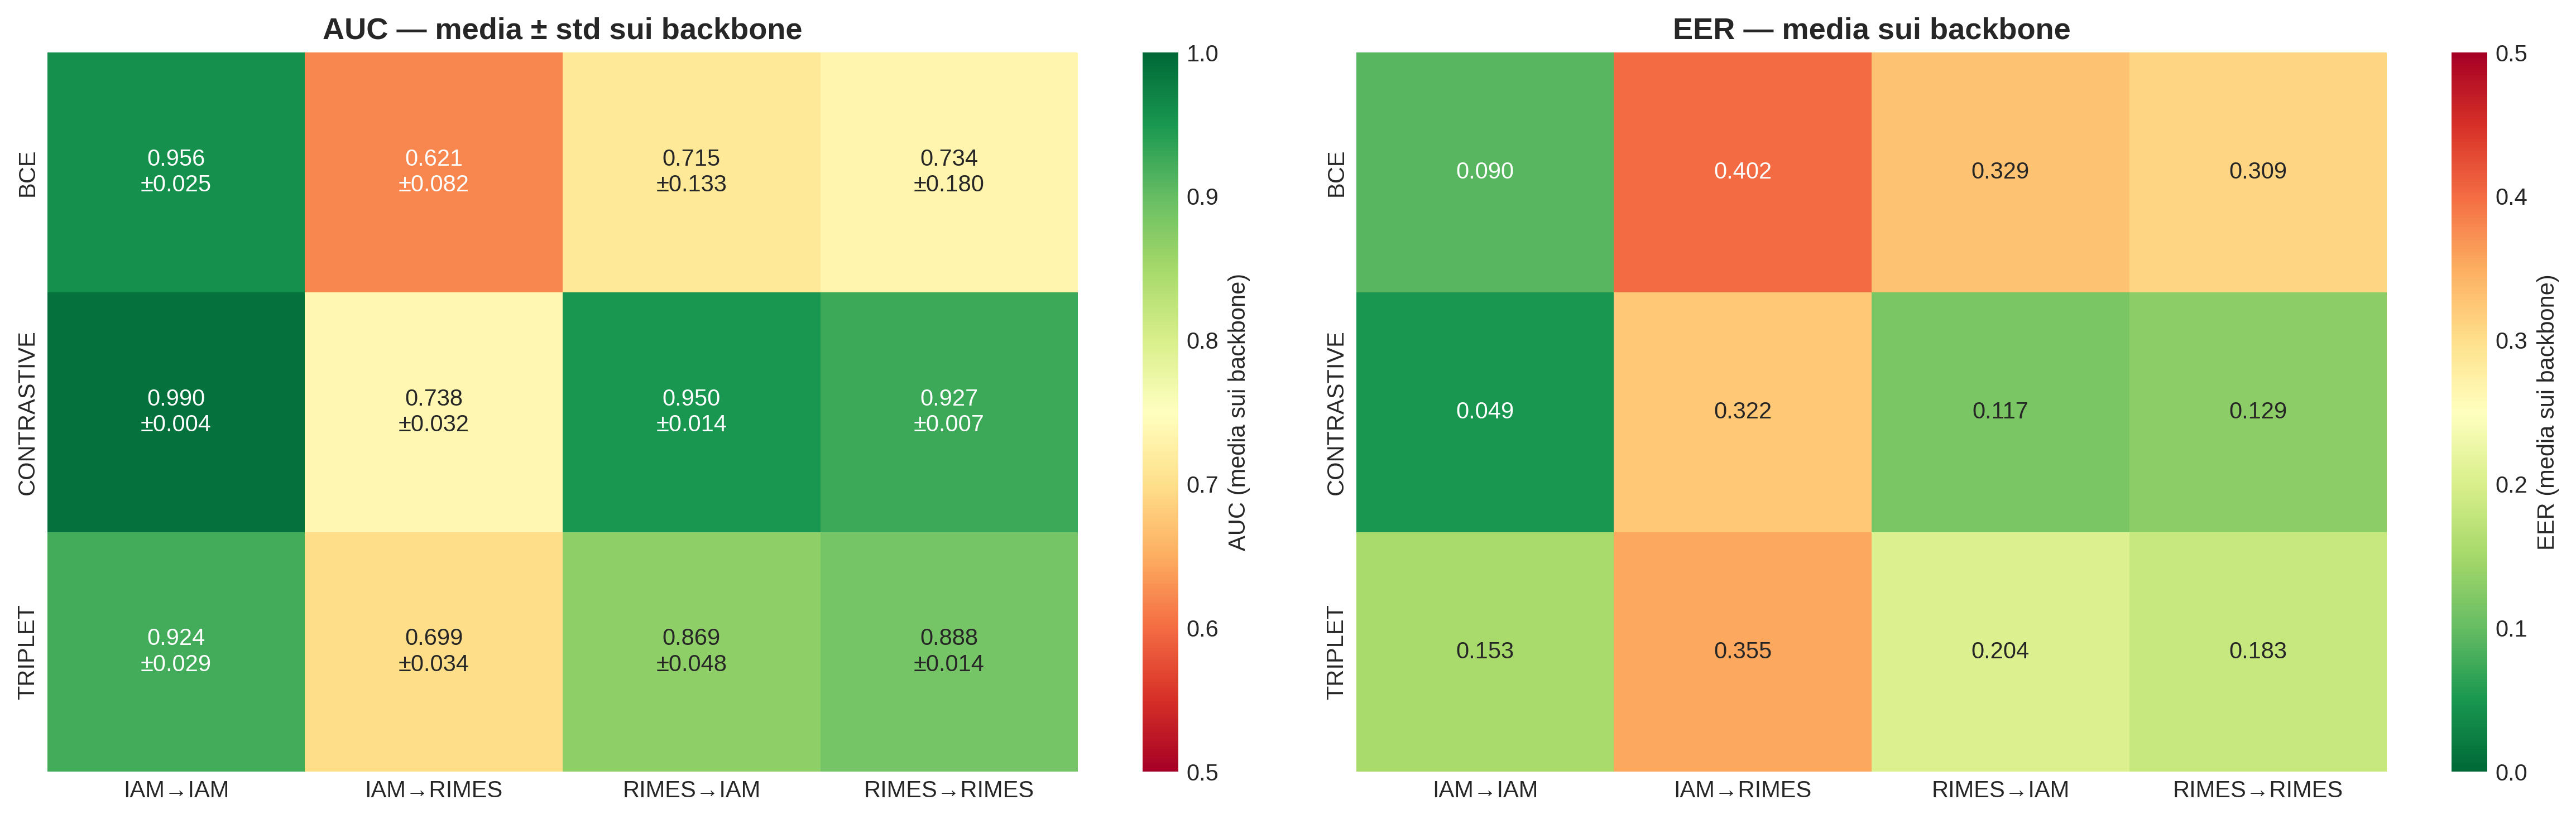
\includegraphics[width=\textwidth]{images/metrics_heatmap_aggregated.png}
  \caption{AUC and EER, mean across the 6 backbones, per
  loss$\times$split combination.}
  \label{fig:heatmap-aggregated}
\end{figure}

Figure~\ref{fig:heatmap-aggregated}: across-backbone AUC std is tight
under Contrastive throughout ($\pm0.004$--$\pm0.032$) but large under
BCE on the two splits with collapsed models (RIMES$\to$RIMES
$\pm0.180$, RIMES$\to$IAM $\pm0.133$). IAM$\to$RIMES is the hardest
cell under every loss (AUC $\leq0.738$); RIMES$\to$IAM under
Contrastive (AUC $0.950$) is close to same-dataset RIMES$\to$RIMES
($0.927$) despite being cross-dataset.

\textbf{Aggregate profile across all losses and splits.}

\begin{table}[htbp]
  \centering
  \caption{Per-backbone verification metrics, averaged across all 12
  loss$\times$split combinations.}
  \label{tab:radar-values}
  \small
  \begin{tabular}{lccccc}
    \toprule
    Backbone & AUC & EER (\%) & $d'$ & GAR@FAR1\% & GAR@FAR0.1\% \\
    \midrule
    ResNet-18            & \textbf{0.869} & \textbf{19.2} & \textbf{1.84} & 9.8\%  & 23.3\% \\
    EfficientNet-B0      & 0.849 & 20.2 & 1.75 & 10.0\% & 25.3\% \\
    EfficientNet-B1      & 0.838 & 21.1 & 1.77 & 14.3\% & \textbf{31.0\%} \\
    MobileNetV3-Large    & 0.833 & 22.3 & 1.59 & 13.1\% & 27.1\% \\
    ResNet-34            & 0.828 & 23.1 & 1.52 & 9.8\%  & 20.2\% \\
    MobileNetV3-Small    & 0.788 & 26.3 & 1.38 & \textbf{14.8\%} & 25.0\% \\
    \bottomrule
  \end{tabular}
\end{table}

\begin{figure}[htbp]
  \centering
  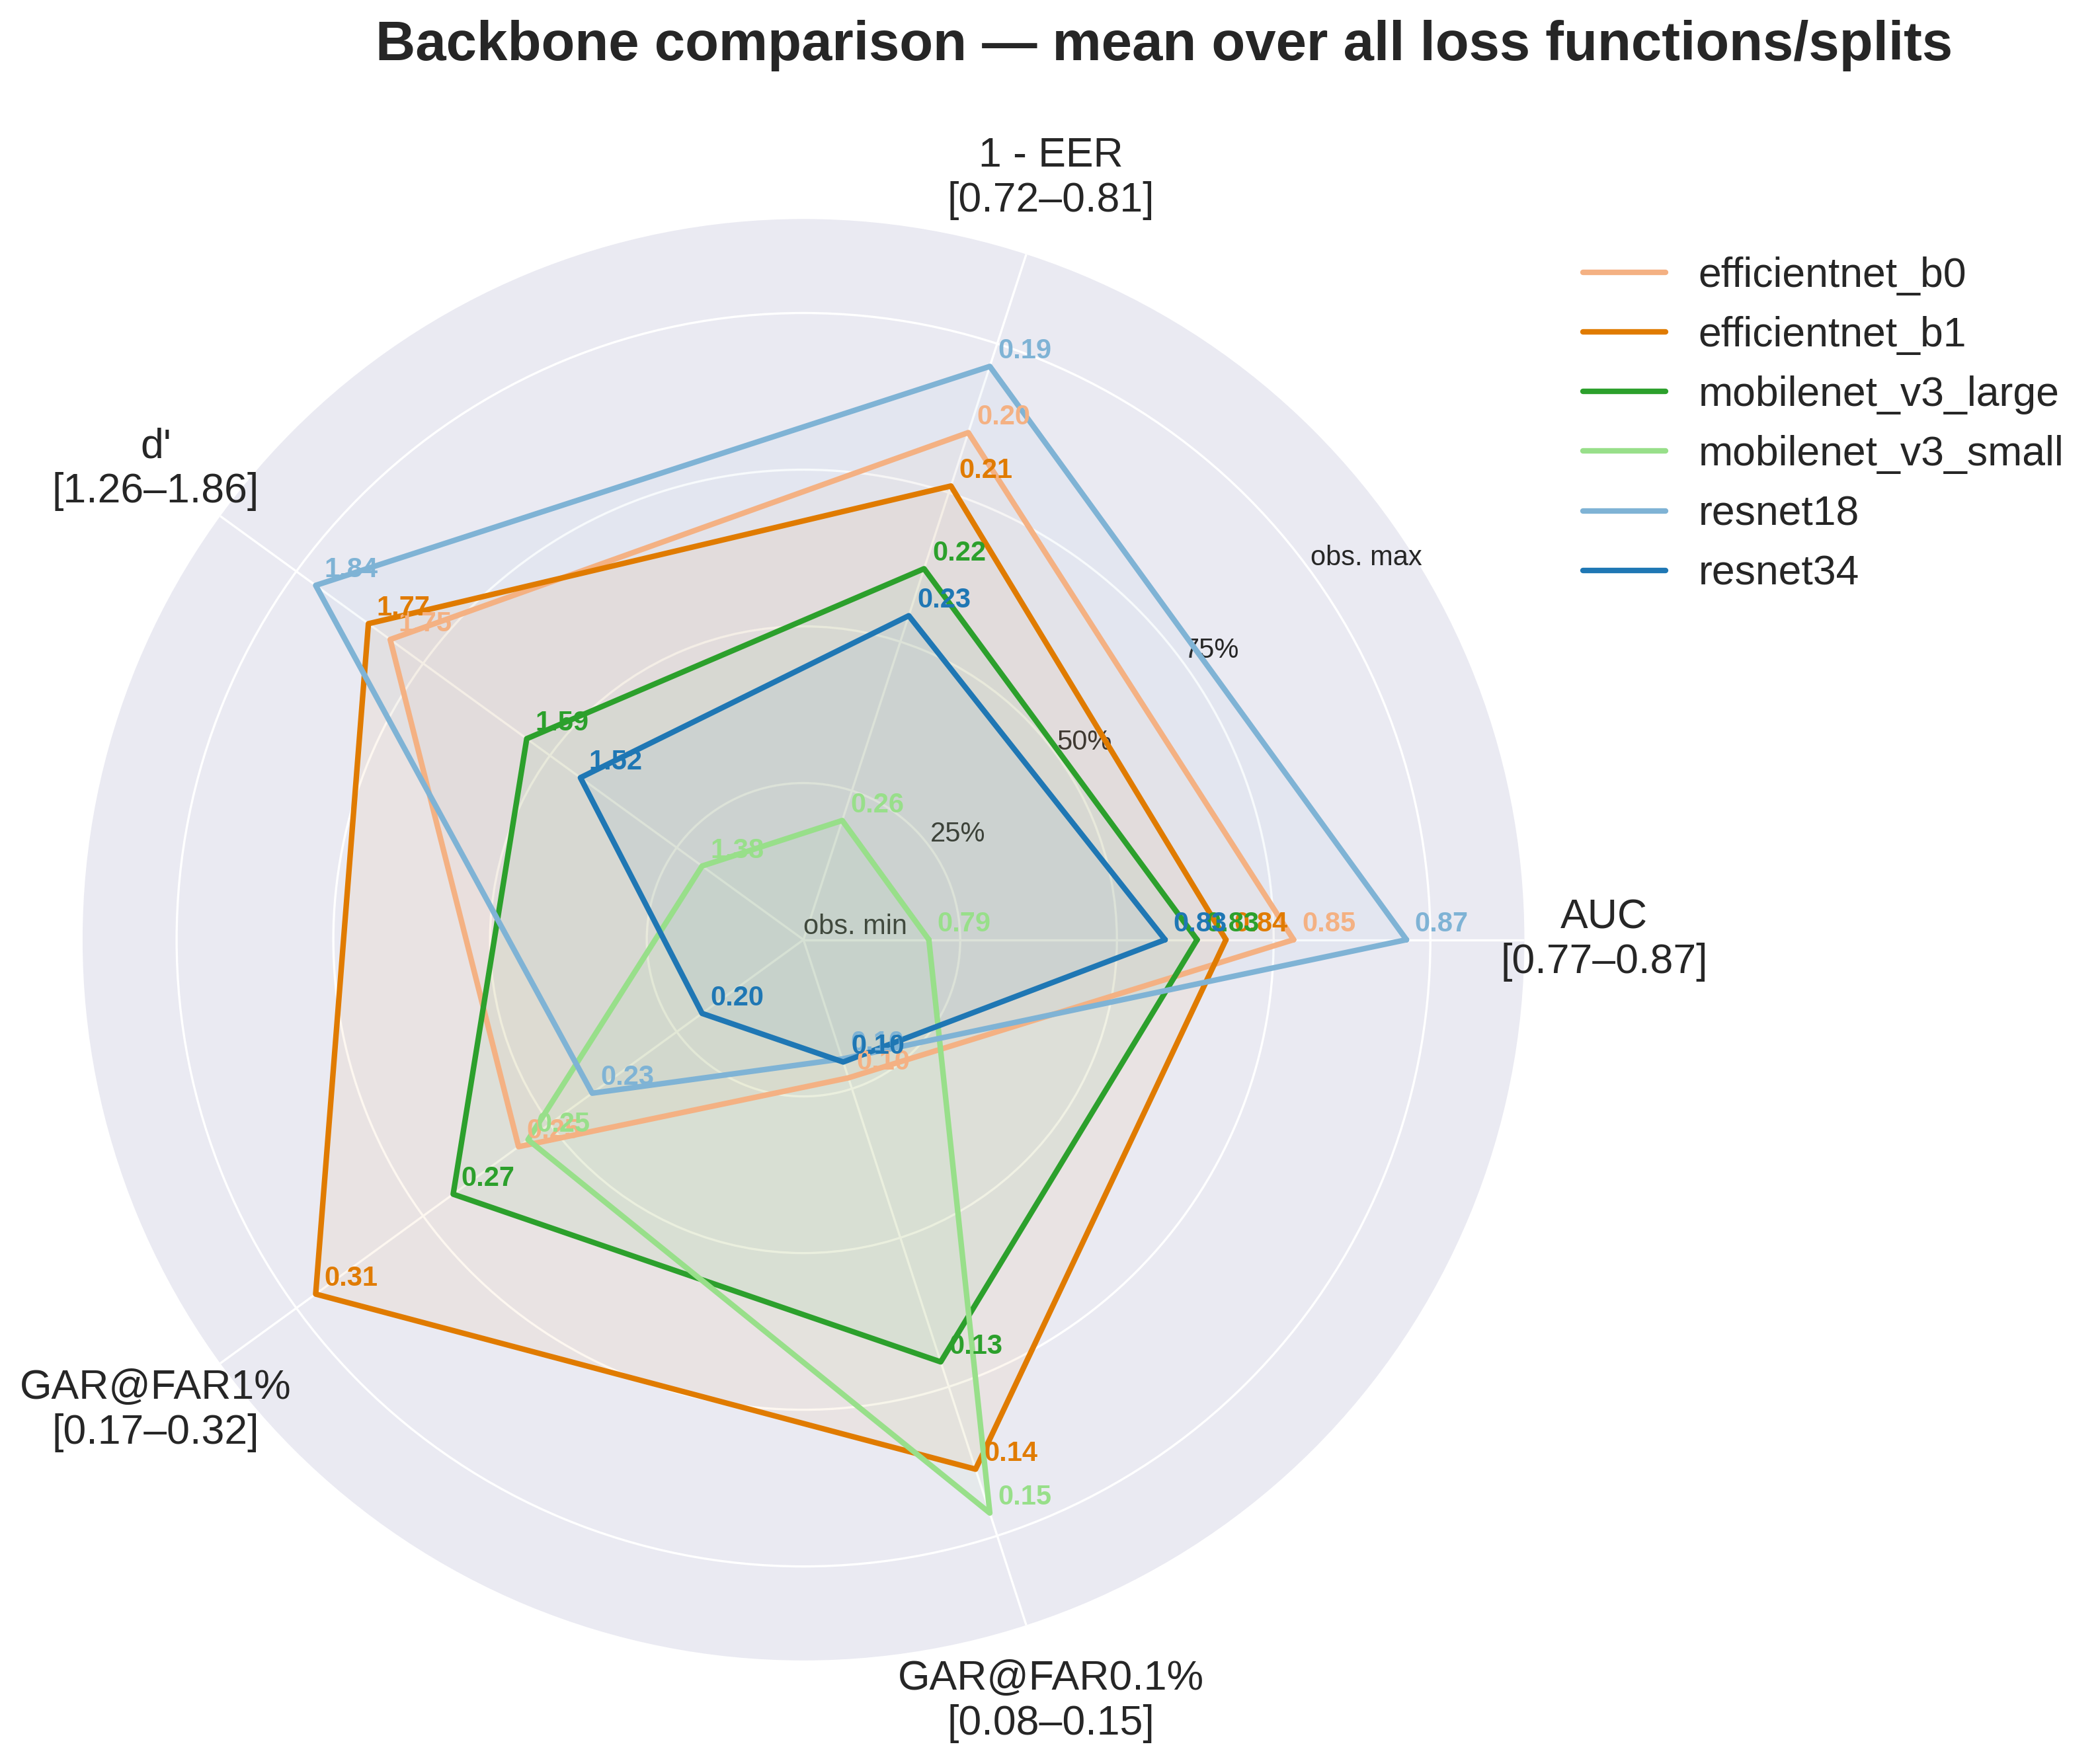
\includegraphics[width=0.75\textwidth]{images/radar_backbone_comparison.png}
  \caption{Per-backbone verification profile, averaged across all loss
  functions and dataset splits. Axis ranges scaled between observed
  min/max per metric; annotated values are raw means
  (Table~\ref{tab:radar-values}). Color by architecture family (blue:
  ResNet, orange: EfficientNet, green: MobileNetV3), darker shade =
  larger variant.}
  \label{fig:radar-backbone}
\end{figure}

ResNet-18 ranks first on AUC, EER and $d'$, but has the lowest
GAR@FAR1\% (9.8\%) and second-lowest GAR@FAR0.1\% (23.3\%) of all six
backbones. Overall separability and low-FAR-tail behavior are
therefore decoupled for this backbone: a small number of
high-scoring impostor pairs depresses GAR at strict thresholds without
affecting AUC/EER, consistent with the boundary-saturated impostor
tail reported for ResNet-18 under Contrastive on cross-dataset splits
(Section~\ref{sec:failure-analysis}).

EfficientNet-B1 shows the inverse profile: fourth on AUC, third on
EER/$d'$, but highest GAR@FAR0.1\% (31.0\%, $+7.7$ points over
ResNet-18).

MobileNetV3-Small has the worst AUC, EER and $d'$ of all six backbones,
consistent with its two collapsed BCE configurations, yet the highest
GAR@FAR1\% (14.8\%) — an isolated-threshold effect, not a
discriminability advantage.

Within the ResNet family, ResNet-34 underperforms ResNet-18 on every
metric except GAR@FAR1\% (near-tied, 9.8\% vs.\ 9.8\%), despite twice
the parameter count; no comparable inversion occurs between
EfficientNet-B0/B1. ResNet-34 is the only backbone that leads on no
metric in Table~\ref{tab:radar-values}.

Taken together, these results lead us to select ResNet-18 as the backbone for the subsequent analyses.


\subsection{Paired analysis of loss-function performance}
\label{sec:significance}

\begin{table}[htbp]
  \centering
  \caption{Paired Wilcoxon signed-rank test on AUC ($n=24$: 6 backbones
  $\times$ 4 splits).}
  \label{tab:wilcoxon}
  \begin{tabular}{lccccc}
    \toprule
    Comparison & Mean AUC (A) & Mean AUC (B) & $W$ & $p$ & Effect size \\
    \midrule
    BCE vs.\ Contrastive     & 0.756 & 0.901 & 1.0  & $2.38\times10^{-7}$ & $-0.993$ \\
    BCE vs.\ Triplet         & 0.756 & 0.845 & 63.0 & $0.0115$             & $-0.580$ \\
    Contrastive vs.\ Triplet & 0.901 & 0.845 & 0.0  & $1.19\times10^{-7}$ & $+1.000$ \\
    \bottomrule
  \end{tabular}
\end{table}

Because the 24 observations are not fully independent experimental replicates---they share the same backbone architectures, dataset splits, and underlying data, and each configuration is represented by a single training run---the Wilcoxon tests are interpreted as paired analyses of the consistency of loss-function differences across configurations, rather than as evidence from 24 independent training experiments. Under this interpretation, all three pairwise comparisons are statistically significant at $\alpha=0.05$. Contrastive significantly outperforms both BCE and Triplet, with very large effect sizes ($\rho=-0.993$ and $\rho=+1.000$, respectively; both $p<10^{-6}$). Triplet also outperforms BCE, although the effect is substantially smaller ($\rho=-0.580$, $p=0.0115$). Since the training recipes are uniform across losses (Section~\ref{subsubsec:dataset-pairings}), these differences are consistent with an effect of the loss objective itself. However, as discussed in Section~\ref{sec:per-backbone}, Contrastive's overall advantage does not necessarily reflect a uniform improvement across all architectures; part of its gain arises from its greater robustness on architectures for which BCE exhibits higher variability.

\subsection{High-precision validation with an exhaustive impostor pool}
\label{sec:exhaustive}

For ResNet-18 + Contrastive trained on RIMES and evaluated on the
\emph{full} IAM impostor pool (4{,}051 genuine pairs against
1{,}179{,}440 impostor pairs, $\sim\!291\times$ the balanced
protocol's impostor count), the exhaustive-pool re-evaluation gives:

\begin{table}[htbp]
  \centering
  \caption{Exhaustive-impostor-pool validation, RIMES$\to$IAM,
  ResNet-18 + Contrastive, vs.\ the balanced protocol.}
  \label{tab:exhaustive}
  \small
  \begin{tabular}{lcccc}
    \toprule
    Protocol & Impostor pairs & AUC & EER & GAR@1\% \\
    \midrule
    Balanced   & 4{,}051       & 0.967 & 8.2\%  & 62.6\% \\
    Exhaustive & 1{,}179{,}440 & 0.945 & 13.0\% & 34.5\% \\
    \bottomrule
  \end{tabular}
\end{table}

The exhaustive pool shows a genuine, non-trivial degradation relative
to the balanced protocol (AUC $0.967\to0.945$; EER $8.2\%\to13.0\%$;
GAR@1\% $62.6\%\to34.5\%$), indicating that 1:1 balanced impostor
subsampling in the main sweep was moderately optimistic for this
configuration. This is run for a single (backbone, loss, split) triple
only, given the cost of exhaustive scoring, and does not revisit the
per-backbone (Section~\ref{sec:per-backbone}) or Wilcoxon
(Section~\ref{sec:significance}) analyses.

\subsection{Best-model summary}
\label{sec:roc-det}

\begin{table}[htbp]
  \centering
  \caption{Best-performing (backbone, loss) configuration per split
  (Table~4).}
  \label{tab:ours-best}
  \small
  \begin{tabular}{llcc}
    \toprule
    Split & Best (backbone, loss) & AUC & EER \\
    \midrule
    IAM$\to$IAM     & MobileNetV3-Large, Contrastive & 0.995 & 3.1\%  \\
    IAM$\to$RIMES   & EfficientNet-B1, Contrastive   & 0.772 & 29.6\% \\
    RIMES$\to$IAM   & EfficientNet-B0, Contrastive   & 0.967 & 8.2\%  \\
    RIMES$\to$RIMES & ResNet-18, Contrastive         & 0.934 & 11.5\% \\
    \bottomrule
  \end{tabular}
\end{table}

\begin{table}[htbp]
  \centering
  \caption{Classification metrics at the EER threshold, best
  (backbone, loss) per split (Table~4).}
  \label{tab:classification-metrics}
  \small
  \begin{tabular}{lcccccc}
    \toprule
    Split & Accuracy & Precision & Recall & F1 & $\mu_g/\mu_i$ & $\sigma_g/\sigma_i$ \\
    \midrule
    IAM$\to$IAM     & 0.969 & 0.969 & 0.969 & 0.969 & 0.893/0.005 & 0.118/0.277 \\
    IAM$\to$RIMES   & 0.704 & 0.704 & 0.704 & 0.704 & 0.829/0.648 & 0.170/0.219 \\
    RIMES$\to$IAM   & 0.918 & 0.918 & 0.918 & 0.918 & 0.938/0.413 & 0.110/0.294 \\
    RIMES$\to$RIMES & 0.885 & 0.885 & 0.885 & 0.885 & 0.791/0.063 & 0.284/0.357 \\
    \bottomrule
  \end{tabular}
\end{table}

As noted in Section~\ref{sec:protocol}, these figures are computed at
the EER threshold of each model on its own evaluation set, not an
independently calibrated threshold. The provided ROC/DET/distribution
figures (Figures~\ref{fig:roc}--\ref{fig:distributions}) cover
ResNet-18 across all 12 loss$\times$split combinations, and are shown
as a representative supplementary panel rather than as the
aggregate-best-per-split configurations of
Table~\ref{tab:ours-best} (which include MobileNetV3-Large and
EfficientNet-B0/B1 for three of the four splits).

\begin{figure}[htbp]
  \centering
  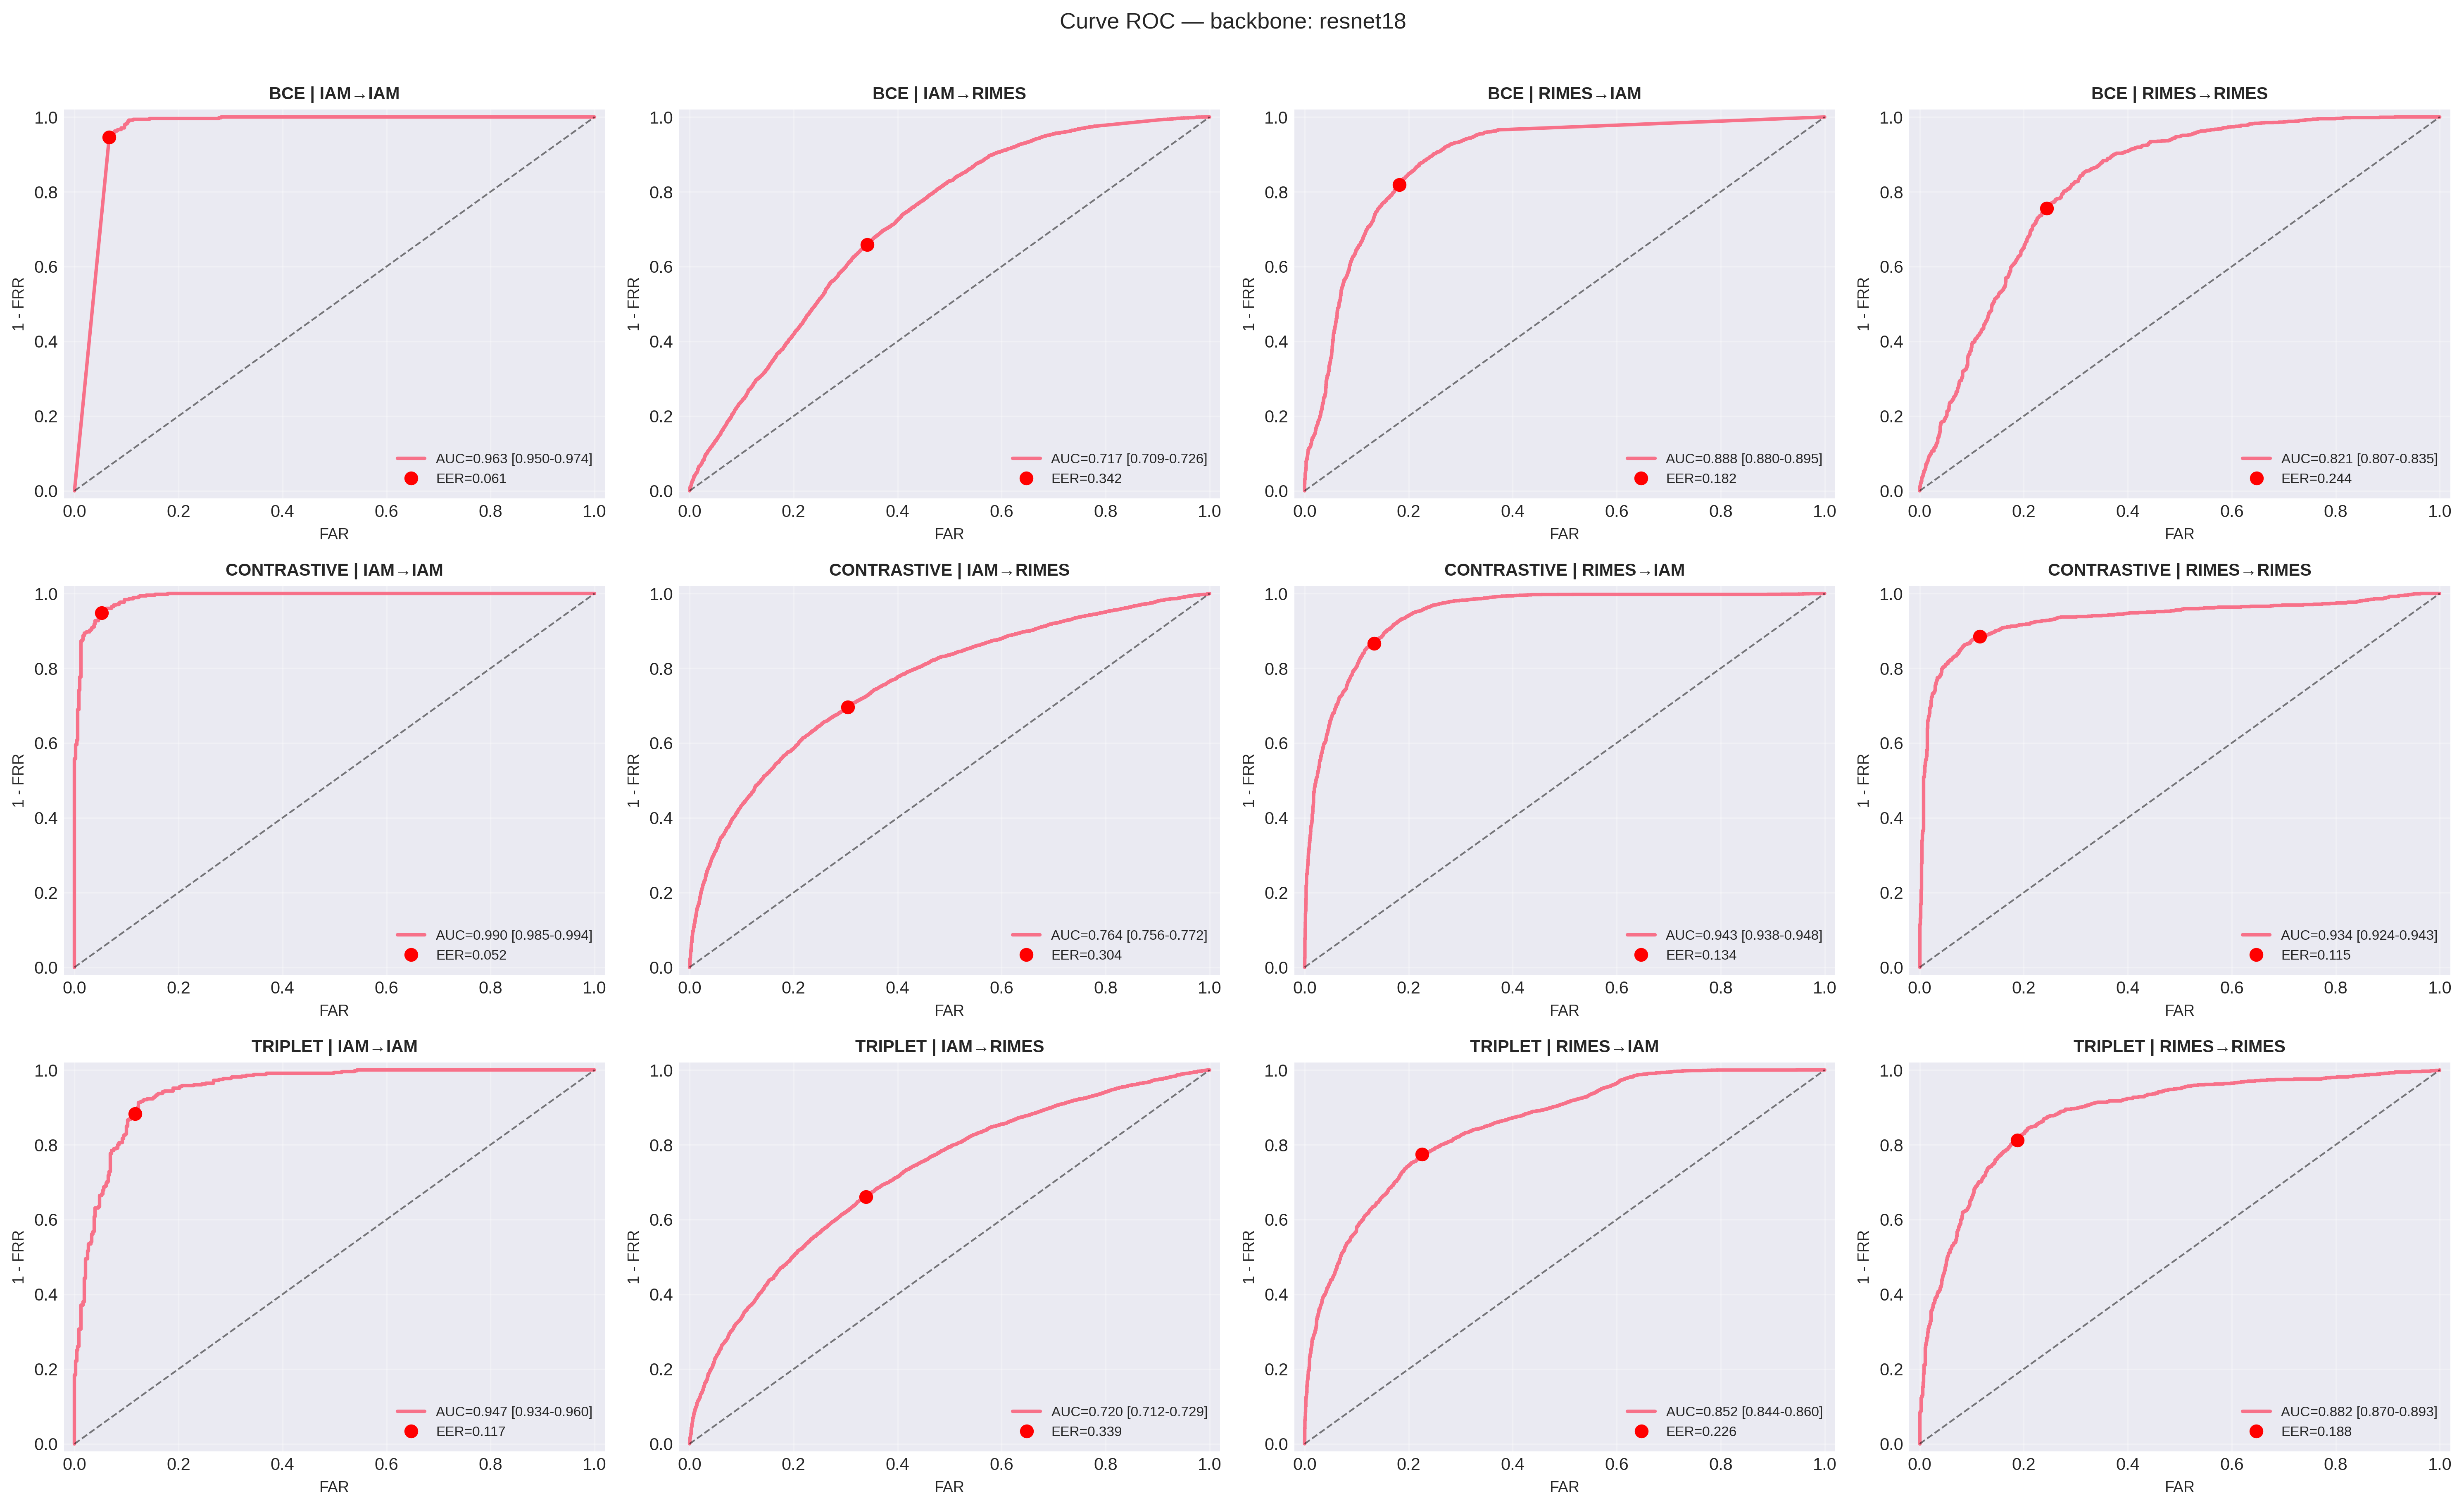
\includegraphics[width=\textwidth]{images/roc_curves_resnet18.png}
  \caption{ROC curves, ResNet-18, all losses/splits.
  Bootstrap 95\% confidence intervals for AUC are reported in each
  panel legend.}
  \label{fig:roc}
\end{figure}

The ROC curves in Figure~\ref{fig:roc} report bootstrap 95\%
confidence intervals alongside each AUC estimate. Contrastive
achieves the highest AUC on all four splits for ResNet-18 (IAM$\to$IAM:
0.990; IAM$\to$RIMES: 0.764; RIMES$\to$IAM: 0.943; RIMES$\to$RIMES:
0.934), consistently outperforming BCE and Triplet across the full
FAR range rather than only near the EER operating point. The ordering
of BCE and Triplet is not fixed across splits: BCE outperforms Triplet
on two of the four splits (IAM$\to$IAM, RIMES$\to$IAM,), but Triplet marginally exceeds BCE on IAM$\to$RIMES, the hardest cross-dataset pairing for this
backbone, and RIMES$\to$RIMES. Confidence-interval width is governed primarily by
evaluation-set size rather than by the same-vs-cross-dataset
distinction: the narrowest interval overall belongs to
Contrastive/IAM$\to$IAM (width $0.009$, $n=958$ pairs), while
BCE/IAM$\to$IAM and BCE/RIMES$\to$RIMES -- despite being a same-dataset split -- shows the widest intervals (width $0.024$ and $0.028$, respectively), reflecting their comparatively
small test sets relative to the cross-dataset splits (e.g.\
IAM$\to$RIMES, $n=12{,}858$ pairs, CI width $0.016$--$0.017$ across
losses). At the shape level, the same-dataset curves (IAM$\to$IAM,
RIMES$\to$RIMES) rise sharply toward the top-left corner across all
three losses, whereas the cross-dataset curves -- particularly
IAM$\to$RIMES -- remain comparatively close to the chance diagonal
over a wide FAR range, visually corroborating the same-vs-cross-dataset
generalization gap discussed in Section~\ref{sec:cross-dataset}.

\begin{figure}[htbp]
  \centering
  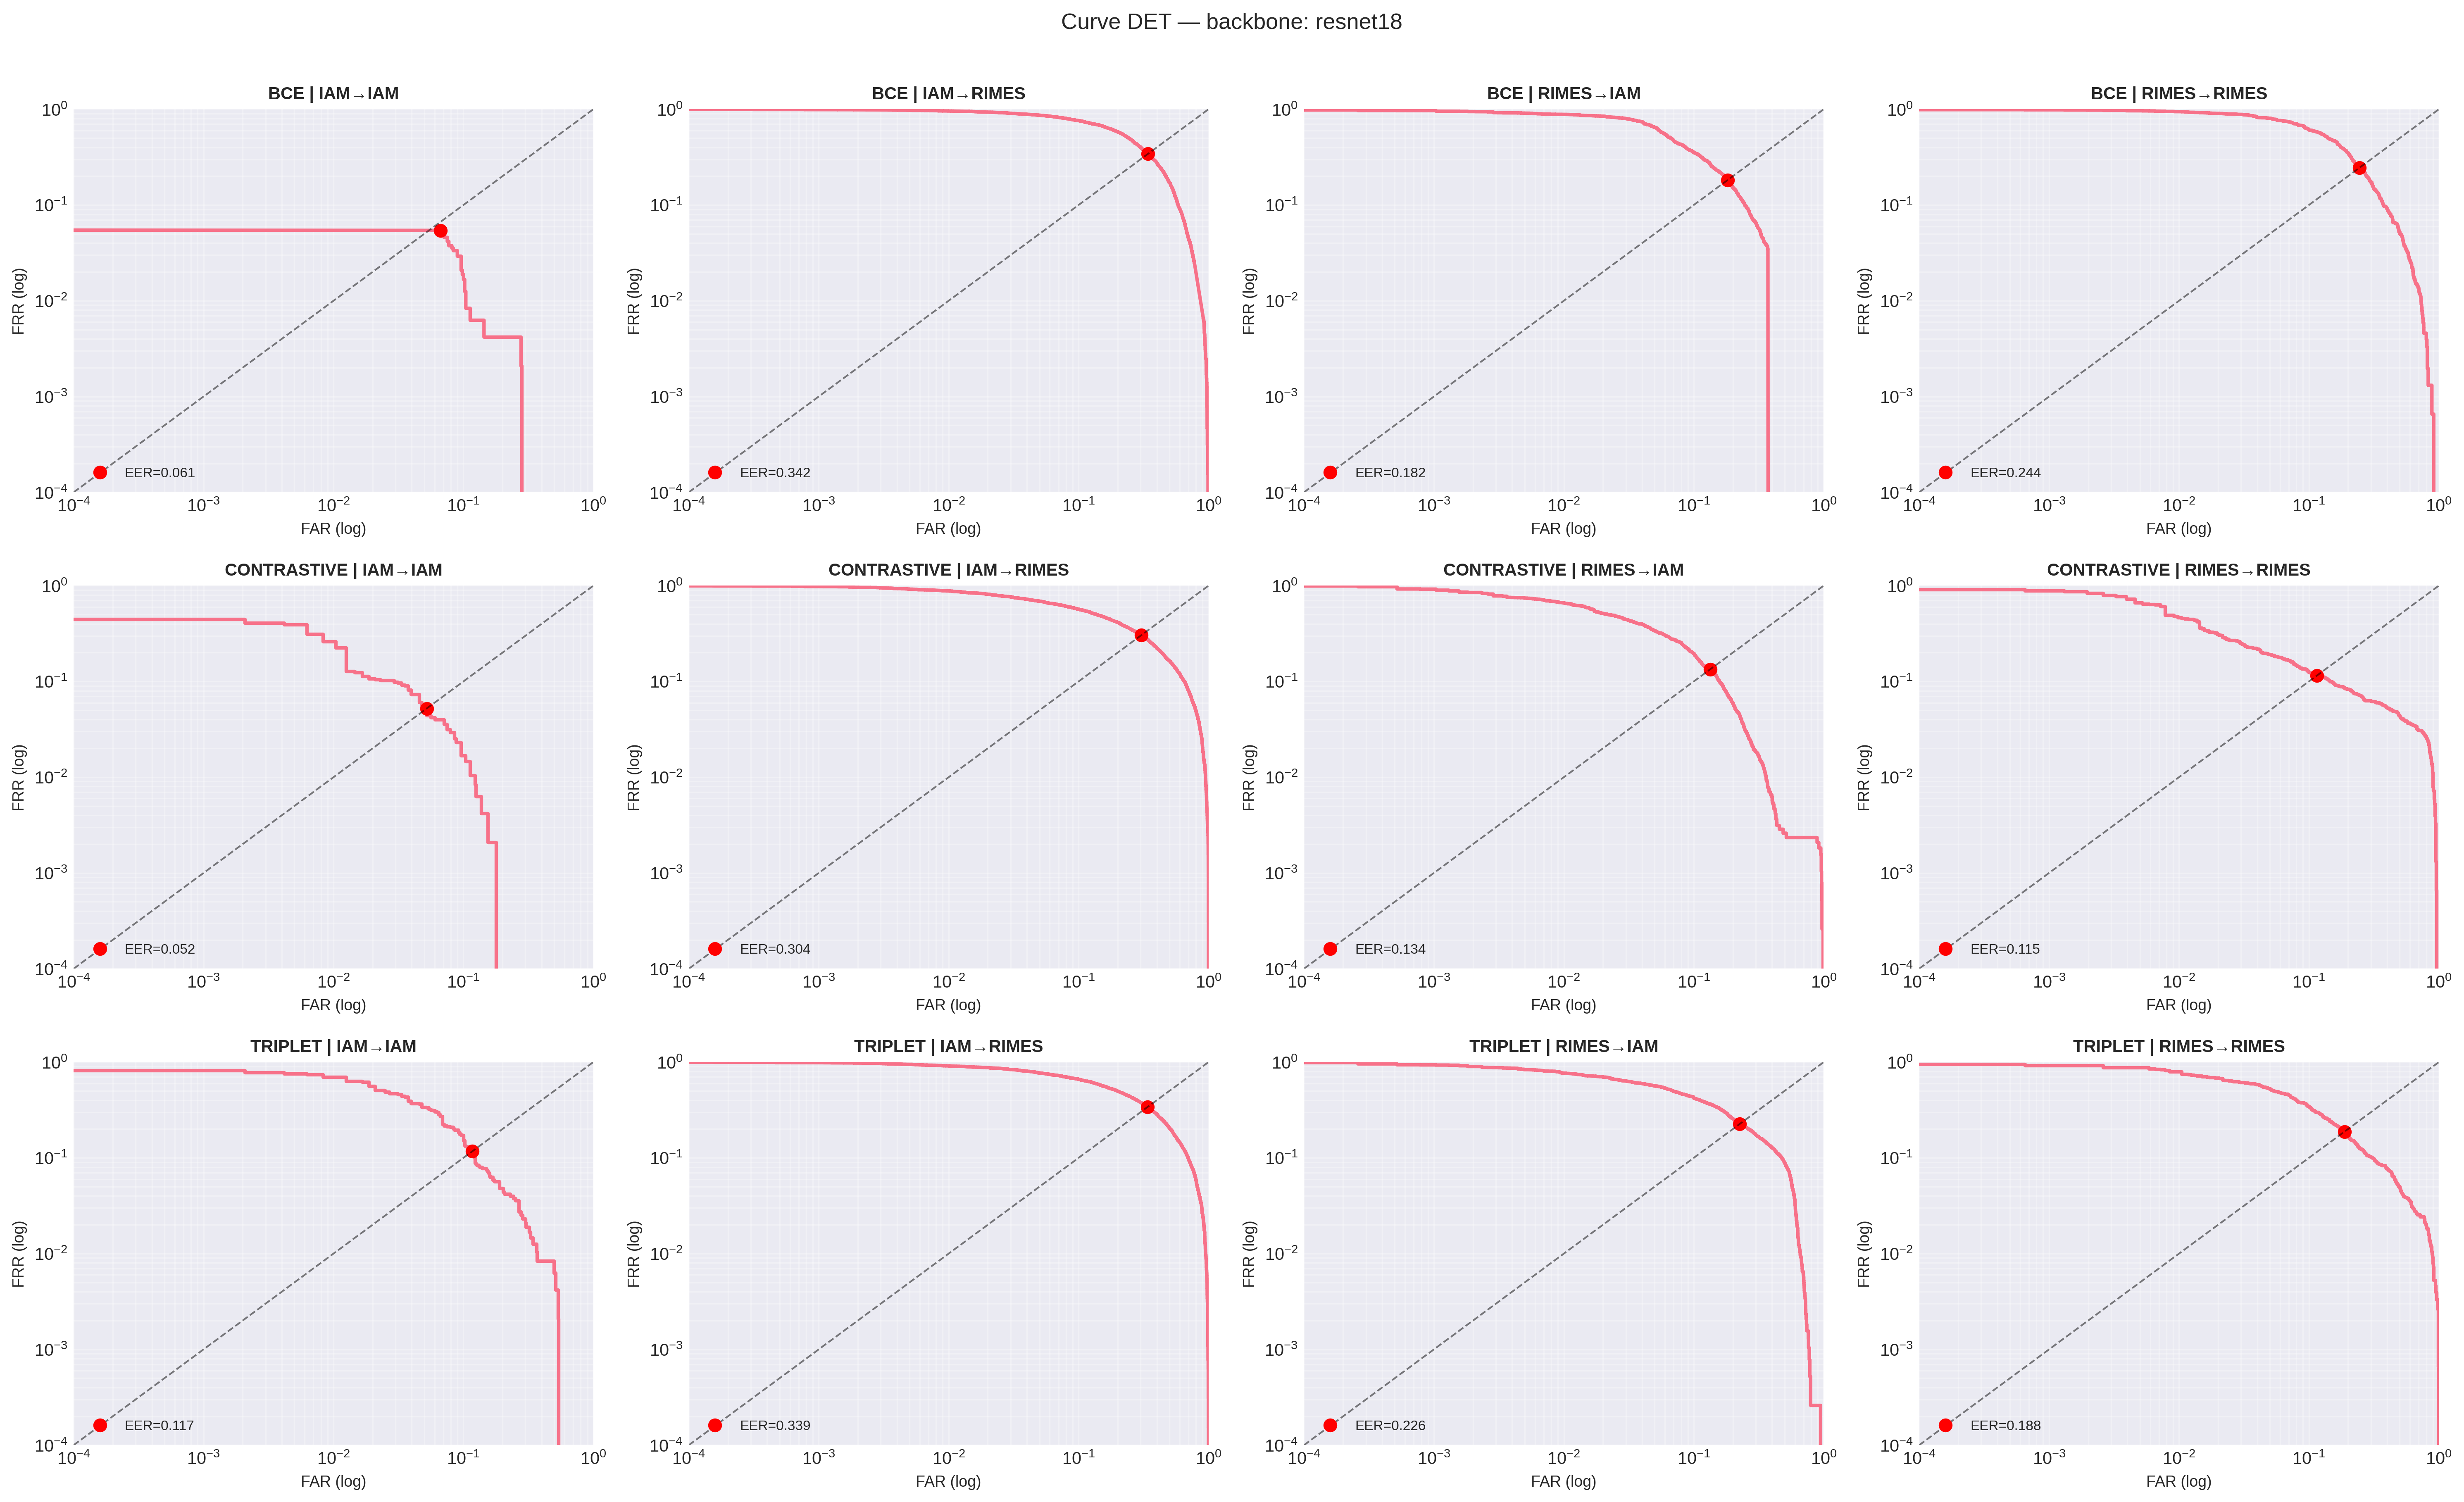
\includegraphics[width=\textwidth]{images/det_curves_resnet18.png}
  \caption{DET curves (log-log), ResNet-18, all losses/splits
  (supplementary).}
  \label{fig:det}
\end{figure}

The DET curves in Figure~\ref{fig:det} provide a visual representation
of the strong variation in verification performance across losses and
dataset splits. The IAM$\to$IAM curves are consistently the most
favorable, reaching relatively low FRR at small FAR values across all
three losses. However, the shape differs by loss: BCE exhibits a
pronounced, nearly flat plateau in the low-FAR region before dropping
sharply, Contrastive shows a comparable but noisier and less
perfectly flat shelf at a higher FRR level, while Triplet decreases
more smoothly and monotonically without a distinct plateau. In
contrast, the IAM$\to$RIMES curves remain close to the upper part of
the plot over a large portion of the FAR range for all three losses,
indicating a substantial loss of discrimination under the
cross-dataset shift, with a sharp drop only near each curve's EER
point. RIMES$\to$IAM shows intermediate behavior between the two
same-dataset splits and IAM$\to$RIMES, with Contrastive (EER $=13.4\%$)
clearly outperforming BCE (EER $=18.2\%$) and Triplet (EER $=22.6\%$).
The RIMES$\to$RIMES curves, evaluated on the second same-dataset
split, also show substantial variation across losses, with Contrastive
producing the most favorable operating characteristics and the lowest
EER ($11.5\%$ vs.\ $24.4\%$ for BCE and $18.8\%$ for Triplet). Overall,
the DET plots corroborate the strong dependence of verification
performance on the dataset pairing: the cross-dataset shift is
particularly detrimental for IAM$\to$RIMES, where all three losses
exhibit substantially higher FRR across the operating range than in
either same-dataset setting. Among the two cross-dataset splits,
Contrastive provides the more favorable behavior on RIMES$\to$IAM,
although its performance still degrades markedly relative to its own
same-dataset results under the IAM$\to$RIMES shift.

\subsection{Score distributions and the Gaussianity assumption}
\label{sec:distributions}

Shapiro--Wilk tests on all 72 genuine and 72 impostor score
distributions reject normality universally at $\alpha=0.05$ (largest
observed $p$-value $\sim2\times10^{-6}$, ResNet-18/Contrastive/RIMES$\to$RIMES
genuine scores); no distribution in the sweep is Gaussian-compatible.
Consequently, $d'$/decidability are reported throughout this paper
strictly as descriptive, rank-consistent indices rather than as
parametric inferential statistics.

\begin{figure}[htbp]
  \centering
  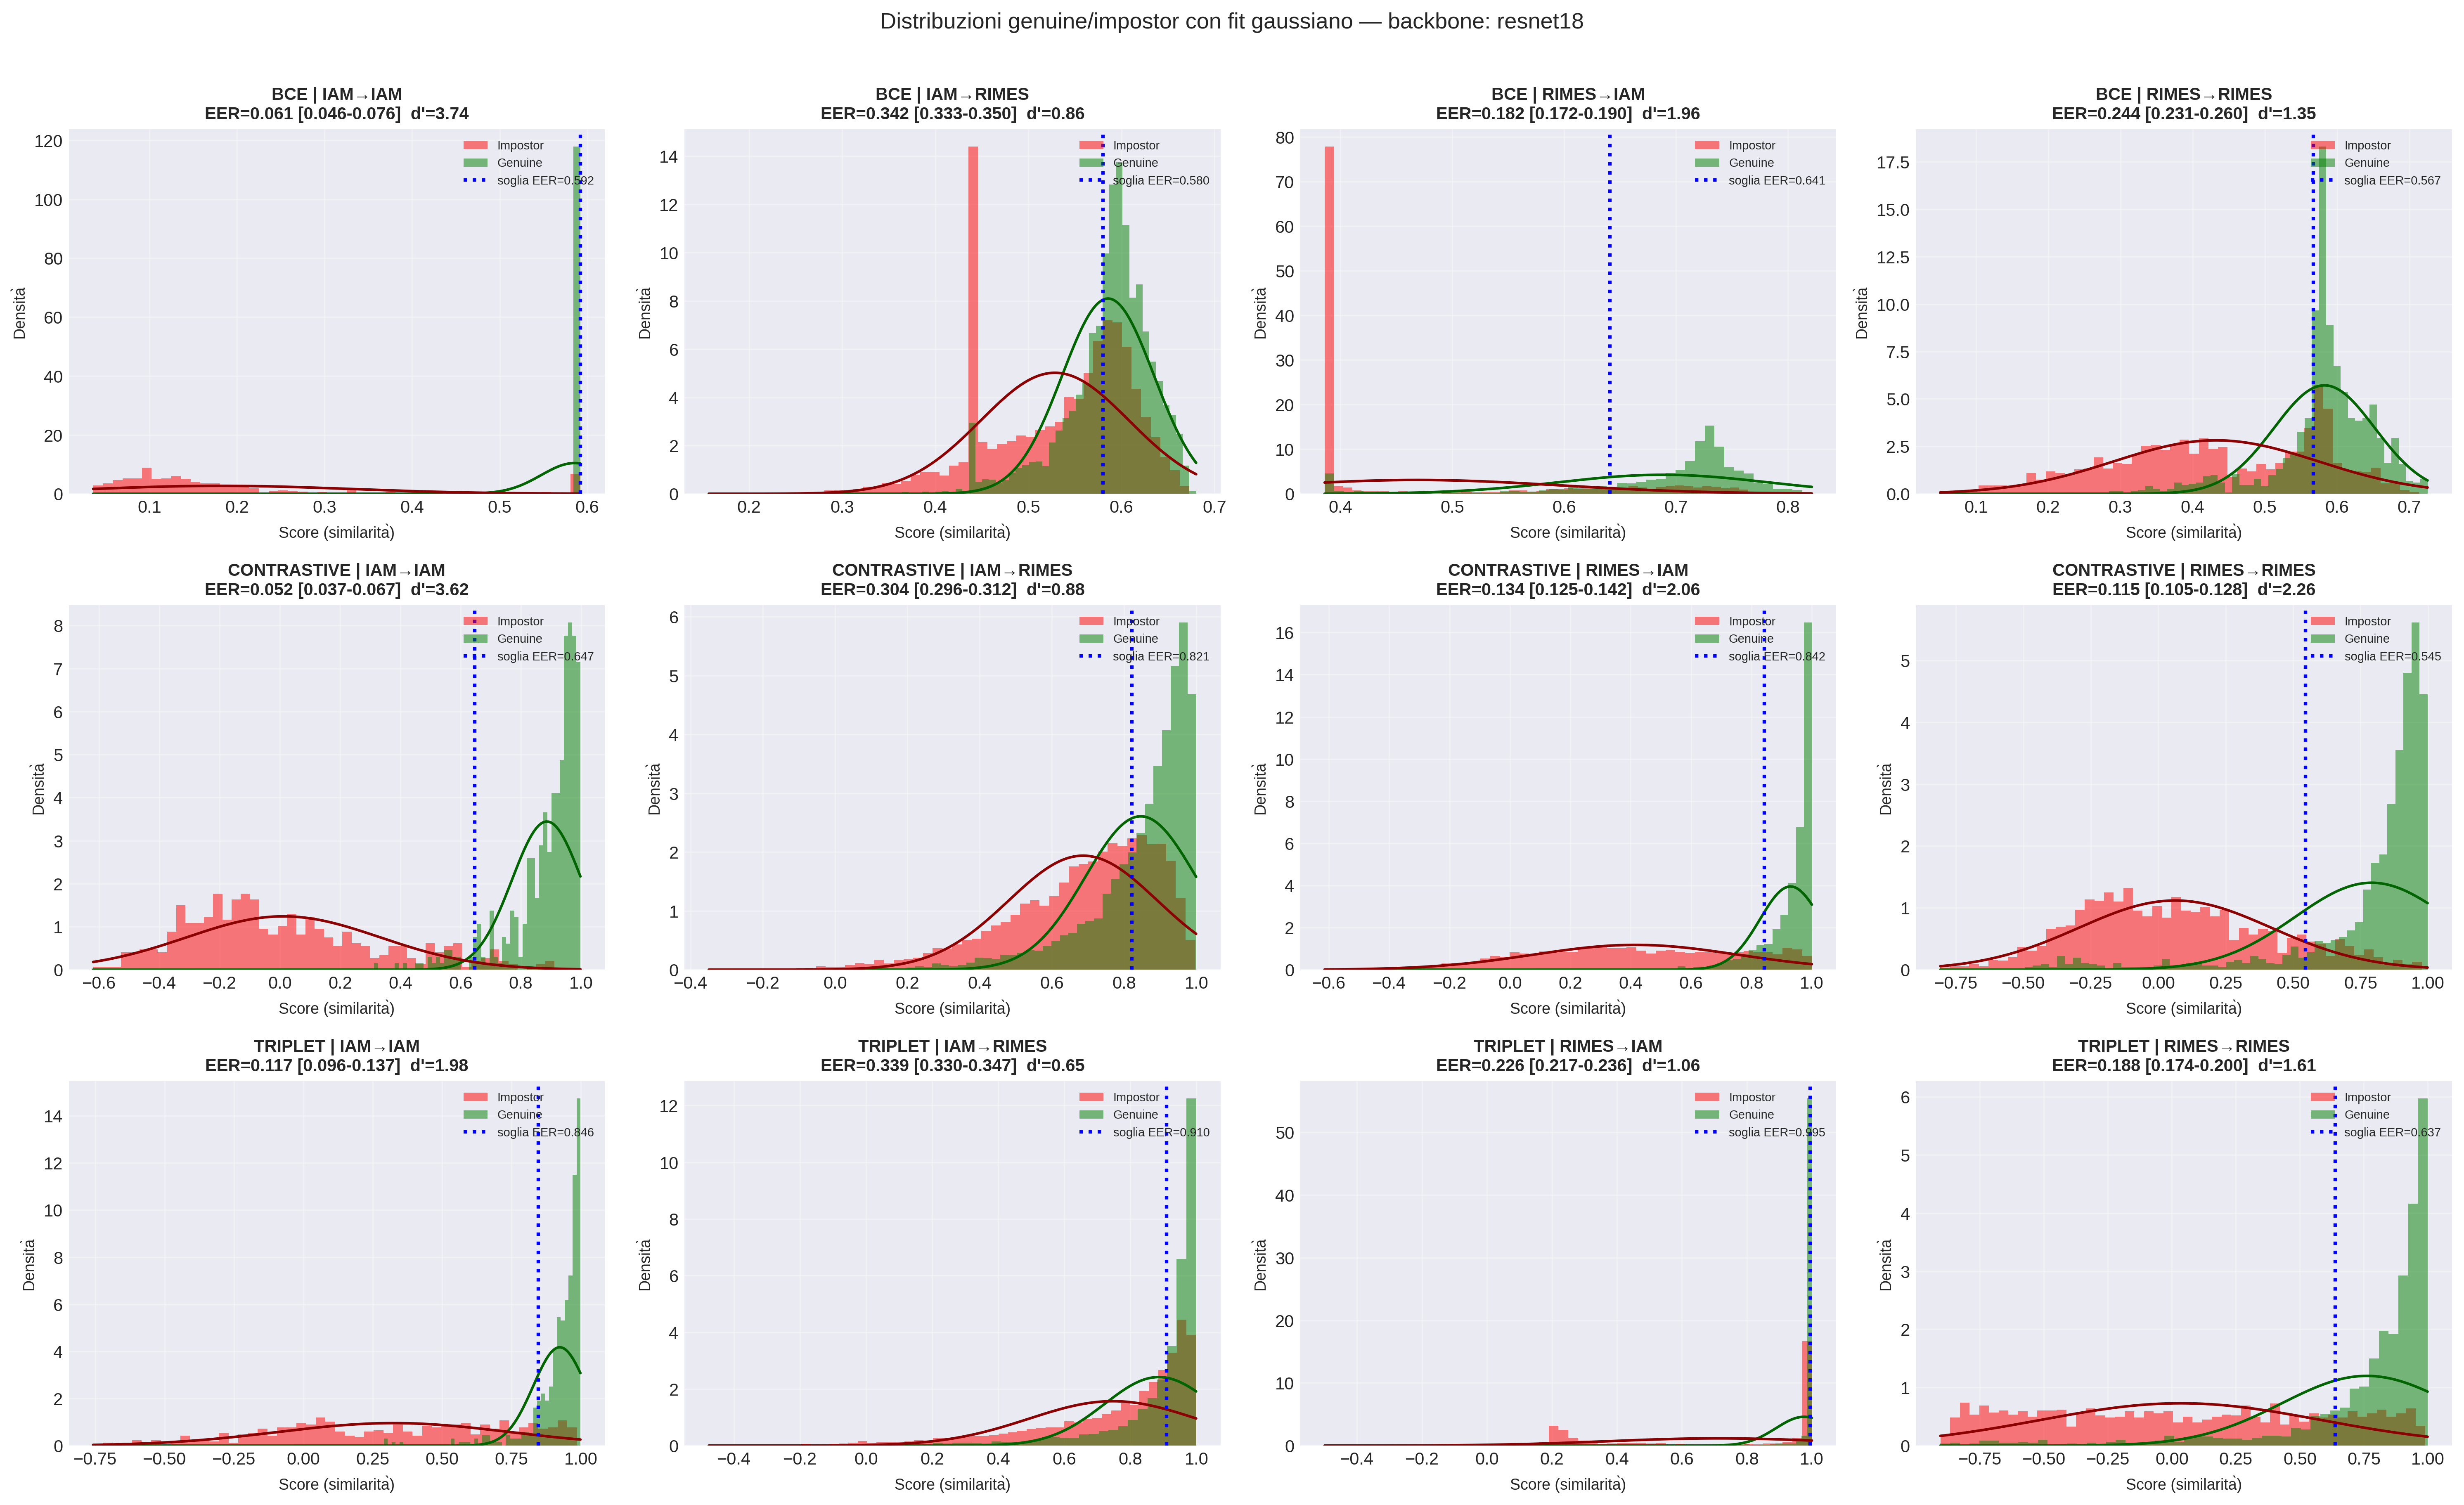
\includegraphics[width=\textwidth]{images/score_distributions_resnet18.png}
  \caption{Genuine (green)/impostor (red) scores with fitted Gaussian
  overlays, ResNet-18, all loss$\times$split combinations. Dotted
  lines: EER threshold. None of the 12 distributions shown pass
  Shapiro--Wilk at $\alpha=0.05$.}
  \label{fig:distributions}
\end{figure}

Visual inspection of Figure~\ref{fig:distributions} shows that
BCE/RIMES$\to$IAM and BCE/RIMES$\to$RIMES exhibit substantially more
genuine-impostor overlap than the same-dataset IAM$\to$IAM panel,
consistent with their comparatively higher EER ($18.2\%$ and $24.4\%$,
respectively, vs.\ $6.1\%$ for BCE/IAM$\to$IAM); this reflects a
genuine loss of separability under BCE on these splits, though for
ResNet-18 both configurations remain well above chance-level
discrimination (AUC $=0.888$ and $0.821$; ResNet-18 does not exhibit
any of the fully collapsed, near-chance BCE configurations documented
for other backbones in Section~\ref{sec:per-backbone}). Contrastive
and Triplet distributions, by contrast, display visible
boundary-clustered mass near the similarity limits $\pm 1$,
particularly for RIMES$\to$IAM.

A further pattern visible in Figure~\ref{fig:distributions} is that
under BCE, several impostor distributions exhibit a narrow, isolated
spike at a fixed low score (e.g.\ BCE/RIMES$\to$IAM, impostor mass
concentrated near score $\approx 0.39$; BCE/IAM$\to$RIMES, near
$\approx 0.44$), rather than a smooth unimodal shape -- a possible
signature of a degenerate embedding direction rather than genuine
score variability. Under Contrastive and Triplet, by contrast,
impostor distributions are broad and (generally) left-skewed while genuine
distributions are (gnerally) right-skewed and compressed near the similarity
ceiling ($\approx 1.0$), producing the asymmetric overlap responsible
for the boundary-saturation effect noted above; this asymmetry is most
pronounced for cross-dataset splits, and least pronounced for same-dataset splits,
mirroring the EER ordering across splits
(Tables~\ref{tab:same-dataset}--\ref{tab:cross-dataset}).

\subsection{Failure-case analysis}
\label{sec:failure-analysis}

We inspect failure modes of the strongest configuration per split
(Table~\ref{tab:ours-best}) using the ResNet-18 distribution plots
(Figure~\ref{fig:distributions}) and, for RIMES$\to$IAM (ResNet-18 +
Contrastive), a pair-level export of the top false accepts and false
rejects.

\begin{itemize}
\item\textbf{Distribution-level patterns.} Two failure modes are visible
for ResNet-18. First, BCE/IAM$\to$RIMES shows genuine and impostor
modes heavily overlapping around the same $0.5$--$0.6$ score region
(EER $=34.2\%$, $d'=0.86$), the weakest separation among all four
BCE panels and the closest ResNet-18 comes to the near-chance behavior
of the fully collapsed models in Section~\ref{sec:per-backbone} (none
of which involve ResNet-18); BCE/RIMES$\to$RIMES shows a milder
version, with a broader impostor distribution encroaching on the
genuine mode's lower tail (EER $=24.4\%$, $d'=1.35$) while the genuine
peak stays distinct. Second, under Contrastive on both cross-dataset
splits, a non-trivial fraction of impostor pairs saturate near the
maximum cosine similarity ($\approx1.0$), overlapping the genuine
mode; this produces the long, shallow DET tail in
Figure~\ref{fig:det} and explains why GAR at strict FAR
(Section~\ref{sec:operating-points}) collapses to single digits on
IAM$\to$RIMES despite a moderate mean EER ($32.2\%$).

\item \textbf{Pair-level inspection (RIMES$\to$IAM, ResNet-18 +
Contrastive).} Figure~\ref{fig:false-accepts} shows the top false
accepts (scores $0.9986$/$0.9964$, $\Delta \approx+0.155$/$+0.154$
above the $0.8424$ threshold): different writers sharing slant,
spacing, and regularity -- confident errors driven by surface
stylistic similarity the embedding does not disentangle from
identity, consistent with the boundary-saturation pattern above.
Figure~\ref{fig:false-rejects} shows the top false rejects (scores
$-0.3076$/$-0.2111$, $\Delta \approx-1.150$/$-1.054$ below threshold):
the \emph{same} writer across samples differing markedly in letter
size, stroke pressure, and legibility.
\end{itemize}

\begin{figure}[htbp]
  \centering
  
\includegraphics[width=0.9\linewidth]{images/resnet18_contrastive_rimes_to_iam_false_accepts_grid.png}
  \caption{Top false accepts, RIMES$\to$IAM, ResNet-18 + Contrastive.
  Each row shows one impostor pair scored well above the EER threshold
  ($0.8424$), with the assigned score and the margin $\Delta$ above
  threshold.}
  \label{fig:false-accepts}
\end{figure}

\begin{figure}[htbp]
  \centering
  
\includegraphics[width=0.9\linewidth]{images/resnet18_contrastive_rimes_to_iam_false_rejects_grid.png}
  \caption{Top false rejects, RIMES$\to$IAM, ResNet-18 + Contrastive.
  Each row shows one genuine pair scored well below the EER threshold
  ($0.8424$), with the assigned score and the margin $\Delta$ below
  threshold.}
  \label{fig:false-rejects}
\end{figure}

This intra-writer inconsistency is not an IAM artifact specific to
these two pairs: writer-to-sample counts in IAM are highly uneven (as
few as one page for roughly half of the 657 writers, up to 59 for a
single writer, see Subsection \ref{subsec:dataset-stats}), so writer identity does not
guarantee within-writer homogeneity of content, layout, or scale.
More fundamentally, forensic document-examination literature documents
\emph{multi-individuality of handwriting}\cite{MOSZCZYNSKI2019e4}: some writers maintain two
or more distinct styles used spontaneously or deliberately, which can
appear as different as two different people's handwriting to an
automated system trained on surface stylistic cues. This offers a mechanistic explanation for the
Contrastive-over-BCE cross-dataset gap
(Sections~\ref{sec:cross-dataset},~\ref{sec:significance}): a
representation invariant to stroke width, slant and spacing --
properties BCE's un-margined objective has less incentive to
suppress -- would better separate genuine pairs whose surface style
varies while remaining sensitive to the subtler, writer-specific
features (letter formation, proportions) that persist across such
variation. Under this reading, false rejects and false accepts have
distinct sources: the former is largely intra-writer style
variability inherent to IAM's uncontrolled-form collection protocol,
the latter is embedding under-disentanglement of surface style from
identity, and only the second is directly actionable via representation
learning.

High intra-writer variability can contribute to both types of verification errors. Genuine pairs may be falsely rejected when stylistic differences make samples from the same writer appear dissimilar. Conversely, impostor pairs may be falsely accepted when superficial similarities make different writers appear similar. This latter error can arise indirectly from the model learning to associate substantially different writing styles with the same writer during training: by observing diverse samples from the same writer, the model is encouraged to map stylistically different instances to similar representations, but this may also reduce its ability to distinguish writers who share similar surface styles.

This inspection covers a single (backbone, loss, split) triple and
the top-2 errors per failure mode; a systematic pair-level analysis
across the full test set, and a check of whether errors concentrate on
low-sample-count writers, is left to future work
(Section~\ref{sec:limitations}).

\subsection{Comparison with prior work}
\label{sec:sota}

Direct comparison is limited: most prior CNN-based work on IAM/RIMES
addresses closed-set \emph{identification} (top-1/mAP), not the
open-set, pairwise \emph{verification} protocol (EER/AUC) used here;
and methodologically comparable Siamese-verification studies are
evaluated on different scripts (Arabic/Chinese/Japanese), not
IAM/RIMES. With this caveat, Table~\ref{tab:sota} situates our EER
range within the broader literature rather than claiming a leaderboard
rank.

\begin{table}[htbp]
  \centering
  \caption{Prior work on CNN-based writer identification/verification.}
  \label{tab:sota}
  \small
  \begin{tabular}{lllll}
    \toprule
    Method & Task & Dataset & Metric & Value \\
    \midrule
    Fiel \& Sablatnig~\cite{fiel2015} & Identification (closed-set) & IAM (train), ICDAR13/CVL (eval) & Acc./mAP & not comparable (task) \\
    Christlein et al.~\cite{christlein2017} & Identification (closed-set) & ICDAR13, CVL & mAP & not comparable (task) \\
    Afzali et al.\ (CSCNN)~\cite{afzali2024} & Verification, Siamese + combined loss & IAM, IFN/ENIT & EER/Acc. & \emph{unverified -- value could not be confirmed against source} \\
    Anon., CAE+Siamese~\cite{caewriter2019} & Verification, text-indep.\ & script/dataset not IAM/RIMES & EER/AUC & EER $=26.4\%$, AUC $=0.818$ -- partially comparable \\
    Scribe verification~\cite{scribeverif2026} & Verification, same protocol family & Bamboo Slips, MCCD & AUC/EER-like & AUC $0.86$--$0.96$, EER-like $7.8$--$21\%$ -- partially comparable (script differs) \\
    \textbf{Ours (best, Contrastive)} & Verification & RIMES$\to$IAM & AUC/EER & 0.967 / 8.2\% (EfficientNet-B0) \\
    \textbf{Ours (best, Contrastive)} & Verification & IAM$\to$IAM & AUC/EER & 0.995 / 3.1\% (MobileNetV3-Large) \\
    \bottomrule
  \end{tabular}
\end{table}

Our best cross-dataset result (RIMES$\to$IAM, EER $=8.2\%$) falls
within the closest comparable prior range ($7.8$--$21\%$);
same-dataset results are markedly better (EER $=3.1\%$), as expected
given the easier regime. We make no ranking claim given the dataset
and protocol differences; Afzali et al.'s IAM figure remains
unverified pending a check against the original source.
\section{Conclusion}\label{sec:conclusion}

This work presented HandVerify, a framework for offline handwriting verification based on deep Siamese networks. We systematically evaluated 72 (backbone, loss, dataset-pairing) configurations -- six CNN backbones (ResNet-18/34, EfficientNet-B0/B1, MobileNetV3-Small/Large) trained under three loss paradigms (BCE, Contrastive, Triplet) and assessed on four train$\to$test dataset pairings spanning IAM and RIMES -- establishing baselines and providing practical guidance for verification system design. Each configuration was trained once, with a single random seed and a single writer-disjoint split; no repeated-fold cross-validation was performed.

The principal contributions are as follows: (i) a systematic comparison of three learning paradigms across six CNN backbones, under both same-dataset and cross-dataset evaluation; (ii) the introduction of two training strategies, epoch-wise dynamic negative resampling and selective backbone-layer freezing; (iii) a biometric evaluation using EER, AUC, decidability, and fixed-FAR operating points, with a best same-dataset EER of 3.1\% (IAM$\to$IAM, MobileNetV3-Large + Contrastive) and a best cross-dataset EER of 8.2\% (RIMES$\to$IAM, EfficientNet-B0 + Contrastive); and (iv) a paired statistical analysis (Wilcoxon signed-rank) confirming the consistency of the Contrastive-loss advantage across backbones and splits.

Overall, Contrastive Loss consistently outperformed BCE and Triplet Loss across nearly all backbones, splits, and evaluation regimes, at both the aggregate and best-single-model level, though its advantage was not uniform: gains were largest for backbones where BCE training was unstable (e.g., MobileNetV3-Small) and smallest for ResNet-18, the only backbone with no collapsed BCE configurations. Cross-dataset generalization remained substantially harder than same-dataset evaluation for all losses, particularly under strict low-FAR operating conditions.

\subsection{Future Directions}

Several avenues merit further investigation:

\textbf{Statistical robustness.} Multi-seed training and bootstrap confidence intervals would allow the point estimates reported here to be complemented with proper uncertainty quantification, and would strengthen the independence assumptions underlying the significance analysis.

\textbf{Broader architectural coverage.} Extending the sweep to transformer-based and attention-augmented architectures, and to additional backbone families, could clarify whether the observed loss-function ordering generalizes beyond the six CNN backbones considered here.

\textbf{Advanced negative sampling.} Online hard-negative mining and embedding-distance-based adaptive sampling may further improve Triplet Loss training beyond simple epoch-wise resampling.

\textbf{Fine-grained failure analysis.} A systematic, writer- and pair-level failure analysis across the full test sets -- rather than the single-backbone, top-2-error inspection performed here -- could clarify whether errors concentrate on low-sample-count writers or on genuinely multi-style writers.

\textbf{Explainability.} Visualization techniques such as Grad-CAM could elucidate the regions driving verification decisions, improving interpretability and user trust.

\textbf{Embedding dimensionality analysis.} A systematic study of the embedding dimensionality -- e.g., via PCA-based intrinsic dimensionality estimation or a sweep over the output layer size -- could reveal whether the current embedding size is over- or under-parameterized, and whether a more compact representation would preserve verification performance while reducing storage and matching cost.

\textbf{Multi-modal integration.} Combining offline handwriting with complementary biometric modalities (e.g., signatures, online writing dynamics) may improve overall system robustness.

\textbf{Doddington zoo analysis.} A per-writer categorization into biometric menagerie classes 
(goats, lambs, wolves, and extended classes such as doves, chameleons, 
phantoms and worms~\cite{yager2010biometric}) could reveal 
whether verification errors are broadly distributed across the writer 
population or concentrated in a small subset of problematic identities. 
Such an analysis requires aggregating genuine and impostor scores at the 
individual-writer level rather than pooling them across the test set, which 
was not retained in the current evaluation pipeline; combined with the failure-case 
inspection above, it could clarify whether the false accepts and false rejects observed in Section~5.10 
are symptomatic of a few chronically difficult writers (consistent with the multi-individuality argument 
in Section~5.10) or are spread evenly across the population.

\subsection{Limitations and Confounding Factors}
\label{sec:limitations}

\begin{itemize}
  \item \textbf{Single seed.} Each configuration was trained with a
  single random seed; no per-model bootstrap confidence intervals
  were computed for this revision, so the reported figures are point
  estimates, not interval estimates, of evaluation uncertainty.

  \item \textbf{EER-threshold calibration.} Classification metrics
  (accuracy, precision, recall, F1; Table~\ref{tab:classification-metrics})
  were computed and evaluated on the same set, without an independent
  calibration split, and are therefore mildly optimistic.

  \item \textbf{Single-split same-dataset evaluation.} Same-dataset
  experiments employed a single train/test split rather than
  $k$-fold cross-validation, owing to computational and GPU-hour
  constraints on the Kaggle platform. The reported same-dataset
  performance may therefore be sensitive to the particular writer
  partition, and its variability across alternative splits could not
  be assessed within the present study.

  \item \textbf{Limited data augmentation.} The training pipeline
  employed only RandomResizedCrop, with a relatively narrow scale
  range of $(0.9, 1.1)$, and RandomRotation with a maximum angle of
  $15^\circ$, adopted primarily due to computational constraints.
  Additional geometric and photometric perturbations (e.g., small
  translations, shear, brightness/contrast variation, mild Gaussian
  blur) were not evaluated and remain an open direction.

  \item \textbf{Cross-loss metric comparability.} Raw similarity
  scores are not directly comparable across loss functions in
  absolute terms (BCE yields sigmoid probabilities in $[0,1]$;
  Contrastive/Triplet yield cosine similarities in $[-1,1]$);
  accordingly, only rank-based metrics (AUC, EER, FAR/FRR) and the
  affine-invariant decidability index $d'$ support the comparative
  claims made in this work.

  \item \textbf{Non-Gaussian score distributions.} Non-normality was
  confirmed for all 72 configurations (Section~\ref{sec:distributions});
  $d'$/decidability are therefore used strictly as descriptive
  indices, not as parametric inferential statistics.

  \item \textbf{Non-independence in Wilcoxon testing.} The 24 paired
  observations analyzed in Section~\ref{sec:significance} share
  backbones, data splits, and single-seed training runs; the
  corresponding significance results should be interpreted as
  evidence of directional consistency rather than as 24 statistically
  independent replicates.

  \item \textbf{Granularity of failure-case analysis.} The
  qualitative analysis in Section~\ref{sec:failure-analysis} is
  restricted to distribution- and curve-level patterns for a single
  backbone (ResNet-18), plus a top-2-error pair-level inspection for
  a single (backbone, loss, split) triple; individual false-accept/
  false-reject pairs, writer identifiers, and per-pair scores were
  not systematically retained. A finer-grained, image- and
  writer-level failure analysis is left to future work.

  \item \textbf{Scope of exhaustive validation.} The exhaustive
  impostor-pool validation reported in Section~\ref{sec:exhaustive}
  covers a single (backbone, loss, split) triple (ResNet-18 +
  Contrastive, RIMES$\to$IAM) and does not extend to the remaining
  three splits or to other backbone/loss combinations.

  \item \textbf{Training dynamics.} Per-configuration epoch counts
  and stopping criteria (early stopping vs.\ epoch cap) were not
  available in consolidated form for this revision; raw logs were
  inspected directly only for a subset of BCE/EfficientNet-B1 runs.
\end{itemize}

\backmatter

\bmhead{Acknowledgements}

The authors would like to thank Kaggle for providing access to GPU computational resources, which enabled the training and evaluation of the models presented in this work.

\section*{Declarations}

\bmhead{Funding}
Not applicable.

\bmhead{Conflict of interest}
The authors declare no competing interests.

\bmhead{Ethics approval}
Not applicable.

\bmhead{Data availability}
The datasets used in this study are publicly available at the dataset links: \href{https://www.kaggle.com/datasets/chaimaourgani/handwritten2text-training-dataset}{RIMES} and \href{https://www.kaggle.com/datasets/naderabdelghany/iam-handwritten-forms-dataset}{IAM}

\bmhead{Code availability}
The HandVerify framework is implemented in PyTorch and it is publicly available on \href{https://github.com/lorenzo-arcioni/HandVerify}{GitHub} under the MIT License.

\bmhead{Author contributions}
Both authors contributed equally to this work. L.A. designed the framework architecture and conducted the training and testing experiments. E.G. implemented the application design, deployed the application, verified its correct functionality. Both authors wrote and reviewed the manuscript.

%============================================================
% APPENDICE
%============================================================
\begin{appendices}

\section{Implementation Details}\label{app:implementation}

%%%%%%%%%%%%%% PARLARE dei dettagli implementativi, i.e. GPU usaste, versione di pytorch/python, etc

\subsection{Preprocessing Pipeline Details}\label{app:preprocessing}

This appendix provides the full mathematical formulation of the preprocessing pipeline summarized in Section~\ref{sec:experiments}.

\subsubsection{Binarization as an Auxiliary Mask}

Binarization is used exclusively to \emph{compute} crop coordinates and content masks. 
Concretely, each image is first converted to grayscale and, from it, an Otsu-thresholded binary version is derived and 
used only as a guide for locating text regions. Otsu's method determines the optimal threshold $t^*$ by maximizing inter-class variance:
\begin{equation}
t^* = \arg\max_t \sigma_B^2(t) = \arg\max_t \omega_0(t) \omega_1(t) [\mu_0(t) - \mu_1(t)]^2
\end{equation}
where $\omega_0(t)$ and $\omega_1(t)$ represent background and foreground class probabilities, and $\mu_0(t)$, $\mu_1(t)$ are their respective means. The resulting binary mask has text pixels set to 0 (black) and background to 255 (white), and is used downstream for: (i) detecting IAM guide lines, (ii) locating left-margin black columns and top/bottom black rows, and (iii) computing tight-crop bounding boxes. All crop coordinates derived from the binary mask are then applied to the corresponding grayscale image, which is what is actually cropped, resized, and written to the output dataset.

\subsubsection{Tight Cropping}
\label{app:tight-cropping}

To eliminate excessive whitespace while preserving text content, we compute tight crop coordinates using axial projections on the binary mask, and apply the resulting bounding box to the grayscale image. For a binary image $I$ of size $h \times w$, we invert it ($I_{\text{inv}} = 255 - I$) and compute row and column projections:
\begin{equation}
S_{\text{row}}(i) = \sum_{j=1}^{w} \mathbb{I}[I_{\text{inv}}(i,j) > 0], \quad S_{\text{col}}(j) = \sum_{i=1}^{h} \mathbb{I}[I_{\text{inv}}(i,j) > 0]
\end{equation}

Adaptive thresholds determine content-bearing rows and columns, based on a minimum ink-density ratio $\rho$:
\begin{equation}
\tau_{\text{row}} = \max(10, \lfloor \rho \cdot w \rfloor), \quad \tau_{\text{col}} = \max(10, \lfloor \rho \cdot h \rfloor)
\end{equation}
By default $\rho = 0.018$ (used for RIMES line processing); for IAM full-form images we use a slightly stricter $\rho = 0.02$ to compensate for residual guide-line artifacts left after region extraction.

The bounding box is defined by:
\begin{equation}
y_1 = \min\{i : S_{\text{row}}(i) > \tau_{\text{row}}\}, \quad y_2 = \max\{i : S_{\text{row}}(i) > \tau_{\text{row}}\}
\end{equation}
\begin{equation}
x_1 = \min\{j : S_{\text{col}}(j) > \tau_{\text{col}}\}, \quad x_2 = \max\{j : S_{\text{col}}(j) > \tau_{\text{col}}\}
\end{equation}

A 3-pixel internal trim, applied only along the row axis, removes residual guide lines: $y_1 \leftarrow \min(y_1+3,\, y_2-1)$ and $y_2 \leftarrow \max(y_2-3,\, y_1+1)$, while $x_1, x_2$ are left untouched. This is followed by 5-pixel padding on \emph{all four} sides to prevent text from touching borders. The resulting coordinates $(y_1, y_2, x_1, x_2)$ are then used to crop the grayscale image, not the binary mask.

\subsubsection{Aspect-Preserving Resize}

Images are normalized to 448×448 pixels by first centering them in a square canvas of side $s = \max(h, w)$ with offsets:
\begin{equation}
\text{offset}_y = \lfloor (s - h) / 2 \rfloor, \quad \text{offset}_x = \lfloor (s - w) / 2 \rfloor
\end{equation}
The canvas is then resized to 448×448 using area interpolation, preserving the original aspect ratio without distortion.

\subsubsection{IAM Dataset Preprocessing}

IAM forms contain pre-printed guide lines that must be removed. We detect horizontal lines using morphological opening (erosion followed by dilation, 2 iterations) with a kernel of width $k_w = \max(30, \lfloor w/15 \rfloor)$:
\begin{equation}
\text{Opening}(I, K) = \text{Dilate}(\text{Erode}(I, K), K)
\end{equation}

Valid lines satisfy: $w_c > 0.3w$, $h_c < 20$, and area $> 100$ pixels. Detected lines are sorted top-to-bottom and the handwritten region is selected according to how many valid lines are found:

\begin{itemize}
\item \textbf{Three or more lines detected:} the region is extracted between the second and third detected lines,
\begin{equation}
y_{\text{start}} = y_{\text{bottom}}^{(2)} + 8, \quad y_{\text{end}} = y_{\text{top}}^{(3)} - 8
\end{equation}

\item \textbf{Exactly two lines detected:} the region is extracted between them,
\begin{equation}
y_{\text{start}} = y_{\text{bottom}}^{(1)} + 8, \quad y_{\text{end}} = y_{\text{top}}^{(2)} - 8
\end{equation}

\item \textbf{Fewer than two lines detected:} a secondary detection pass estimates guide-line positions from a smoothed row-density profile. The row-wise ink density is smoothed with a uniform filter (window size 5), and rows exceeding the 95th percentile of the smoothed profile are grouped into contiguous line segments (gap tolerance of 5 pixels). If this secondary pass yields three or more segments, or exactly two, the same rules above are re-applied to the segments; otherwise the pipeline falls back to a fixed region.

\item \textbf{Fallback:} if no reliable lines are found by either pass,
\begin{equation}
y_{\text{start}} = \lfloor 0.22h \rfloor, \quad y_{\text{end}} = \lfloor 0.85h \rfloor
\end{equation}
\end{itemize}

As a final safeguard, if the extracted region is empty or smaller than $30 \times 50$ pixels (height $\times$ width), extraction reverts to the fixed fallback region above. Guide-line detection and region selection are performed on the binary mask, but the corresponding rows are extracted from \emph{both} the grayscale and binary versions of the image, keeping them spatially aligned for the subsequent steps. After region extraction, black column removal (removing columns with $>50\%$ black pixels from the left margin, computed on the binary region) and tight cropping (coordinates computed on the binary region with $\rho = 0.02$, Appendix~\ref{app:tight-cropping}) are applied to the grayscale region before final resizing. The binary region itself is discarded after this point and never saved. Figure~\ref{fig:iam-preprocessing} illustrates this pipeline end to end, from the original grayscale form to the final cropped and resized image.

Two additional sanity checks guard against degenerate cases. First, immediately after $y_{\text{start}}$ and $y_{\text{end}}$ are determined by any of the branches above, if $y_{\text{start}} \geq y_{\text{end}}$ (an invalid, empty, or inverted range) the pipeline discards that estimate and reverts directly to the fixed fallback $[0.22h, 0.85h]$. Second, whichever values of $y_{\text{start}}, y_{\text{end}}$ are ultimately used are clipped to the valid image range, $y_{\text{start}} \leftarrow \max(0, y_{\text{start}})$ and $y_{\text{end}} \leftarrow \min(h, y_{\text{end}})$, before the region is sliced from the image. This clipping is independent of, and precedes, the minimum-size safeguard described above.

\begin{figure}[h]
\centering
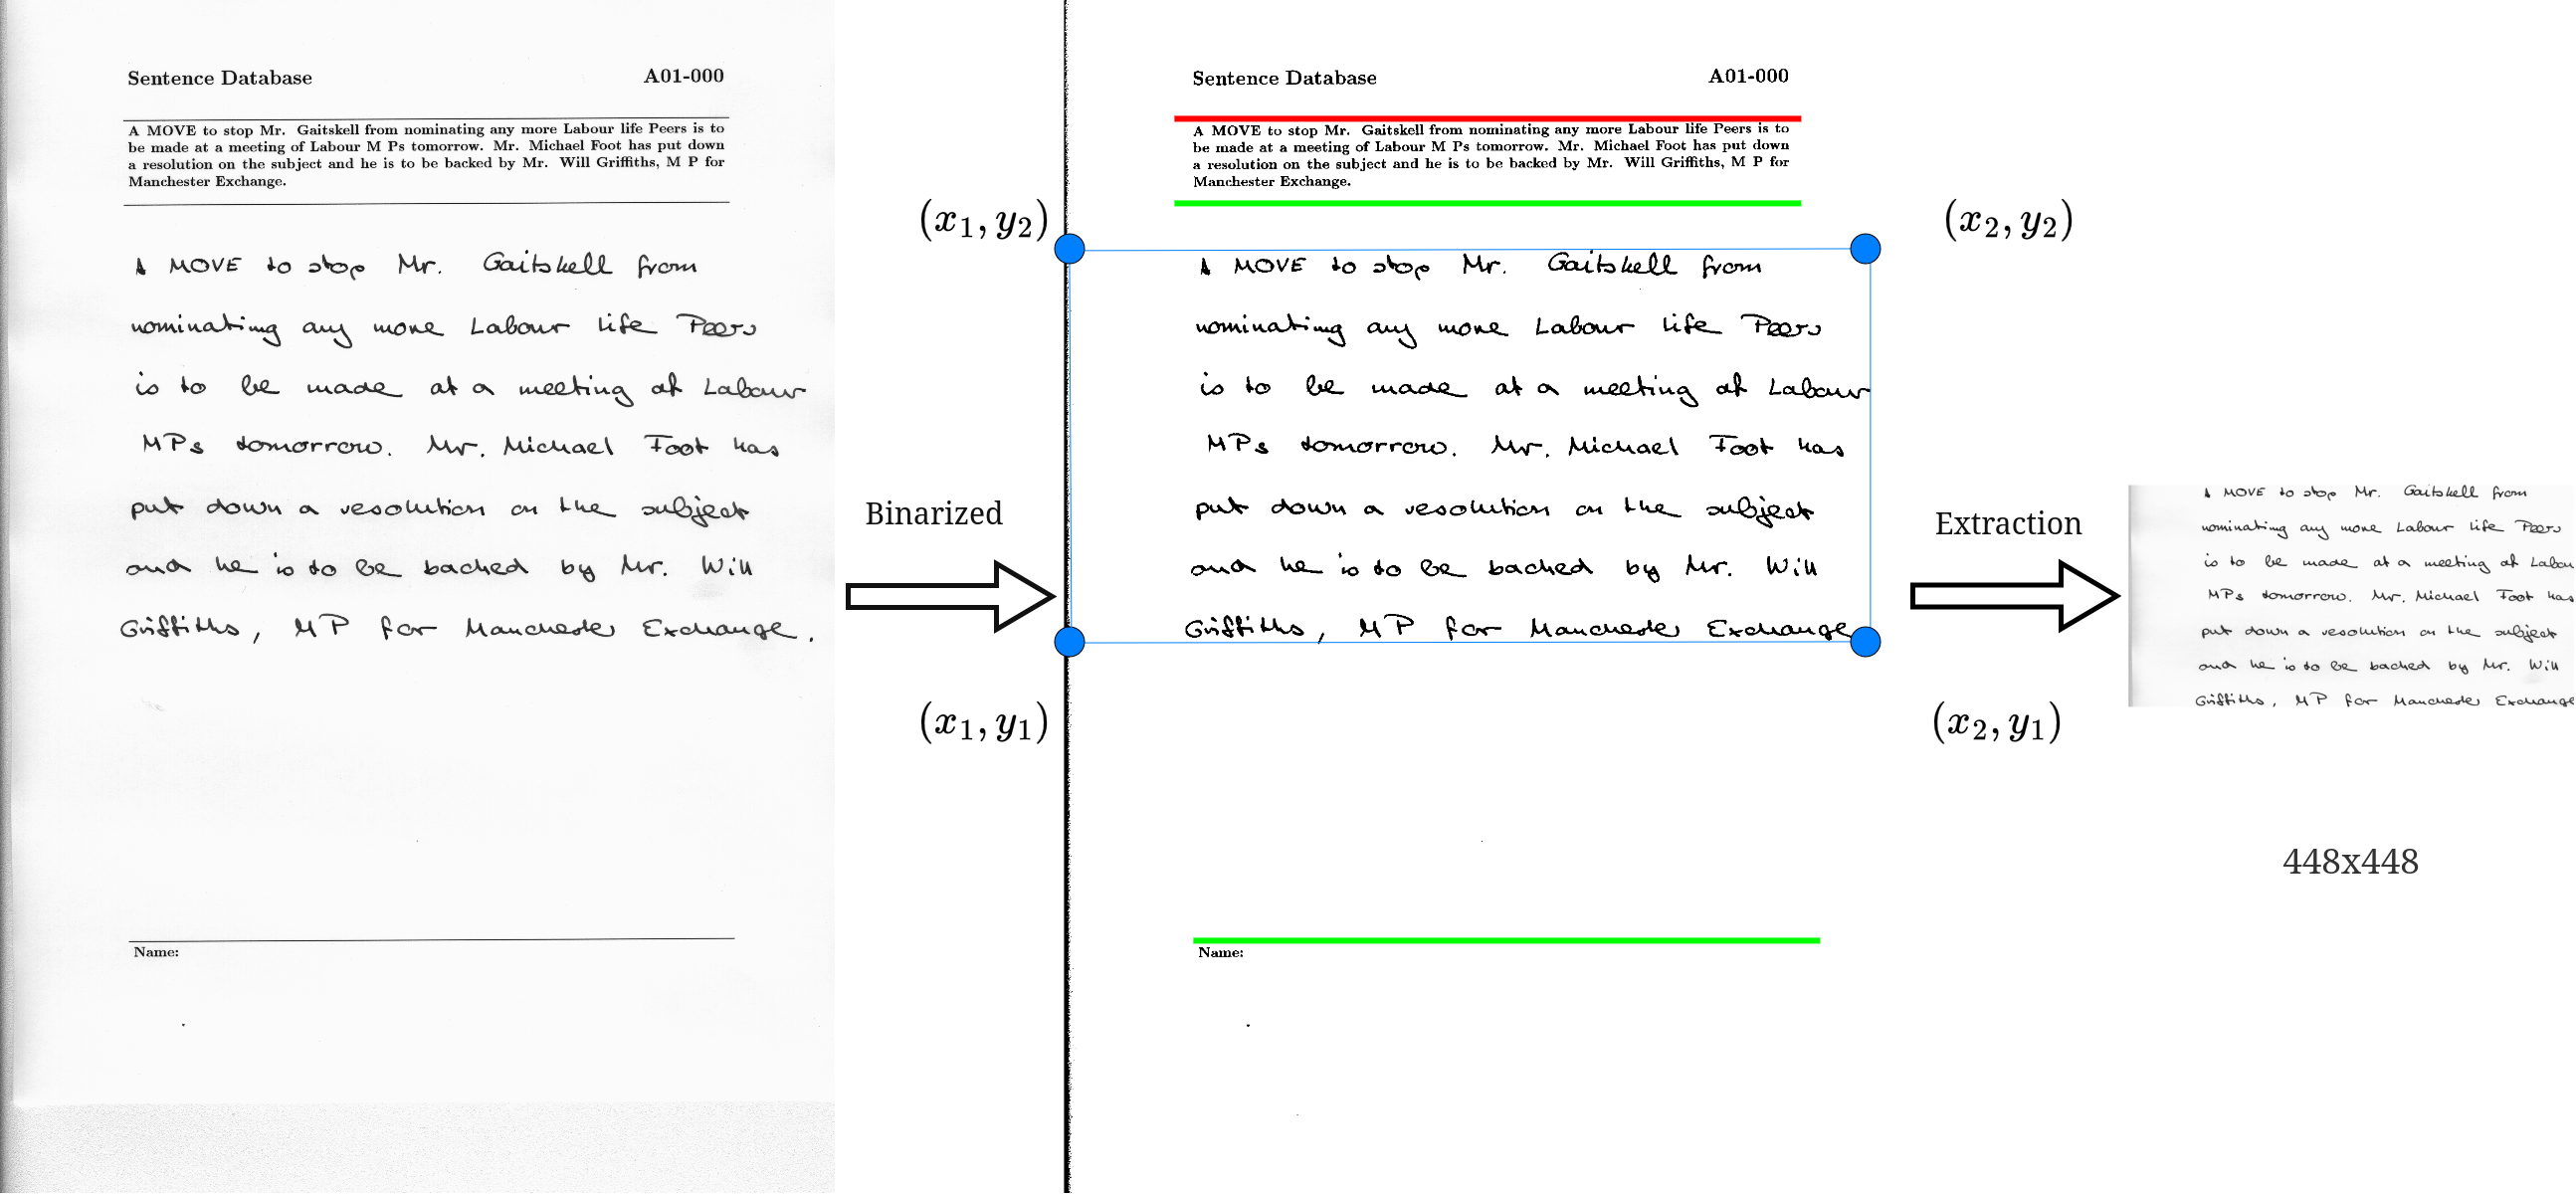
\includegraphics[width=0.9\linewidth]{images/iam-preprocessing.png}
\caption{Preprocessing of an IAM form: the grayscale image (left) is binarized (center) to detect guide lines (red/green, detected by erosion/dilation) and the handwritten text region (blue box); this region is then extracted from the original grayscale image, cropped, and resized to 448×448 pixels (right).}
\label{fig:iam-preprocessing}
\end{figure}

\subsubsection{RIMES Dataset Preprocessing}
\label{app:rimes-preprocessing}

RIMES consists of individual text lines that are processed and stacked vertically to form 448×448 batches. Each line is first converted to grayscale, and an auxiliary Otsu binary mask is derived from it (as described above) purely to guide cropping; only the grayscale line is cropped, resized, and eventually stacked into the output batch. Each line undergoes:

\begin{enumerate}
\item \textbf{Vertical trim:} Removal of rows with $>50\%$ black pixels from top and bottom, computed on the binary mask and applied identically to both the mask and the grayscale line
\item \textbf{Tight cropping:} Bounding-box coordinates computed on the binary mask via the projection-based algorithm ($\rho = 0.018$, Appendix~\ref{app:tight-cropping}), applied to crop the grayscale line
\item \textbf{Height normalization:} For each writer, the minimum observed line height across all their (cropped) lines is computed and clamped to the range $[20, 32]$ pixels, $h_{\min} = \text{clip}(\min_l h_l,\ 20,\ 32)$. All lines from that writer are then resized to height $h_{\min}$, preserving aspect ratio:
\begin{equation}
w' = \lfloor w \cdot h_{\min} / h \rfloor
\end{equation}
If the resulting width $w'$ exceeds the target canvas width (448 px), the line is instead scaled down so that $w' = 448$ and $h' = \lfloor h \cdot 448/w \rfloor \le h_{\min}$. Each resized line is placed on a fixed-size $h_{\min} \times 448$ white canvas, left-aligned and vertically centered with offset $\lfloor (h_{\min} - h')/2 \rfloor$.
\item \textbf{Batching:} Height-normalized lines are vertically stacked into groups of $N_{\text{batch}} = \lfloor 448 / 32 \rfloor - 9 = 5$ lines per batch, producing $448\times448$ canvases per writer. The last batch for a writer is padded with white space if fewer than $N_{\text{batch}}$ lines remain. Figure~\ref{fig:rimes-preprocessing} illustrates this pipeline, from original lines to tight-cropped lines and their grouping into stacked $448\times448$ batches.
\end{enumerate}

Lines exceeding 896 pixels in width (twice the target size) are split at the midpoint before height normalization, to prevent excessive aspect ratio distortion. This produces uniform-height stacked representations suitable for Siamese network training. Note that with $N_{\text{batch}} = 5$ lines of at most 32 px height each, a batch occupies at most 160 of the 448 available vertical pixels; the remaining space is white padding.

\begin{figure}[h]
\centering
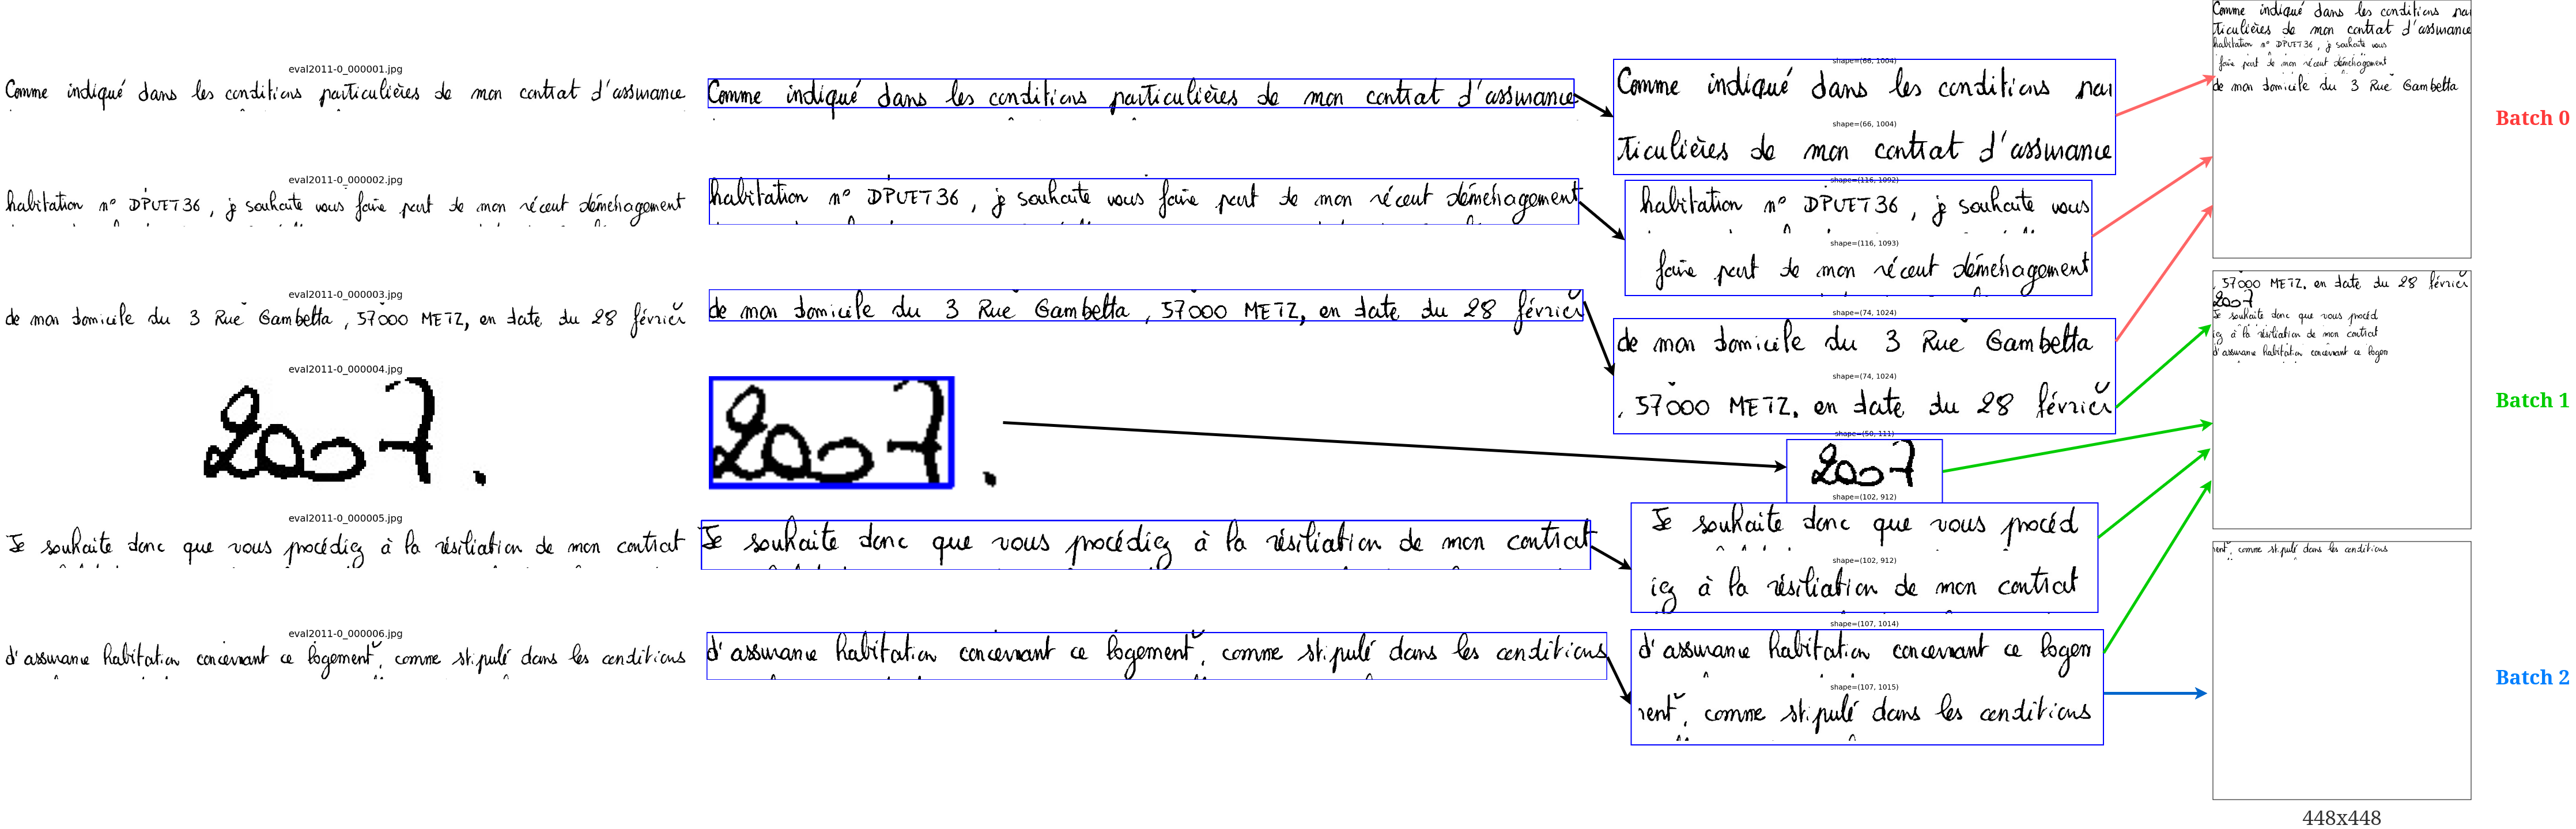
\includegraphics[width=1.0\linewidth]{images/rimes-preprocessing.png}
\caption{Preprocessing of RIMES text lines (for a given author). Each original line (left, e.g. \texttt{eval2011-0\_000001.jpg}) is binarized via Otsu thresholding and tight-cropped (blue bounding boxes, center) using the projection-based algorithm; the corresponding grayscale crop is then extracted (right of center). Cropped lines belonging to the same writer are grouped (colored arrows) and vertically stacked into fixed-size $448\times448$ canvases (right), with unused space padded in white.}
\label{fig:rimes-preprocessing}
\end{figure}

\subsection{Dataset Statistics: Distribution Figures}\label{app:dataset-stats-figures}

Figure~\ref{fig:dataset-distribution} shows the per-author image count distributions for both datasets after preprocessing, complementing the summary statistics of Table~\ref{tab:dataset-stats}. The IAM histogram (top) is dominated by a large spike at 1--2 images per author, with a long, sparse tail extending up to the outlier author with 59 images. The RIMES histogram is comparatively broader and shifted toward higher counts, peaking around 3 batches per author and extending up to 10, reflecting a more even but still right-skewed spread. The boxplot comparison (bottom) further highlights this asymmetry: IAM's interquartile range is narrow and close to zero, with the extreme outlier and long upper whisker revealing a much heavier tail, while RIMES shows a wider, more centrally distributed spread with a shorter relative tail.

\begin{figure}[h]
\centering
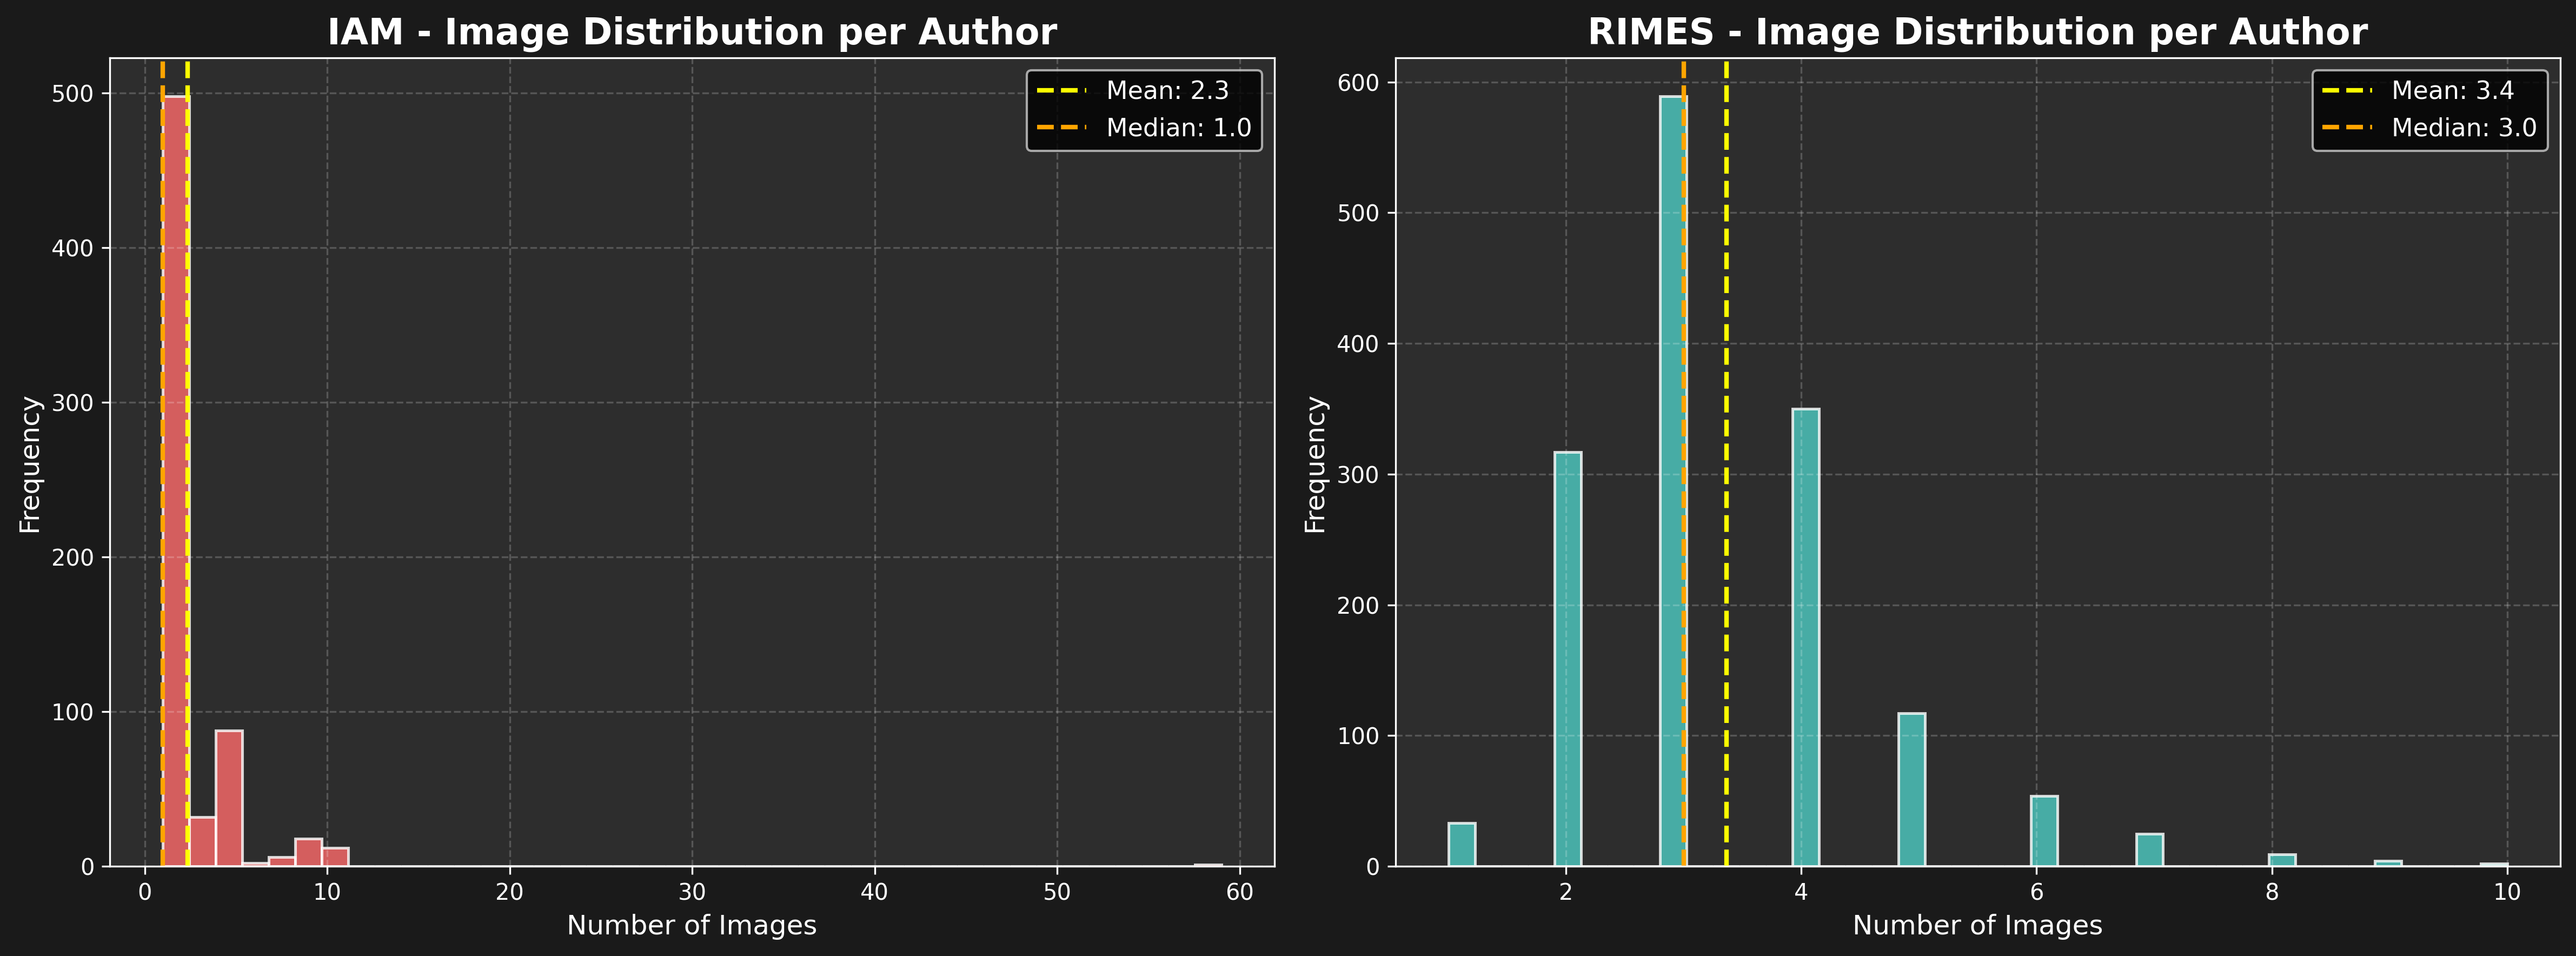
\includegraphics[width=0.65\linewidth]{images/distribution_images.png}
\\[0.5em]
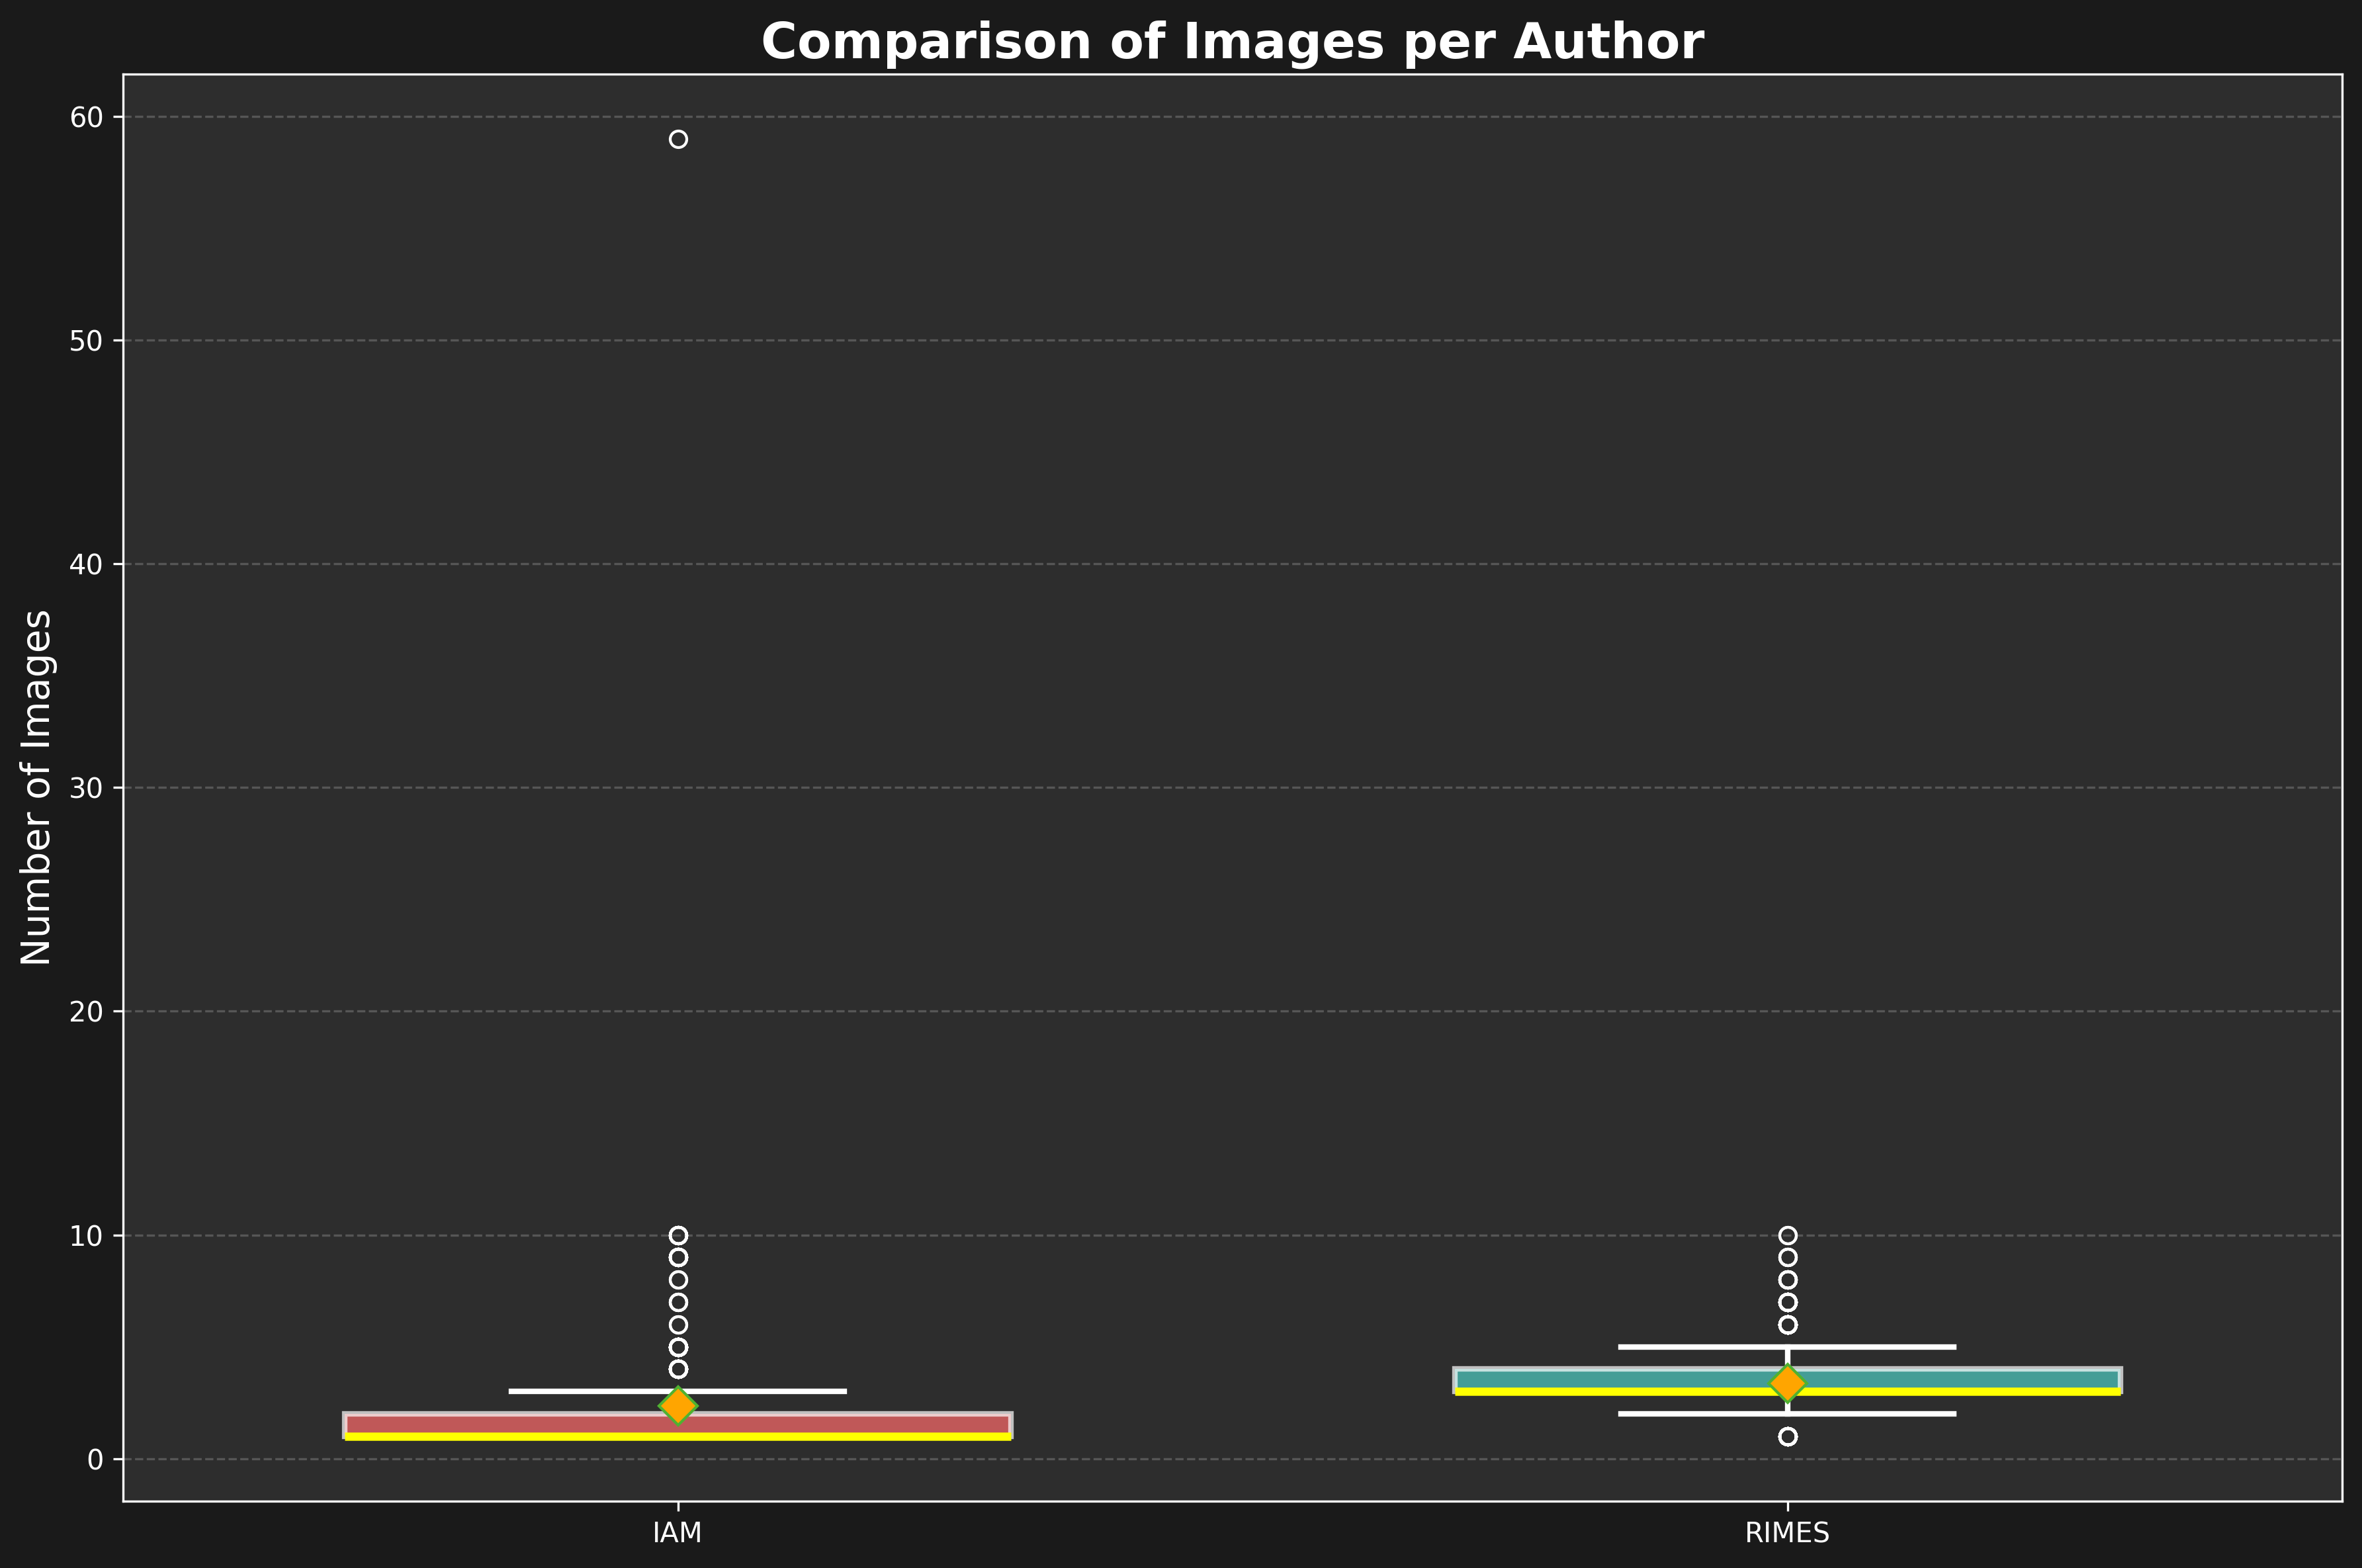
\includegraphics[width=0.7\linewidth]{images/boxplot_comparison.png}
\caption{Distribution of images per author for the preprocessed IAM and RIMES datasets. \textbf{Top:} per-dataset histograms with mean (yellow) and median (orange) overlaid, showing the strong right skew of IAM compared to the broader, more centrally distributed RIMES spread. \textbf{Bottom:} side-by-side boxplot comparison, highlighting the extreme outlier author in IAM (59 images) against the wider but shorter-tailed RIMES distribution (max 10 images).}
\label{fig:dataset-distribution}
\end{figure}

\subsection{Hyperparameter Configuration}\label{app:hyperparams}

Table~\ref{tab:hyperparams-appendix} summarizes the hyperparameter configuration used across the 72-model sweep, 
including values already discussed in the main text (Section~\ref{sec:experiments}) 
and additional training-setup details not otherwise reported, such as maximum epochs, 
embedding dimension, and data-loading workers. Loss-specific margins follow Section~\ref{sec:methodology}: 
$m=1.0$ for Contrastive and $m=0.5$ for Triplet.

\begin{table}[htbp]
\centering
\caption{Hyperparameter configuration shared across the 72 model configurations. Loss-specific settings are indicated where applicable.}
\label{tab:hyperparams-appendix}
\begin{tabular}{ll}
\hline
\textbf{Hyperparameter} & \textbf{Configuration} \\
\hline
Batch size & 16 \\
Maximum epochs & 50 \\
Early stopping & Patience = 5 \\
Image size & $448 \times 448$ pixels \\
Embedding dimension & 32 \\
Margin & 1.0 (Contrastive), 0.5 (Triplet) \\
Positive ratio & 0.5 \\
Dropout & 0.2 \\
Frozen encoder layers & 3 \\
Negative resampling & Every epoch (all losses) \\
Data-loading workers & 4 \\
\hline
\end{tabular}
\end{table}

\subsection{Training Dynamics}\label{app:training-curves}

Figure~\ref{fig:training_curves} reports training and validation loss curves for the ResNet-18 
backbone across all 12 loss$\times$split combinations. Across nearly all configurations, 
training loss decreases monotonically, consistent with stable optimization; however, 
validation-loss behavior differs substantially by loss function and split. Under BCE, 
validation loss tracks training loss relatively closely on the same-dataset splits 
(IAM$\to$IAM, RIMES$\to$RIMES), while the cross-dataset splits show an early divergence between 
the two curves (e.g., IAM$\to$RIMES), consistent with the same-vs-cross-dataset generalization 
gap discussed in Section~\ref{sec:cross-dataset}. Under Contrastive and, more markedly, 
under Triplet Loss, validation loss is considerably noisier and frequently non-monotonic, 
with pronounced oscillations and, in several cases (e.g., Triplet on IAM$\to$IAM and IAM$\to$RIMES), 
no clear downward trend despite steadily decreasing training loss -- indicative of a widening 
train--validation gap rather than smooth joint convergence. Training run lengths also vary 
considerably across configurations, from as few as 6 epochs (Triplet, RIMES$\to$RIMES) to 
over 40 (BCE, IAM$\to$IAM), reflecting the early-stopping criterion (patience 5, Appendix~\ref{app:hyperparams}) 
being triggered at different points depending on the stability of the validation signal for each configuration.

\begin{figure}[htbp]
  \centering
  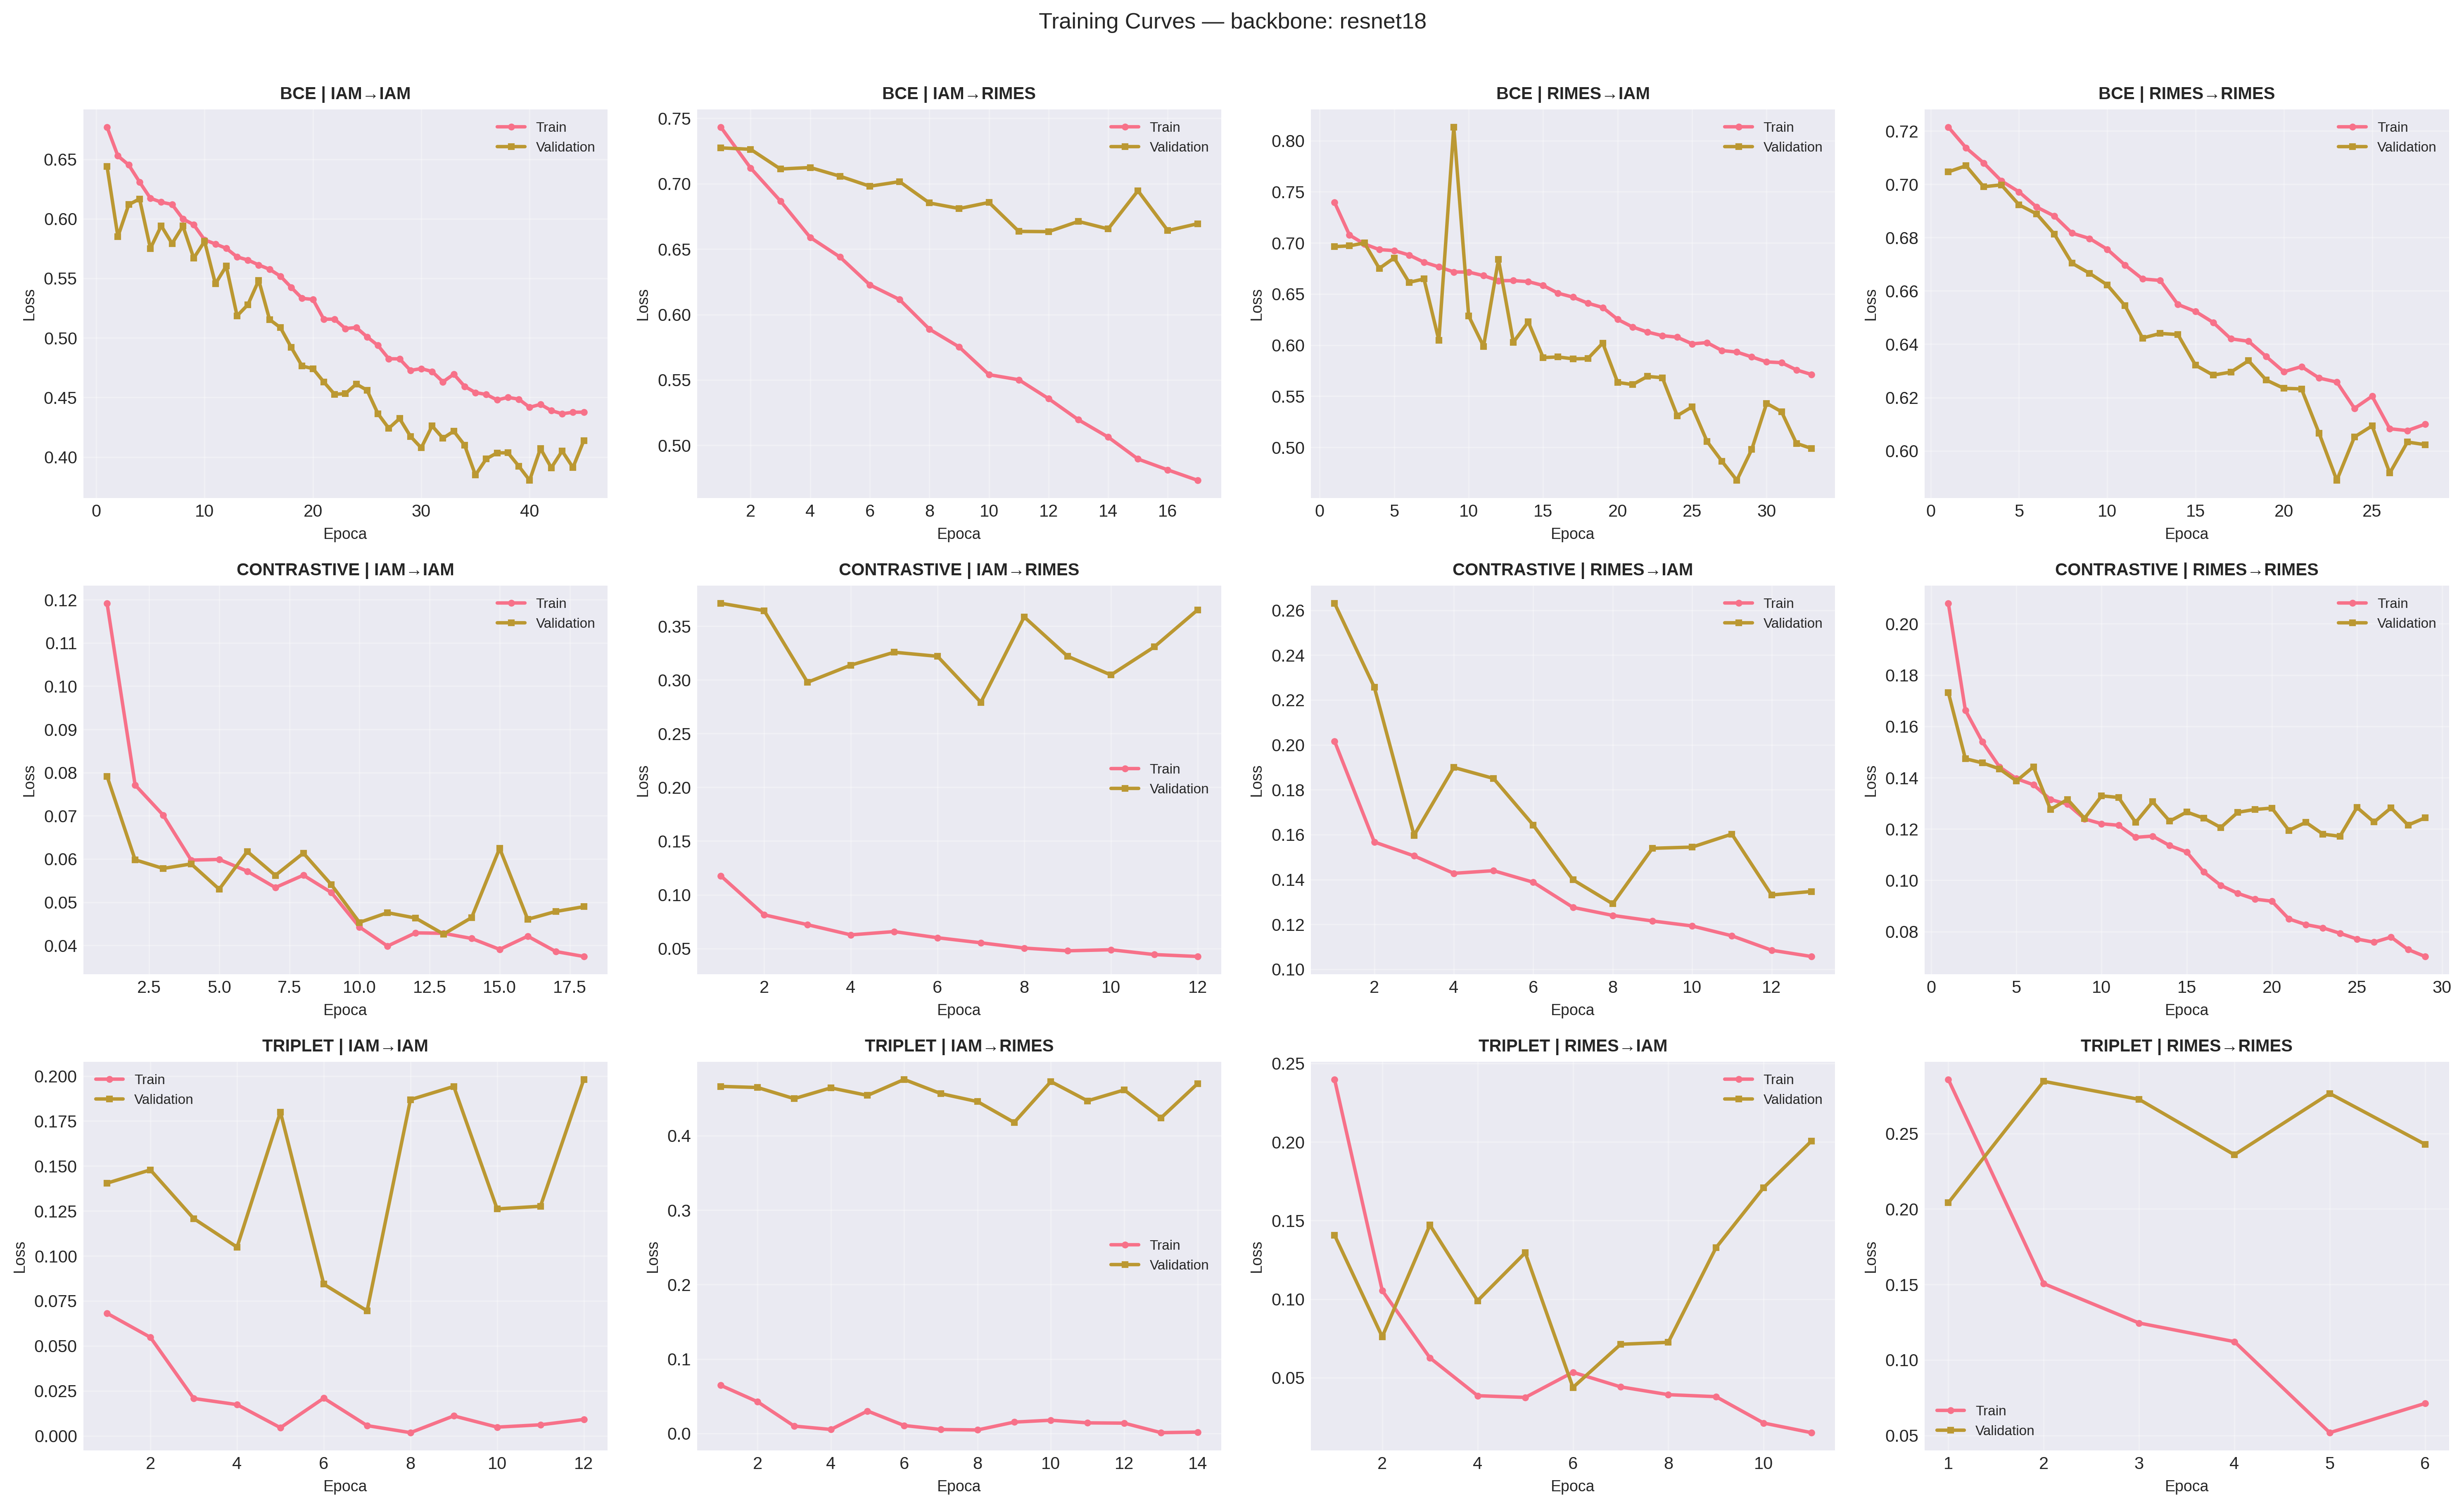
\includegraphics[width=\textwidth]{images/training_history_resnet18.png}
  \caption{Training and validation loss curves, ResNet-18, all 12 loss$\times$split combinations.}
  \label{fig:training_curves}
\end{figure}

\end{appendices}

\newpage

\bibliography{sn-bibliography}

\end{document}